%%%%%%%%%%%%%%%%%%%%%%%%%%%%%%%%%%%%%%%%%%%%%%%%%%%%%%%%%%%%%%%%%%%
%%%%%%%%%%%%%%%%%%%%%%%%%%%%%%%%%%%%%%%%%%%%%%%%%%%%%%%%%%%%%%%%%%%
%           Rapport Contrat SHOM/LA   16CR01                      %
%%%%%%%%%%%%%%%%%%%%%%%%%%%%%%%%%%%%%%%%%%%%%%%%%%%%%%%%%%%%%%%%%%%
%%%%%%%%%%%%%%%%%%%%%%%%%%%%%%%%%%%%%%%%%%%%%%%%%%%%%%%%%%%%%%%%%%%
\documentclass[a4paper,11pt]{report}

\usepackage[utf8]{inputenc}
\usepackage[margin=2.5cm]{geometry}
\usepackage[hidelinks]{hyperref}
\usepackage{titlesec}
\usepackage{lipsum,etoolbox}% http://ctan.org/pkg/{lipsum,etoolbox}
\usepackage[utf8]{inputenc}

\usepackage[french]{babel}
\usepackage[T1]{fontenc}
\frenchbsetup{StandardLists=true} 
\usepackage{enumitem}

%%%%%%%%%%%%%%%%%%%%%%%%%%%%%%%%%%%%%%%%%%%%%%%%%%%%%%%%%%%%%%%%%%%
%%%%%package article 2D Margaux
%%%%%%%%%%%%%%%%%%%%%%%%%%%%%%%%%%%%%%%%%%%%%%%%%%%%%%%%%%%%%%%%%%%
\usepackage{graphicx}
\usepackage{multirow}
\usepackage{tabularx}
\usepackage{color}
\usepackage[fleqn]{amsmath}
\usepackage{amsfonts}
\usepackage{amssymb}
\usepackage{textcomp}
\usepackage{gensymb}
\usepackage{amsxtra}
\usepackage{wasysym}
\usepackage{isomath}
\usepackage{mathtools}
\usepackage{txfonts}
\usepackage{upgreek}
\usepackage{enumerate}
\usepackage{tensor}
\usepackage{pifont}
\usepackage{titlesec}
\usepackage[T1]{fontenc}
\usepackage{fancyhdr}

\usepackage{subcaption}
\usepackage[normalem]{ulem} %25/05
\usepackage{caption}%04/06
\usepackage{afterpage}%04/6
\usepackage{geometry}%05/06
\usepackage{wrapfig}%04/06
\usepackage{chngcntr}
%%%%FIN MH

%%%%%%%%%%%%%%%%%%%%%%%%%%%%%%%%%%%%%%%%%%%%%%%%%%%%%%%%%%%%%%%%%%%
%%%%%%%%  Chapter and Section Numbering (1)               %%%%%%%%%
%%%%%%%%  Francis                                         %%%%%%%%%
%%%%%%%%%%%%%%%%%%%%%%%%%%%%%%%%%%%%%%%%%%%%%%%%%%%%%%%%%%%%%%%%%%%
\usepackage{etoolbox}
\titleformat*{\section}{\large\bfseries}
\titleformat{\chapter}[hang]
    {\normalfont\Large\bfseries}{\chaptertitlename\ \thechapter:}{1em}{\Large}
    \titlespacing*{\chapter} {0pt}{50pt}{40pt}
\usepackage{lipsum}  
\usepackage{pdfpages}

%%%%%%%%%%%%%%%%%%%%%%%%%%%%%%%%%%%%%%%%%%%%%%%%%%%%%%%%%%%%%%%%%%%
%%%%%% Lib doc Lucie%%%%%%%%%%
%%%%%%%%%%%%%%%%%%%%%%%%%%%%%%%%%%%%%%%%%%%%%%%%%%%%%%%%%%%%%%%%%%%
%\usepackage[normalem]{ulem}
\usepackage{array}
%\usepackage{amssymb}
%\usepackage{graphicx}

%\usepackage[backend=biber,
%    style=numeric,
%    sorting=none,
%    isbn=false,
%    doi=false,
%    url=false,
%]{biblatex}\addbibresource{bibliography.bib} %Margaux 

%\usepackage{subfig}
%\usepackage{wrapfig}
%\usepackage{wasysym}
%\usepackage{enumitem}
\usepackage{adjustbox}
\usepackage{ragged2e}
\usepackage[svgnames,table]{xcolor}
%\usepackage{tikz}
\usepackage{longtable}
%\usepackage{changepage}
\usepackage{setspace}
\usepackage{hhline}
\usepackage{multicol}
\usepackage{tabto}
%\usepackage{float}
\usepackage{multirow}
%\usepackage{makecell}
%\usepackage{fancyhdr}
%\usepackage[toc,page]{appendix}
%\usepackage[hidelinks]{hyperref}
%\usetikzlibrary{shapes.symbols,shapes.geometric,shadows,arrows.meta}
%\tikzset{>={Latex[width=1.5mm,length=2mm]}}
%\usepackage{flowchart}\usepackage[paperheight=11.69in,paperwidth=8.27in,left=0.98in,right=0.98in,top=0.98in,bottom=0.98in,headheight=1in]{geometry}
%\usepackage[utf8]{inputenc}
%\usepackage[T1]{fontenc}
\TabPositions{0.5in,1.0in,1.5in,2.0in,2.5in,3.0in,3.5in,4.0in,4.5in,5.0in,5.5in,6.0in,}
\usepackage{chngcntr}
\counterwithin{figure}{section}
\counterwithin{table}{section}

%\urlstyle{same}
%%%%%% Lib doc Lucie%%%%%%%%%%

%%%%%%%%%%%%%%%%%%%%%%%%%%%%%%%%%%%%%%%%%%%%%%%%%%%%%%%%%%%%%%%%%%%
% Title Page
%%%%%%%%%%%%%%%%%%%%%%%%%%%%%%%%%%%%%%%%%%%%%%%%%%%%%%%%%%%%%%%%%%%
\title{
Modélisation des fines échelles internes\\ dans la région du détroit de Gibraltar.\\
\bigskip\bigskip
\large{Contrat SHOM / UPS 16CR01.}\\
\bigskip\bigskip\bigskip\bigskip\bigskip\bigskip
Groupe Croco, Laboratoire d'Aérologie}

\author{Lucie Bordois\footnote{Post-Doctorante.}, Margaux Hilt\footnote{Stagiaire M2 puis doctorante SDUEE 
Toulouse.},
Eric Chassignet\footnote{Professeur invité.},
Laurent Roblou, Cyril Nguyen, Francis Auclair\footnote{Permanents CNRS et UPS au Laboratoire d'Aérologie.}
}
%%%%%%%%%%%%%%%%%%%%%%%%%%%%%%%%%%%%%%%%%%%%%%%%%%%%%%%%%%%%%%%%%%%
% Bibliographie (Margaux)
%%%%%%%%%%%%%%%%%%%%%%%%%%%%%%%%%%%%%%%%%%%%%%%%%%%%%%%%%%%%%%%%%%%
\makeatletter %remove numbers in bibliography
\renewcommand\@biblabel[1]{}
\makeatother
%%%%%%%%%%%%%%%%%%%%%%%%%%%%%%%%%%%%%%%%%%%%%%%%%%%%%%%%%%%%%%%%%%%
%%%%%%%%%%%%%%%%%%%%%%%%%%%%%%%%%%%%%%%%%%%%%%%%%%%%%%%%%%%%%%%%%%%
%                   Début du document                             %
%%%%%%%%%%%%%%%%%%%%%%%%%%%%%%%%%%%%%%%%%%%%%%%%%%%%%%%%%%%%%%%%%%%
%%%%%%%%%%%%%%%%%%%%%%%%%%%%%%%%%%%%%%%%%%%%%%%%%%%%%%%%%%%%%%%%%%%
\begin{document} 

%%%%%%%%%%%%%%%%%%%%%%%%%%%%%%%%%%%%%%%%%%%%%%%%%%%%%%%%%%%%%%%%%%%
%%%%%%%%  Chapter and Section Numbering (2)               %%%%%%%%%
%%%%%%%%  Francis                                         %%%%%%%%%
%%%%%%%%%%%%%%%%%%%%%%%%%%%%%%%%%%%%%%%%%%%%%%%%%%%%%%%%%%%%%%%%%%%
\renewcommand{\thepage}{}
\renewcommand{\thechapter}{\Roman{chapter}}
\renewcommand{\thesection}{\arabic{section}}
\setcounter{secnumdepth}{4}
\newcommand*{\newpar}{%
  \ifsubsection\else\stepcounter{subsection}\fi
  \paragraph{}}
\setcounter{figure}{0}
\renewcommand{\thefigure}{\Roman{chapter}.\arabic{section}.\arabic{figure}}
\setcounter{table}{0}
\renewcommand{\thetable}{\Roman{chapter}.\arabic{section}.\arabic{table}}
%%% A conditional for knowing whether a \subsection
%%% command has been issued

\author{Lucie Bordois\footnote{Post-Doctorante.}, Margaux Hilt\footnote{Stagiaire M2 puis doctorante SDUEE Toulouse.},
Eric Chassignet\footnote{Professeur invité.},
Laurent Roblou, Cyril Nguyen, Francis Auclair\footnote{Permanents CNRS et UPS au Laboratoire d'Aérologie.}
}

%%%%%%%%%%%%%%%%%%%%%%%%%%%%%%%%%%%%%%%%%%%%%%%%%%%%%%%%%%%%%%%%%%%
% Bibliographie (Margaux)
%%%%%%%%%%%%%%%%%%%%%%%%%%%%%%%%%%%%%%%%%%%%%%%%%%%%%%%%%%%%%%%%%%%
\makeatletter %remove numbers in bibliography
\renewcommand\@biblabel[1]{}
\makeatother
%%%%%%%%%%%%%%%%%%%%%%%%%%%%%%%%%%%%%%%%%%%%%%%%%%%%%%%%%%%%%%%%%%%
%%%%%%%%%%%%%%%%%%%%%%%%%%%%%%%%%%%%%%%%%%%%%%%%%%%%%%%%%%%%%%%%%%%
%                   Début du document                             %
%%%%%%%%%%%%%%%%%%%%%%%%%%%%%%%%%%%%%%%%%%%%%%%%%%%%%%%%%%%%%%%%%%%
%%%%%%%%%%%%%%%%%%%%%%%%%%%%%%%%%%%%%%%%%%%%%%%%%%%%%%%%%%%%%%%%%%%

%%%%%%%%%%%%%%%%%%%%%%%%%%%%%%%%%%%%%%%%%%%%%%%%%%%%%%%%%%%%%%%%%%%
%%%%%%%%  Chapter and Section Numbering (2)               %%%%%%%%%
%%%%%%%%  Francis                                         %%%%%%%%%
%%%%%%%%%%%%%%%%%%%%%%%%%%%%%%%%%%%%%%%%%%%%%%%%%%%%%%%%%%%%%%%%%%%
\renewcommand{\thepage}{}
\renewcommand{\thechapter}{\Roman{chapter}}
\renewcommand{\thesection}{\arabic{section}}
\setcounter{secnumdepth}{4}
\newcommand*{\newpar}{%
  \ifsubsection\else\stepcounter{subsection}\fi
  \paragraph{}}
\setcounter{figure}{0}
\renewcommand{\thefigure}{\Roman{chapter}.\arabic{section}.\arabic{figure}}
\setcounter{table}{0}
\renewcommand{\thetable}{\Roman{chapter}.\arabic{section}.\arabic{table}}

%%% A conditional for knowing whether a \subsection
%%% command has been issued
\newif\ifsubsection

%%% Set the conditional to true after \subsection
%%% and reset the paragraph counter
\preto{\subsection}{\global\subsectiontrue\setcounter{paragraph}{0}}
%%% Reset it to false after \section
\preto{\section}{\global\subsectionfalse}

\counterwithin*{paragraph}{section}
\makeatletter
\renewcommand\paragraph{%
    \@startsection{paragraph}{4}{0mm}%
       {-\baselineskip}%
       {.5\baselineskip}%
       {\normalfont\normalsize\bfseries}}
\makeatother
\renewcommand{\theparagraph}{\alph{paragraph}.}

\maketitle
\newpage
	 \null
\newpage
 
{\setlength{\baselineskip}{0.8\baselineskip}
\tableofcontents\par}
\renewcommand{\thepage}{\arabic{page}}
\setcounter{page}{1}
%\tableofcontents

\maketitle
\newpage
	 \null
\newpage

\selectlanguage{french}
%%%%%%%%%%%%%%%%%%%%%%%%%%%%%%%%%%%%%%%%%%%%%%%%%%%%%%%%%%%%%%%%%%%
%%%%%%%%%%%%%%%%%%%%%%%%%%%%%%%%%%%%%%%%%%%%%%%%%%%%%%%%%%%%%%%%%%%
%%% Chapitre Introduction
%%%%%%%%%%%%%%%%%%%%%%%%%%%%%%%%%%%%%%%%%%%%%%%%%%%%%%%%%%%%%%%%%%%
%%%%%%%%%%%%%%%%%%%%%%%%%%%%%%%%%%%%%%%%%%%%%%%%%%%%%%%%%%%%%%%%%%%
\chapter{Introduction}
\label{chapitreintroduction}

\section{Contexte, généralités}
 \noindent\textbf{\textit{Extrait du Cahier des clauses techniques particulières du contrat de recherche Gibraltar 16CR01}}\\
Cette étude s'inscrit dans le cadre du projet stratégique PROTEVS (\textit{prévision océanique, turbidité, écoulement, vagues et sédimentologie}) qui vise l’amélioration des systèmes d’analyse et de prévision décrivant l’environnement marin en temps réel. Il s’agit de prendre en compte les couplages entre l’état de mer (vagues) et la circulation océanique (courants à plus grande échelle), et de réaliser des études et recherches pour la représentation des petites échelles, des paramètres biochimiques et de la dynamique sédimentaire. PROTEVS est un programme d’études amont (PEA 082401) financé par la DGA.\\

\noindent Dans ce contexte, les objectifs du contrat de recherche \textit{Gibraltar 16CR01} entre le SHOM et le laboratoire d'Aérologie  sont : 

\begin{itemize}[label=\textbullet]
 \item d’améliorer la connaissance des processus océaniques et côtiers impactant les opérations militaires (action continue de ``recherche amont``).
 \item d'étudier la faisabilité de systèmes permettant la reconstitution en temps réel (analyse) de l’environnement hydrodynamique (état de mer, courants, température, salinité) ainsi que de son évolution possible (prévision).
d’étudier des possibilités d’y intégrer des paramètres biogéochimiques (matière en suspension, mobilité des sols, transparence, visibilité).
\end{itemize}

\noindent  Le projet concerne l'amélioration d’un modèle numérique décrivant la circulation à petite échelle de l’océan. Il comporte trois tâches distinctes\footnote{La Tâche 3 a fait l'objet d'un avenant au contrat initial signé en 2016.}:
\begin{itemize}[label=\textbullet]
\item la première tâche consiste à implémenter un modèle numérique qui puisse totalement relaxer l’hypothèse d’hydrostaticité dans la région du détroit de Gibraltar et à procéder à une évaluation (coût calcul/performance) de la maquette numérique ainsi proposée.
\item la deuxième tâche concerne la généralisation du système de coordonnées verticales, à partir d’une approche ALE (\textit{Arbitrary Lagrangian-Eulerian coordinate}).
\item la troisième tâche concerne enfin la fourniture d'un produit numérique élaboré sur la base des maquettes numériques du détroit de Gibraltar telles que mises en place à la tâche 1.
\end{itemize}

\label{simuFE}
\section{Simulation des "fines échelles" \textit{(Groupe de recherche CROCO-Aérologie) }}

\noindent \textit{\textbf{Dynamique des fines échelles}}\\
Le groupe de modélisation océanique du Laboratoire d'Aérologie\footnote{Laboratoire de l'Observatoire Midi-Pyrénées}, contractant du projet Gibraltar 16CR01 et devenu en 2018 ''groupe CROCO-Aérologie``, étudie la \textit{dynamique des fines échelles océaniques} depuis maintenant une dizaine d'années. La qualification de \textit{fines échelles} englobe ici de façon très large une gamme de processus présentant une \textit{extension horizontale plus fine que le premier rayon de Rossby}. Cette définition couvre par conséquent des mécanismes et des processus dynamiques très hétérogènes:
\begin{itemize}
 \item les ondes de gravité (ondes de surface ou ondes internes) ou encore les ondes acoustiques ainsi que les mécanismes de génération et de déferlement associés à ces différents types d'ondes,
 \item les instabilités primaires de Kelvin-Helmholtz, les instabilités convectives... ainsi que la cascade turbulente directe initiée par ces instabilités primaires et conduisant au mélange diapycnal,
 \item les processus localisés liés au contrôle hydraulique des masses d'eau (ressauts hydrauliques...)
\end{itemize}
En parallèle, un projet pédagogique (SiGeoS) dédié à la turbulence géophysique a été mis en place aux niveaux Licence et Master par le groupe CROCO-Aérologie\footnote{SigeoS est un projet IDEX-Toulouse \textit{Pédagogie Innovante} proposant enseignement théorique et enseignement pratique en laboratoire et numérique. Le volet en Laboratoire du projet pédagogique SiGeoS est une collaboration avec le CNRM (Météo-France/CNRS)}. \\

\noindent \textit{\textbf{Simulation des grandes échelles turbulentes (LES)}}\\
Pour mener à bien ce projet de recherche et son alter-ego pédagogique, le groupe CROCO-Aérologie a été amené à faire évoluer ses outils numériques et en particulier son code numérique d'océan. La simulation des ''fines échelles océaniques`` nécessite en effet la mise en place d'une ''simulation des grandes structures turbulentes`` (en anglais \textit{LES}, pour Large Eddy Simulation). Les codes océaniques à toit libre (explicite) et pas-de-temps séparés (\textit{time-splitting} en anglais) devenus des classiques en modélisation océanique côtière et régionale au milieu des années 90 s'appuient tous sur l'hypothèse hydrostatique et ne permettent donc pas la simulation numérique tri-dimensionnelle des structures en vorticité comme le requière la LES. Le groupe CROCO-Aérologie a donc développé un code à toit libre et pas-de-temps séparés s'appuyant de façon originale sur un coeur non-hydrostatique (NH). Un algorithme par correction de pression (\textit{SNH}) a tout d'abord été implémenté dans le code Symphonie (Auclair et al., 2011). L'association de cet algorithme NH avec un schéma temporel à pas-de-temps séparés se révélant inappropriée\footnote{Association correction de pression / schéma temporel à pas-de-temps séparés: pour être efficace la correction de pression doit être implémentée dans le mode interne (lent), l'intégration et la correction du mode externe est numériquement mal posé et entraîne la génération de modes numériques potentiellement instables. D'un point de vue physique, les ondes de surface NH (ondes courtes) présentent en effet un cisaillement vertical de vitesse résolu par le seul mode lent (3D): le rapport des pas-de-temps des deux modes doit donc être proche de 1...}, un algorithme original, cette fois compressible (dit \textit{''non Boussinesq``}) a alors été proposé et implémenté en mode recherche dans le même code Symphonie (\textit{SNBQ}) (Auclair et al., 2018). \\

\noindent \textit{\textbf{Non-hydrostaticité et performances numériques}}\\
Ces développements algorithmiques laissant entrevoir des perspectives prometteuses pour l'étude des processus dynamiques, la nécessité de réaliser d'importants gains de performances a alors conduit à une remise en cause globale des schémas temporels, des schémas d'advection d'ordre réduit et des schémas de turbulence anisotropes généralement utilisés en océanographie régionale et côtière et plus spécifiquement dans \textit{SNBQ}. L'algorithme non-hydrostatique, non-Boussinesq développé en mode recherche dans \textit{SNBQ} a donc été implémenté dans ROMS-AGRIF rebaptisé CROCO (Auclair et al., \textit{publication en cours}). \\
Des gains de performances importants (à minima un ordre de grandeur) ont ainsi pu être réalisés grâce tout d'abord à plusieurs spécificités du code ROMS (Shchepetkin et McWilliams, 2005): 
\begin{itemize}
	\item son écriture et sa structure épurée facilitant la gestion de la \textit{mémoire-cache} des processeurs, 
	\item ou encore son implantation MPI particulièrement efficace. 
\end{itemize}

\noindent Une réécriture et une restructuration complète de l'algorithme non-hydrostatique, non-Boussinesq en un coeur numérique bi-modal\footnote{\textit{SNBQ} présente un coeur numérique à trois modes (modes interne(3D)/externe(2D)/NBQ(3D) alors que CROCO-NBQ est bi-modal (modes lent et rapide (NBQ) tous deux 3D.} ont finalement permis d'atteindre un niveau de performance numérique compatible avec la simulation \textit{LES} de la région du détroit de Gibraltar.\\
Le développement, les gains de performances et la consolidation du cœur numérique CROCO-NBQ ont pu être menés à bien grâce aux compétences complémentaires des instituts et universités associés au GdR CROCO (\textit{SHOM, IFREMER, INRIA, IRD}, \textit{INSU-CNRS} et \textit{Université de Toulouse Paul Sabatier}). Le code CROCO, base de la présente étude, est un véritable outil \textit{communautaire} de part son développement, son utilisation et sa distribution.\\


\section{Le détroit de Gibraltar: un "démonstrateur"}

En plus de ses enjeux stratégiques, le détroit de Gibraltar présente un indéniable intérêt en termes de dynamique océanique. A l'échelle de la circulation générale, il est l'unique lieu d'échange entre les bassins méditerranéen et Nord-Atlantique. La bathymétrie peu profonde du détroit impose un contrôle hydraulique sur ces échanges entraînant ressauts hydrauliques, générations d'ondes internes de grande amplitude, instabilités en cascade... autant de mécanismes qui induisent in fine un mélange intense des deux masses d'eau.\\
La qualité des prévisions de la circulation générale et des principales masses d'eau en Atlantique Nord et en Méditerranée dépend donc pour partie de notre capacité à comprendre et à simuler les principaux mécanismes et processus dynamiques de \textit{fine échelle} à l'œuvre dans le détroit de Gibraltar.\\

\noindent \textbf{\textit{Expertise dynamique}}\\
Lors du lancement du projet Gibraltar 16CR01 en 2016, le groupe CROCO-Aérologie avait déjà consacré une première étude à la région du détroit de Gibraltar avec la thèse de Lucie Bordois (Bordois, 2015, Bordois et al. 2016, Bordois et al., 2017). Cette étude avait permis :
\begin{itemize}
	\item  d'évaluer la "faisabilité" d'une simulation numérique des \textit{fines échelles} dans le détroit. Une maquette reposant sur une section verticale 2D avec les codes de recherche SNH puis SNBQ a ainsi été développée, les coûts de calcul et la qualité de la dynamique simulée ont été évalués.
	\item de réaliser une analyse approfondie des régimes dynamiques induits par la présence d'un détroit.
	\item de mettre en évidence la génération d'ondes internes de grande amplitude de Mode 1 et 2 au dessus des seuils de Camarinal et d'Espartel.
\end{itemize}
La thèse de Lucie Bordois a aussi confirmé la nécessité de franchir un cap en matière d'efficacité numérique: le code de recherche SNBQ se devait d'évoluer vers des méthodologies "massivement parallèles" efficaces. Une approche communautaire apparaissait alors clairement comme la seule alternative pouvant rapidement ouvrir les portes de la LES en océanographie. \\

\noindent \textbf{\textit{L'efficacité numérique: un enjeu communautaire}}\\
La région du détroit a par conséquent été choisie par le GdR CROCO comme "zone test" \textit{(démonstrateur}) et le groupe CROCO-Aérologie a concentré sur cette région l'essentiel de ses efforts de développements du cœur numérique non-hydrostatique et non-Boussinesq \textit{CROCO-NBQ} avec plusieurs objectifs:
\begin{itemize}
 \item \textit{mieux comprendre et mieux décrire la dynamique de fine échelle dans la région du détroit}. Les mécanismes de génération des ressauts hydrauliques, des ondes stationnaires orographiques \footnote{\textit{"Ocean lee waves"} en anglais.}, des ondes internes de grande amplitude (ondes solitaires) et des instabilités primaires     constituent autant de clés pour aborder la difficile problématique du mélange des masses d'eau (dans cette région et plus généralement dans l'océan global).
 \item  \textit{mettre en place par étape une maquette LES du détroit}. Cette maquette doit permettre à minima la simulation explicite des instabilités primaires se développant à l'interface des eaux méditerranéennes et atlantiques et doit in fine offrir une représentation réaliste et précise du mélange diapycnal intense entre ces deux masses d'eaux.
 \item \textit{comprendre et simuler la formation du jet méditerranéen dans le détroit}. C'est dans la région du détroit que cette composante importante de la circulation dans le bassin Nord-Atlantique prend naissance et acquière ses principales caractéristiques (densité, vorticité potentielle...).
\end{itemize}

\section{Méthodologie et engagements contractuels}

\noindent\textit{\textbf{Une hiérarchie de maquettes}}\\
Le groupe CROCO-Aérologie a choisi une méthodologie de développement numérique et d'exploration de la dynamique s'appuyant sur une hiérarchie de \textit{maquettes numériques} de complexité et de réalisme croissants:
\begin{itemize}
\item raffinement par étape de la physique à partir de maquettes hydrostatiques puis non-hydrostatiques et non-Boussinesq,
\item raffinement d'échelles avec des résolutions spatiales de l'ordre de quelques centaines de mètres (220 m pour la maquette NH-REF) réduites dans un second temps à seulement quelques dizaines de mètres (45 m pour la maquette NH-HR).
\end{itemize}
Il est à noter que la résolution la plus basse proposée dans le cadre du présent rapport est déjà 5 fois plus fine que la résolution initialement proposée dans le cadre du contrat de recherche Gibraltar 16CR1. En effet, la "\textit{résolution dans une gamme équivalente à celles de la maquette HYCOM utilisée par le SHOM pour cette région}" (soit environ 1.8 km) proposée dans le contrat s'est révélée beaucoup trop grande pour explorer les \textit{fines échelles} dans la région du détroit. Les résolutions de l'ordre de 220 m (maquette NH-REF) et de 45 m (maquette NH-HR) permettent de représenter et d'explorer les ondes internes de grande amplitude \textit{(ondes solitaires)} et les instabilités dynamiques primaires se développant entre les deux masses d'eau et conduisant à l'intensification locale du mélange (pour la résolution la plus fine seulement). Le travail en amont sur les performances numériques du coeur CROCO-NBQ (Section \ref{simuFE}) a permis de réaliser ce saut en résolution.\\
\noinden Chaque nouvelle maquette a été implémentée et sa dynamique explorée en deux temps. Des sections verticales bi-dimensionnelles alignées avec le transect principal de la campagne Gibraltar Experiment (Farmer et Armi, 1988) ont tout d'abord été mises en place, leur dynamique étant dans la foulée détaillée. Cette stratégie de dégradation des maquettes 3D est un choix reposant sur deux objectifs principaux:
\begin{itemize}
\item réduire les coûts de calcul inhérents à la mise au point des nouveaux algorithmes et des nouveaux schémas numériques,
\item simplifier la dynamique océanique complexe en l'assimilant à celle d'un canal hypothétiquement aligné avec l'axe du détroit.
\end{itemize}

\noindent\textit{\textbf{Une dynamique simplifiée}}\\
Un choix méthodologique fort a ensuite consisté, pour chaque maquette, à ne retenir que les forçages et les caractéristiques hydrologiques indispensables à la mise en place de la dynamique à explorer:
\begin{itemize}
\item Identifiée comme un élément clé de la dynamique régionale, une bathymétrie précise de la région du détroit a été fournie par le SHOM.
\item Les ondes et les courants de marée sont imposés de façon réaliste aux frontières des différentes maquettes.
\item Les deux principales masses d'eau (d'origine atlantique et méditerranéenne) ont dans un premier temps été simulées via une stratégie dite en \textit{Lock-Exchange} avant d'être forcées directement à partir des prévisions du modèle de circulation à "haute résolution" MIT-GCM fournies par l'ENEA \footnote{http://www.enea.it/it/seguici/pubblicazioni/pdf-volumi/cresco-report-2016.pdf. Nous remercions G. Sannino et l'ENEA pour ces sorties de simulation ainsi que pour l'accueil à Rome (Italie) de Lucie Bordois, alors post-doctorante dans le cadre du présent contrat.}.
\item Les forçages atmosphériques et telluriques ont, en première approximation, été négligés.
\end{itemize}

%%%%%%%%%%%%%%%%%%%%%%%%%%%%%%%%%%%%%%%%%%%%%%%%%%%%%%%%%%%%%%%%%%%
%%%%%%%%%%%%%%%%%%%%%%%%%%%%%%%%%%%%%%%%%%%%%%%%%%%%%%%%%%%%%%%%%%%
% Chapitre: Modélisation des fines échelles
%%%%%%%%%%%%%%%%%%%%%%%%%%%%%%%%%%%%%%%%%%%%%%%%%%%%%%%%%%%%%%%%%%%
%%%%%%%%%%%%%%%%%%%%%%%%%%%%%%%%%%%%%%%%%%%%%%%%%%%%%%%%%%%%%%%%%%%
\chapter{Modélisation des fines échelles dans le détroit de Gibraltar\\}
\label{chapitremodele}

La Tâche 1 du contrat Gibraltar 16CR01 est scindée en deux sous-tâches portant respectivement sur:
\begin{itemize}
\item{le développement et la validation d’une hiérarchie de maquettes hydrostatiques et non-hydrostatiques de la région du détroit de Gibraltar \textit{(Tâche 1.1)}}
\item{la dynamique à haute résolution dans le détroit de Gibraltar \textit{(Tâche 1.2)}}
\end{itemize}

\noindent Les maquettes et la dynamique qu'elles ont respectivement permis d'explorer sont maintenant décrites par ordre croissant de complexité pour offrir un rendu graduel des résultats obtenus. L'ordre proposé correspond de plus à la chronologie de développement et d'exploration choisie. \\

La Tâche 2 a été confiée à Eric Chassignet, visiteur scientifique au laboratoire d'Aérologie dans le cadre du présent contrat. Elle a pour objectif d'évaluer la pertinence d'une évolution du système de coordonnées verticales du code communautaire CROCO.

%%%%%%%%%%%%%%%%%%%%%%%%%%%%%%%%%%%%%%%%%%%%%%%%%%%%%%%%%%%%%%%%%%%
%%%%%%%%%%%%%%%%%%%%%%%%%%%%%%%%%%%%%%%%%%%%%%%%%%%%%%%%%%%%%%%%%%%
%%% Sections verticales 2D
%%%%%%%%%%%%%%%%%%%%%%%%%%%%%%%%%%%%%%%%%%%%%%%%%%%%%%%%%%%%%%%%%%%
%%%%%%%%%%%%%%%%%%%%%%%%%%%%%%%%%%%%%%%%%%%%%%%%%%%%%%%%%%%%%%%%%%%
\section{Sections verticales 2D: maquettes NH-REF et NH-HR \textit{(Tâche 1.1)}}
\label{section2D}

\noindent\fbox{\noindent\begin{minipage}{1\textwidth}
Une configuration numérique simple 2D est implémentée dans le détroit de Gibraltar avec le code communautaire CROCO dans sa version non-hydrostatique, non-Boussinesq (CROCO-NBQ). Cette configuration est peu coûteuse en temps de calcul et incorpore la bathymétrie le long de l'axe du détroit avec sa configuration de seuils (Farmer et Armi, 1988, programme \textit{Gibraltar Experiment}). Dans l'élaboration de cette configuration, une attention toute particulière a été apportée au rôle de la pseudo-force de Coriolis sur l'échange moyen simulé lors de l'initialisation par \textit{lock-exchange}.\\
Malgré les défauts inhérents à une représentation 2D-verticale (nécessairement limitée dynamiquement et non représentative des effets longitudinaux comme le contrôle dans le détroit de Tarifa), la configuration proposée permet de représenter de façon réaliste les mécanismes de \textit{fine échelle} dans le détroit à la fréquence de la marée barotrope : propagation des deux premiers modes d'ondes internes, contrôles hydrauliques aux seuils, ressaut hydraulique, et mélange turbulent. En particulier, les ondes internes de grande amplitude de mode 1 se propageant dans l'est du détroit sont caractérisées comme ondes solitaires (ou solitons) par comparaison avec le modèle analytique non-linéaire de Korteweig de Vries.\\
La modulation des phénomènes observés par divers paramètres (bathymétrie, intensité des courants de marée, hypothèse hydrostatique, résolution spatiale) est étudiée en détail. A haute résolution (environ 45 m), la relaxation de l'hypothèse non-hydrostatique est indispensable pour représenter les instabilités de cisaillement qui apparaissent dans le jet Méditerranéen, et qui constituent l'amorce de la cascade turbulente directe.
\end{minipage}
}

\bigskip\bigskip
\noindent Les résultats présentés dans la section (\ref{chapitremodele}.\ref{section2D}) donnent lieu à la rédaction d'un manuscrit. Margaux Hilt aidée par l'équipe de développement du GdR CROCO est en charge de la soumission prochaine de ce manuscrit pour publication dans un journal international de rang A. Le reste de la section est donc proposé en anglais.

%%%%%%%%%%%%%%%%%%%%%%%%%%%%%%%%%%%%%%%%%%%%%%%%%%%%%%%%%%%
%%%debut article 2D MH
%%%%%%%%%%%%%%%%%%%%%%%%%%%%%%%%%%%%%%%%%%%%%%%%%%%%%%%%%%%%%%%%%%%
\selectlanguage{english}
\hypersetup{pdfborder=0 0 0}

%%%%%%%%%%%%%%%%%%%%%%%%%%%%%%%%%%%%%%%%%%%%%%%%%%%%%%%%%%%%%%%%%%%%%%%%%%%%%
\subsection{Introduction}
%%%%%%%%%%%%%%%%%%%%%%%%%%%%%%%%%%%%%%%%%%%%%%%%%%%%%%%%%%%%%%%%%%%%%%%%%%%%%
% \textit{\textbf{Why should we study this region ?}} \\

The strait of Gibraltar connects two major basins: the Northern Atlantic and the Mediterranean Sea, in which evaporation exceeds precipitation and river runoff. As such, two water masses are flowing through the strait. Figure \ref{scheme_GBR} illustrates this exchange, as well as some periodical processes that will be described below. Inflowing Atlantic water are less salted (the salinity ($S_A$) is around 36 ) than the outflowing Mediterranean water ($S_M\ >\ 38$), and so circulate as a surface layer. The dashed line represents the interface between Atlantic and Mediterranean waters corresponding to the isopycnal surface $S\ \approx\ 37$.\\

\textit{Two-conservation-equation model.}\\
To study this exchange, a very simple steady-state model of the exchange at the strait of Gibraltar can be expressed with a system of two basic conservation equations :\\
\begin{wrapfigure}[20]{r}{0.53\textwidth} 
%\begin{figure}
 \centering
 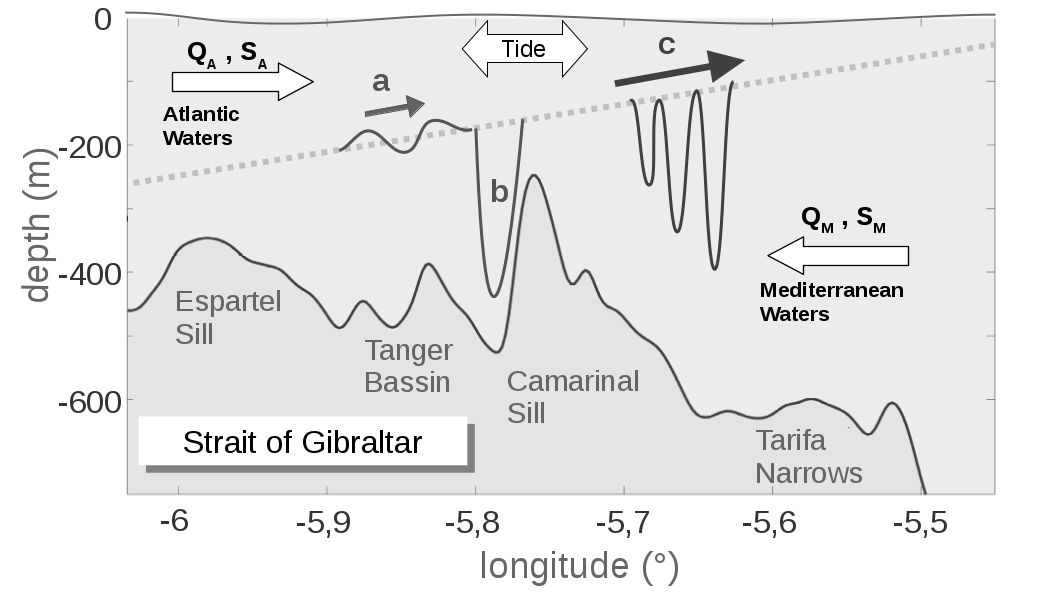
\includegraphics[width=0.51\textwidth]{./papier2D/schema_echange.png}
 \captionof{figure}{Mean exchange in the Strait of Gibraltar. The interaction of the tide with the stratification and bathymetry generates small-scale physical phenomenon. (a) Linear / Small amplitude internal wave. (b) Hydraulic Jump. (c) Large-amplitude internal waves or internal solitary waves (ISW).}
\label{scheme_GBR}
\end{wrapfigure}
%\end{figure}

Mass conservation leads indeed to : 
\begin{equation}  
	\label{Eq_mass}
    \displaystyle   
  	Q_A+Q_M = E-P
\end{equation}
and conservation of salt requires: 
\begin{equation}  
    \label{Eq_salt}
    \displaystyle   
    Q_A S_A + Q_M S_M =  0
\end{equation}
where $Q_A$ is the volume flux of Atlantic water (positive value), $Q_M$ is the volume flux of Mediterranean water (negative value) and $E-P$ is the space-averaged Evaporation minus Precipitation (and river runoff) water budget over the whole Mediterranean Sea. $E-P$ is positive. $S_A$ ($S_M$) stands for Atlantic (Mediterranean) water mean salinity and $S_M-S_A\approx 2\mbox{\textperthousand}$ (Bethoux, 1979). The excess of evaporation corresponds to a yearly averaged loss of water of about 1 meter (Garrett et al., 1990).\\

\textit{Dynamical control, maximum exchange and overmixed solution in the strait.}\\
The bathymetry of the region imposes a "dynamical control" (Baines, 1995) on the circulation in the Mediterranean basin. Such a control appears in regions of the ocean where the propagation of a particular type of waves is locally (temporally or continually) inhibited by large amplitude currents. This mechanism for the Strait of Gibraltar is illustrated in figure \ref{scheme_GBR}. In the strait, the control occurs when and where tides and water exchange generate currents with velocities larger than the velocities of the internal waves (denoted (a) in figure \ref{scheme_GBR}) propagating at the interface of Atlantic and Mediterranean waters. In the transition region a "hydraulic jump" can form (b).

Several more refined analytical models have been proposed to investigate the hydraulic control in the region of Gibraltar (Bryden and Stommel, 1984; Farmer and Armi, 1986 or Garrett et al., 1990). 
Traditionally, hydraulic controls may occur at Camarinal Sill (CS), Espartel Sill (ES), and Tarifa Narrows (TN), though the predicted location and time frequency of the appearances of these controls vary with the refinement of the model :
\begin{itemize}
\item{Farmer and Armi (1986)'s two-layer model takes into account the geometry of the strait (depth and breadth), the exchanged volumes ($Q_A$ and $Q_M$) and the salinity contrast ($S_A -S_M$). This simple model manages to predict the presence of two simultaneous hydraulic controls, one at the sill, the other at the contraction in TN, defining "maximal exchange regime"  (further details are given below). }

\item{In a slightly more elaborated model, the inclusion of the entrainment between the two layers and the subsequent introduction of a third interfacial layer modify the left-hand terms of equations (\ref{Eq_mass}) and (\ref{Eq_salt}) with the introduction of horizontal and vertical transports in this third layer (Bray, 1995). The critical conditions are also changed: new controls can in particular appear since there are now two interfaces, with potentially two baroclinic modes (Sannino et al., 2009).}

\item{ When now considering a three-dimensional flow, the definition of the control needs to integrate cross-strait variations such as the tilt of the interface in this direction (Sannino et al, 2009). In the maximal exchange solution, control in TN can for instance result in the detachment of the surface layer from the northern shore.}
\end{itemize}

These conditions on the flow, when combined with the above two conservation equations (\ref{Eq_mass}) and (\ref{Eq_salt}), can be used to relate volume fluxes and evaporation with the input salinity difference ($S_A-S_M$). As a consequence, local characteristics of the exchange flow in the Strait of Gibraltar can be linked to the formation of Mediterranean waters (Bryden and Stommel, 1984) and to the diapycnal mixing over the Mediterranean basin. The "overmixed solution" corresponds in this case to a minimal salinity difference and to a maximal exchange of mass.

In-situ observations suggest that this maximal exchange is attained only punctually in the strait during the year, the rest of the time the exchange is called "submaximal". Tidal currents impose a strong signature on this complex mechanism of hydraulic control in the strait at different timescales ranging from the tidal cycle to the neap/spring tidal modulation. Seasonal lower frequency can also change the occurrence and the locations of the hydraulic jumps.\\

\textit{Internal Solitary Waves.}\\
Those hydraulic jumps are large-amplitude depressions in the regions of hydraulic controls. There, intense mixing occurs between the Atlantic and Mediterranean waters, changing for example the characteristics of the Mediterranean outflow, which is one seasonal component of the circulation in the Northern Atlantic. 

The relaxation of those jumps generates large-amplitude, non-linear, non-hydrostatic trains of Internal Solitary Waves (ISW) (denoted (c) in figure \ref{scheme_GBR}). When the barotropic tide is constrained by the bathymetry of the strait, large vertical velocities appear and energy is transmitted to several normal modes of internal waves. In the Strait of Gibraltar, the largest amplitude ISW observed correspond to the first baroclinic mode (no change of direction of the induced velocity through the water column, all isopycnal surfaces are in phase). The signature of Modes 2 waves (vertical velocity profile showing one node, spreading of the isopycnals) has also been observed in the region of Gibraltar strait (Farmer and Armi, 1988, V\'azquez and al, 2006).

These waves propagate at the interface of Mediterranean and Atlantic water layers. In addition to their unknown impact on the local and remote mixing of the Atlantic and Mediterranean waters, the correct forecast of the generation and propagation of these peculiar waves still remains a challenge. \\

\textit{Consequences on basin-scale circulation.}\\
The region of the strait is thus relevant not only for its own dynamic and for the resulting peculiar turbulent cascade but also for its impact on both the outflowing Mediterranean and inflowing Atlantic waters. Indeed the various small-scale processes described above modify the characteristics of Atlantic and Mediterranean waters and, down the line, their behavior as they circulate respectively in the Mediterranean and in the Northern Atlantic.

To study these consequences in greater depth, numerical modeling is required. Some rudimentary models of the strait have for instance been achieved by modeling specifically the two layers of Atlantic and Mediterranean waters (Brandt 1996; Izquierdo 2001). With the increase in computational power, 3D modeling with greater vertical and horizontal sampling are feasible (Sannino et al., 2004). The tidal cycle and some features of the flow can be simulated. Several non-hydrostatic models have then been proposed (Sanchez Garrido, 2011; Sannino, 2014), which allows the representation of ISW. Other configurations include the strait of Gibraltar into a Mediterranean circulation model (Soto Navarro et al., 2014). Enhanced resolution in the strait (Naranjo et al., 2015) or nesting of a high-resolution grid of the strait in a lower-resolution model of the Mediterranean (Sannino et al., 2009) impact the stratification in the Mediterranean and improve the representation of convective events in the Gulf of Lion.\\
Lately, a new non-hydrostatic regional ocean model has been proposed (Auclair et al., 2018). It is based on regional ocean models (Symphonie in a research, Leap-Frog, 3-mode version and lately ROMS-CROCO in an efficient, LF-AM3, 2-mode version) in which the incompressible (Boussinesq-flow) assumption is relaxed together with the hydrostatic assumption. This new model opens new perspectives in terms of modeling of small-scale processes since Navier-Stokes equations can be simulated with much less restrictive numerical assumptions whereas computing costs have been drastically reduced following Shchepetkin and McWilliams (2005) advanced numerical technics.\\

% \\
%\textit{\textbf{What are the objectives of the present study ?}} \\

\textit{Objectives of the present study.}\\
The objectives of the present study are both numerical and physical. We show that a new generation of non-hydrostatic ocean models can be used to forecast complex non-linear, non-hydrostatic physics in a realistic, easy-to-implement and computationally-affordable configuration. The complete set of Navier-Stokes equations is integrated in time and it is presented for the very first time in such a complex region as Gibraltar.\\
The now-classical but still numerically-demanding chosen configuration is based on a lock-exchange initialization (Sannino et al., 2002). To the author knowledge, the present configuration can also be viewed as one of the very first (M)ILES\footnote{Monotonic implicit large eddy simulation \color{black}} model (Grinstein et al., 2007) of the region of Gibraltar. 
A 2D vertical subsection of the strait has been chosen in order to reduce the number of parameters having an impact on the studied dynamics. As such, the vertical subsection appears as an exploratory study preparing the implementation of a more complex fully 3D model in the studied region. In an obvious way, a 2D-vertical subsection is implemented firstly to reduce the computational cost and implementation burden. This leads us to propose an easy-to-implement and computationally-affordable tool that can be run in various contexts.\\

%\color{blue} A partir de là, il faudrait indiquer les subsections dans lesquelles sont détaillés les points cités (et au besoin la réorganiser un peu dans l'ordre chronologique. \color{black}.\\

In subsection 2 we give a review of the CROCO-NBQ model dynamics and we present the implementation of the 2D lock-exchange experiment. We carefully discuss and evaluate the way the bathymetry profile, the water masses, the exchange and tidal flows can be integrated in a forecasting system. In subsection 3 we evaluate the physics of the 2D configuration. In subsubsection 3.1 we compare the forecasted dynamics to published data such as in Farmer and Armi (1988), with emphasis on hydraulic controls, hydraulic jumps and mode-1 and mode-2 ISW (non-linear internal trains of solitary wave) propgation. The dispersion and damping of the train of mode 1 solitons as it propagates over the deeper eastern side of the strait is studied in subsubsection 3.2. To this aim, we compare the forecast with the Extended Korteweg-de Vries (eKdV) equation and with satellite images. Finally, both physical (topography, tidal amplitude) and numerical (spatial resolution, non-hydrostatic algorithm) sensitivity-tests are carried out respectively in subsections \ref{TestPhy} and \ref{TestNum}, with a focus on the changes on the fine-scales dynamics listed in figure \ref{scheme_GBR}.

%We investigate the dynamics of hydraulic jumps in areas of hydraulic controls. Modes 1 and 2 of non-linear internal trains of solitary wave are carefully studied and their forecast is compared to published data from Gibraltar Experiment (Army and Farmer, 1988). The region and date of generation and propagation of both modes are more particularly addressed. The propagation of the train of Mode-1 solitons over the deeper eastern side of the strait is then studied.

%Both numerical and physical sensitivity-tests are finally carried out. The advection of internal modes by the tidal current is also discussed. The dispersion and damping of the train of solitons are discussed and the model is compared with the Modified Korteweg-de Vries (KdV) equation and with satellite images.
% Based on this realistic configuration the forecasting capabilities of the model are finally more specifically evaluated.\\
% \\
% \textit{\textbf{Why did we choose a numerical configuration based on a 2D vertical subsection with a yet fully 3D ocean-model?}}


%We however have to make sure that the physics of the 2D subsection remains realistic and that the restriction to a  vertical subsection does not lead to specific unrealistic mechanisms.

%%%%%%%%%%%%%%%%%%%%%%%%%%%%%%%%%%%%%%%%%%%%%%%%%%%%%%%%%%%%%%%%%%%%%%%%%%%%%
\subsection{Numerical configuration}
%%%%%%%%%%%%%%%%%%%%%%%%%%%%%%%%%%%%%%%%%%%%%%%%%%%%%%%%%%%%%%%%%%%%%%%%%%%%%

%----------------------------------------------------------------------------
\paragraph{The numerical forecasting system}
%----------------------------------------------------------------------------

%\indent In the region of Gibraltar, the Atlantic inflow and Mediterranean outflow circulations and the barotropic tidal waves interact with the narrow and shallow (less than 1 km deep) topography of the strait. Hydraulic jumps, non-linear internal waves, small-scale shear instabilities... are generated in the region of the strait leading to very energetic fine scale dynamics. \color{blue} L'introduction de cette partie est peu longue car tu as déjà traité tout cela dans la subsection précédente. \color{black}.

The proposed numerical model of the Strait of Gibraltar simulates explicitly the fine-scale processes (from tens to hundreds of meters) discussed previously. This means that (i) a sufficient grid resolution must be provided in the strait and (ii) a dedicated numerical kernel must be used.

The non-hydrostatic (non-Boussinesq) version of the CROCO community ocean model (CROCO- NBQ) is thus chosen for his ability to allow LES\footnote{LES (Large Eddy Simulation): LES, in contrast to DNS (Direct Numerical Simulation) does not simulate the full 3D Kolmokorov-like energy cascade down to molecular scales. However at least the onset of this cascade is explicitly represented unlike in RANS (Reynolds Averaged Navier-Stokes).} and it is implemented in a realistic configuration in order to evaluate its capacity to forecast complex non-hydrostatic dynamics in an easy-to-implement configuration. In LES, the direct transfer ends at the lowest scale resolved, and subgrid dissipation of energy is accomplished by implicit mixing of the advective scheme, as well as by explicit parametrisation.

The regional ocean model CROCO-NBQ is an extension of ROMS from which it inherited the robustness and efficiency of the time-splitting (Shchepetkin and McWilliams, 2005 , Debreu et al, 2012). CROCO-NBQ is based on a time-splitting algorithm: the numerics of the "slow" mode is similar as ROMS internal mode (Shchepetkin and McWilliams, 2005) whereas the "fast mode" has lately been adapted to include both the "External mode" and the evolution of the s-grid of ROMS-AGRIF together with an evolution of the non-hydrostatic and non-Boussinesq kernel of Symphony-NBQ model (Auclair et al., 2018). A two-mode time-splitting kernel is conserved but if the slower, internal mode, is only slightly modified by introducing a prognostic calculus of vertical momentum, the fast mode (once barotropic) now deals with a 3D-compressible flow. \\

 %----------------------------------------------------------------------------
 \paragraph{Continuous free-surface compressible equations in z-coordinates}
 \label{NavierStokes}
 %----------------------------------------------------------------------------
 
\indent The full set of Navier-Stokes equations for a free-surface ocean is explicitly integrated and the continuity and momentum equations, the surface kinematic relation, the heat, salt and state equations respectively read in Cartesian coordinates: 
\begin{alignat}{2}
  \displaystyle
   %%%%%%%%%%%%%%%%%%%%%%%%%%%%%%%%%%%%%%%%%%%%%%
   % Continuity
   %%%%%%%%%%%%%%%%%%%%%%%%%%%%%%%%%%%%%%%%%%%%%%
   &\partial_t\rho &&=-\vec{\nabla}.(\rho\vec{v})\\[3mm]
   %%%%%%%%%%%%%%%%%%%%%%%%%%%%%%%%%%%%%%%%%%%%%%
   % Momentum
   %%%%%%%%%%%%%%%%%%%%%%%%%%%%%%%%%%%%%%%%%%%%%%
   \label{momentum}
   &\partial_t\rho\vec{v} &&=
   -\vec{\nabla}.\left(\rho\vec{v}\otimes\vec{v}\right)
   -2\rho\vec{\Omega}\wedge\vec{v}
   -\vec\nabla p+\rho\vec{g}
   +\mu\Delta\vec{v}
   +\lambda\vec{\nabla}(\vec{\nabla}.\vec{v})\\[3mm]
   %%%%%%%%%%%%%%%%%%%%%%%%%%%%%%%%%%%%%%%%%%%%%%
   % Surface kinematic relation
   %%%%%%%%%%%%%%%%%%%%%%%%%%%%%%%%%%%%%%%%%%%%%%
   &\partial_t{\zeta} &&= 
   w\scriptstyle(z=\zeta)\textstyle
   -\vec{v}\scriptstyle(z=\zeta)\textstyle.\vec{\nabla}{\zeta}\\[3mm]
   %%%%%%%%%%%%%%%%%%%%%%%%%%%%%%%%%%%%%%%%%%%%%%
   % Heat equation
   %%%%%%%%%%%%%%%%%%%%%%%%%%%%%%%%%%%%%%%%%%%%%%
   &\partial_t{\rho\theta} &&=-\vec{\nabla}.\left(\rho\theta\vec{v}\right)
   +\kappa_{\theta}\Delta\theta\\[3mm]
   %%%%%%%%%%%%%%%%%%%%%%%%%%%%%%%%%%%%%%%%%%%%%%
   % Salt equation
   %%%%%%%%%%%%%%%%%%%%%%%%%%%%%%%%%%%%%%%%%%%%%%
   &\partial_t{\rho s} &&=-\vec{\nabla}.\left(\rho s\vec{v}\right)
   +\kappa_{s}\Delta s\\[3mm]
   %%%%%%%%%%%%%%%%%%%%%%%%%%%%%%%%%%%%%%%%%%%%%%
   % State equation
   %%%%%%%%%%%%%%%%%%%%%%%%%%%%%%%%%%%%%%%%%%%%%%
   &\rho &&=\varrho\left(\theta,s,P\right)
\end{alignat}
where $\vec{v}=(u,v,w)$ is the velocity, $p$ the total pressure, $\zeta$ the free-surface anomaly $\rho$ the density, $\theta$ and s respectively the potential temperature and salinity. $\vec{\Omega}$ is the instantaneous earth rotation vector, $\vec{g}$ is the acceleration of gravity and $\mu$, $\lambda$, $\kappa_{\theta}$ and $\kappa_{s}$ are respectively the dynamical and second (bulk) viscosity and the thermal and salinity diffusivities.

   
 %----------------------------------------------------------------------------  
 \paragraph{Density and pressure decomposition}
 %----------------------------------------------------------------------------
\indent To allow ROMS-like time-splitting, density is decomposed into slow and fast components based on a first-order decomposition with respect to total pressure. In the following, s and f subscripts respectively refer to slow and fast-mode components.\\
\begin{alignat}{2}
  \displaystyle
   %%%%%%%%%%%%%%%%%%%%%%%%%%%%%%%%%%%%%%%%%%%%%%
   % Density
   %%%%%%%%%%%%%%%%%%%%%%%%%%%%%%%%%%%%%%%%%%%%%%
  &\rho &&=\rho_{s}\left(\theta,s,P\right)
  +\overbrace{\left.{\frac{\partial{\rho}}{\partial{P}}}\right|_{\theta,s}\delta{P}}^{\delta{\rho}=\rho_{f}}
  +O\left(\delta{P}^2\right)\\
   %%%%%%%%%%%%%%%%%%%%%%%%%%%%%%%%%%%%%%%%%%%%%%
   % Pressure
   %%%%%%%%%%%%%%%%%%%%%%%%%%%%%%%%%%%%%%%%%%%%%%
  &P &&=\underbrace{P_{atm}
  +\int\limits_z^{\zeta}{(\rho_{s}-\rho_0)g\ dz'}}_{Slow\ mode}
  +\underbrace{\rho_{0}g(\zeta-z)+\underbrace{\delta P}_{P_{f}}}_{Fast\ mode}
\end{alignat}
  
No further decomposition is required for other variables.
  
 
%----------------------------------------------------------------------------  
 \paragraph{Slow vs fast components}
 %----------------------------------------------------------------------------
\indent Navier-Stokes equations are consequently integrated with two different time-steps in a time-splitting algorithm. The slow mode is identical to ROMS slow "internal" mode whereas the fast-mode (unlike in ROMS) is 3D and allows the integration of the compressible terms of the momentum and continuity equations and of the free-surface anomaly through the free-surface kinematic condition.
\begin{equation}
  \begin{split}
  %\begin{equation}
    \displaystyle
   %%%%%%%%%%%%%%%%%%%%%%%%%%%%%%%%%%%%%%%%%%%%%%
   % Continuity
   %%%%%%%%%%%%%%%%%%%%%%%%%%%%%%%%%%%%%%%%%%%%%%
   &\partial_t\ \rho_f &= -\partial_t\ \rho_{s}
   &-\vec{\nabla}.(\rho\vec{v})\\
   %%%%%%%%%%%%%%%%%%%%%%%%%%%%%%%%%%%%%%%%%%%%%%
   % Momentum
   %%%%%%%%%%%%%%%%%%%%%%%%%%%%%%%%%%%%%%%%%%%%%%
   &\partial_t\rho\vec{v} &= 
   & \overbrace{-\vec{\nabla}.\left(\rho\vec{v}\otimes\vec{v}\right)
   -2\rho\vec{\Omega}\wedge\vec{v}
   -\vec\nabla(\int\limits_z^{\zeta_f}{(\rho_{s}-\rho_0)g\ dz'})
   +\mu\Delta\vec{v}}^{\vec{\Lambda}_{s}}\\
   & & &\underbrace{-\rho_{0}g\vec\nabla\zeta_f
   -\vec\nabla{P}
   +\rho\vec{g}
   +\lambda\vec{\nabla}(\vec{\nabla}.\vec{v})}_{\vec{\Lambda}_{f}}\\
   %%%%%%%%%%%%%%%%%%%%%%%%%%%%%%%%%%%%%%%%%%%%%%
   % Surface kinematic relation
   %%%%%%%%%%%%%%%%%%%%%%%%%%%%%%%%%%%%%%%%%%%%%%
.   &\partial_t{\zeta_f} &&= 
   w_f\scriptstyle(z=\zeta)\textstyle
   -\vec{v_f}\scriptstyle(z=\zeta)\textstyle.\vec{\nabla}{\zeta_f}\\[3mm]
   %%%%%%%%%%%%%%%%%%%%%%%%%%%%%%%%%%%%%%%%%%%%%%
   % Heat equation
   %%%%%%%%%%%%%%%%%%%%%%%%%%%%%%%%%%%%%%%%%%%%%%
   &\partial_t{\rho\theta_s} &=\ &\Theta_{s}=-\vec{\nabla}.\left(\rho\theta_s\vec{v}\right)
   +\kappa_{\theta}\Delta\theta_s\\
   %%%%%%%%%%%%%%%%%%%%%%%%%%%%%%%%%%%%%%%%%%%%%%
   % Salt equation
   %%%%%%%%%%%%%%%%%%%%%%%%%%%%%%%%%%%%%%%%%%%%%%
   &\partial_t{\rho s_s} &= &\ S_{s}= -\vec{\nabla}.(\rho s_s\vec{v})
   +\kappa_{s}\Delta{s_s}\\
   %%%%%%%%%%%%%%%%%%%%%%%%%%%%%%%%%%%%%%%%%%%%%%
   %State equations
   %%%%%%%%%%%%%%%%%%%%%%%%%%%%%%%%%%%%%%%%%%%%%%
   &\rho_s &= &\varrho(\theta_s,s_s,\zeta_f)\\
   &\rho_f &= &c_s^{-2} P_f
  \end{split}
\end{equation}
  
No indice is specified for momentum since this variable is integrated both in slow and fast modes. Slow (fast) prognostic equations and diagnostic relations are respectively integrated in slow (fast) mode. Momentum equations are integrated in both modes. More details can be found in Auclair et al. (2018).

%----------------------------------------------------------------------------  
 \paragraph{Bathymetry of the numerical configuration}
 \label{BathyNum}
 %----------------------------------------------------------------------------
%%%%%%%%%%%%
% Figure 1
%%%%%%%%%%%%
\begin{figure}[!h]
\centering
 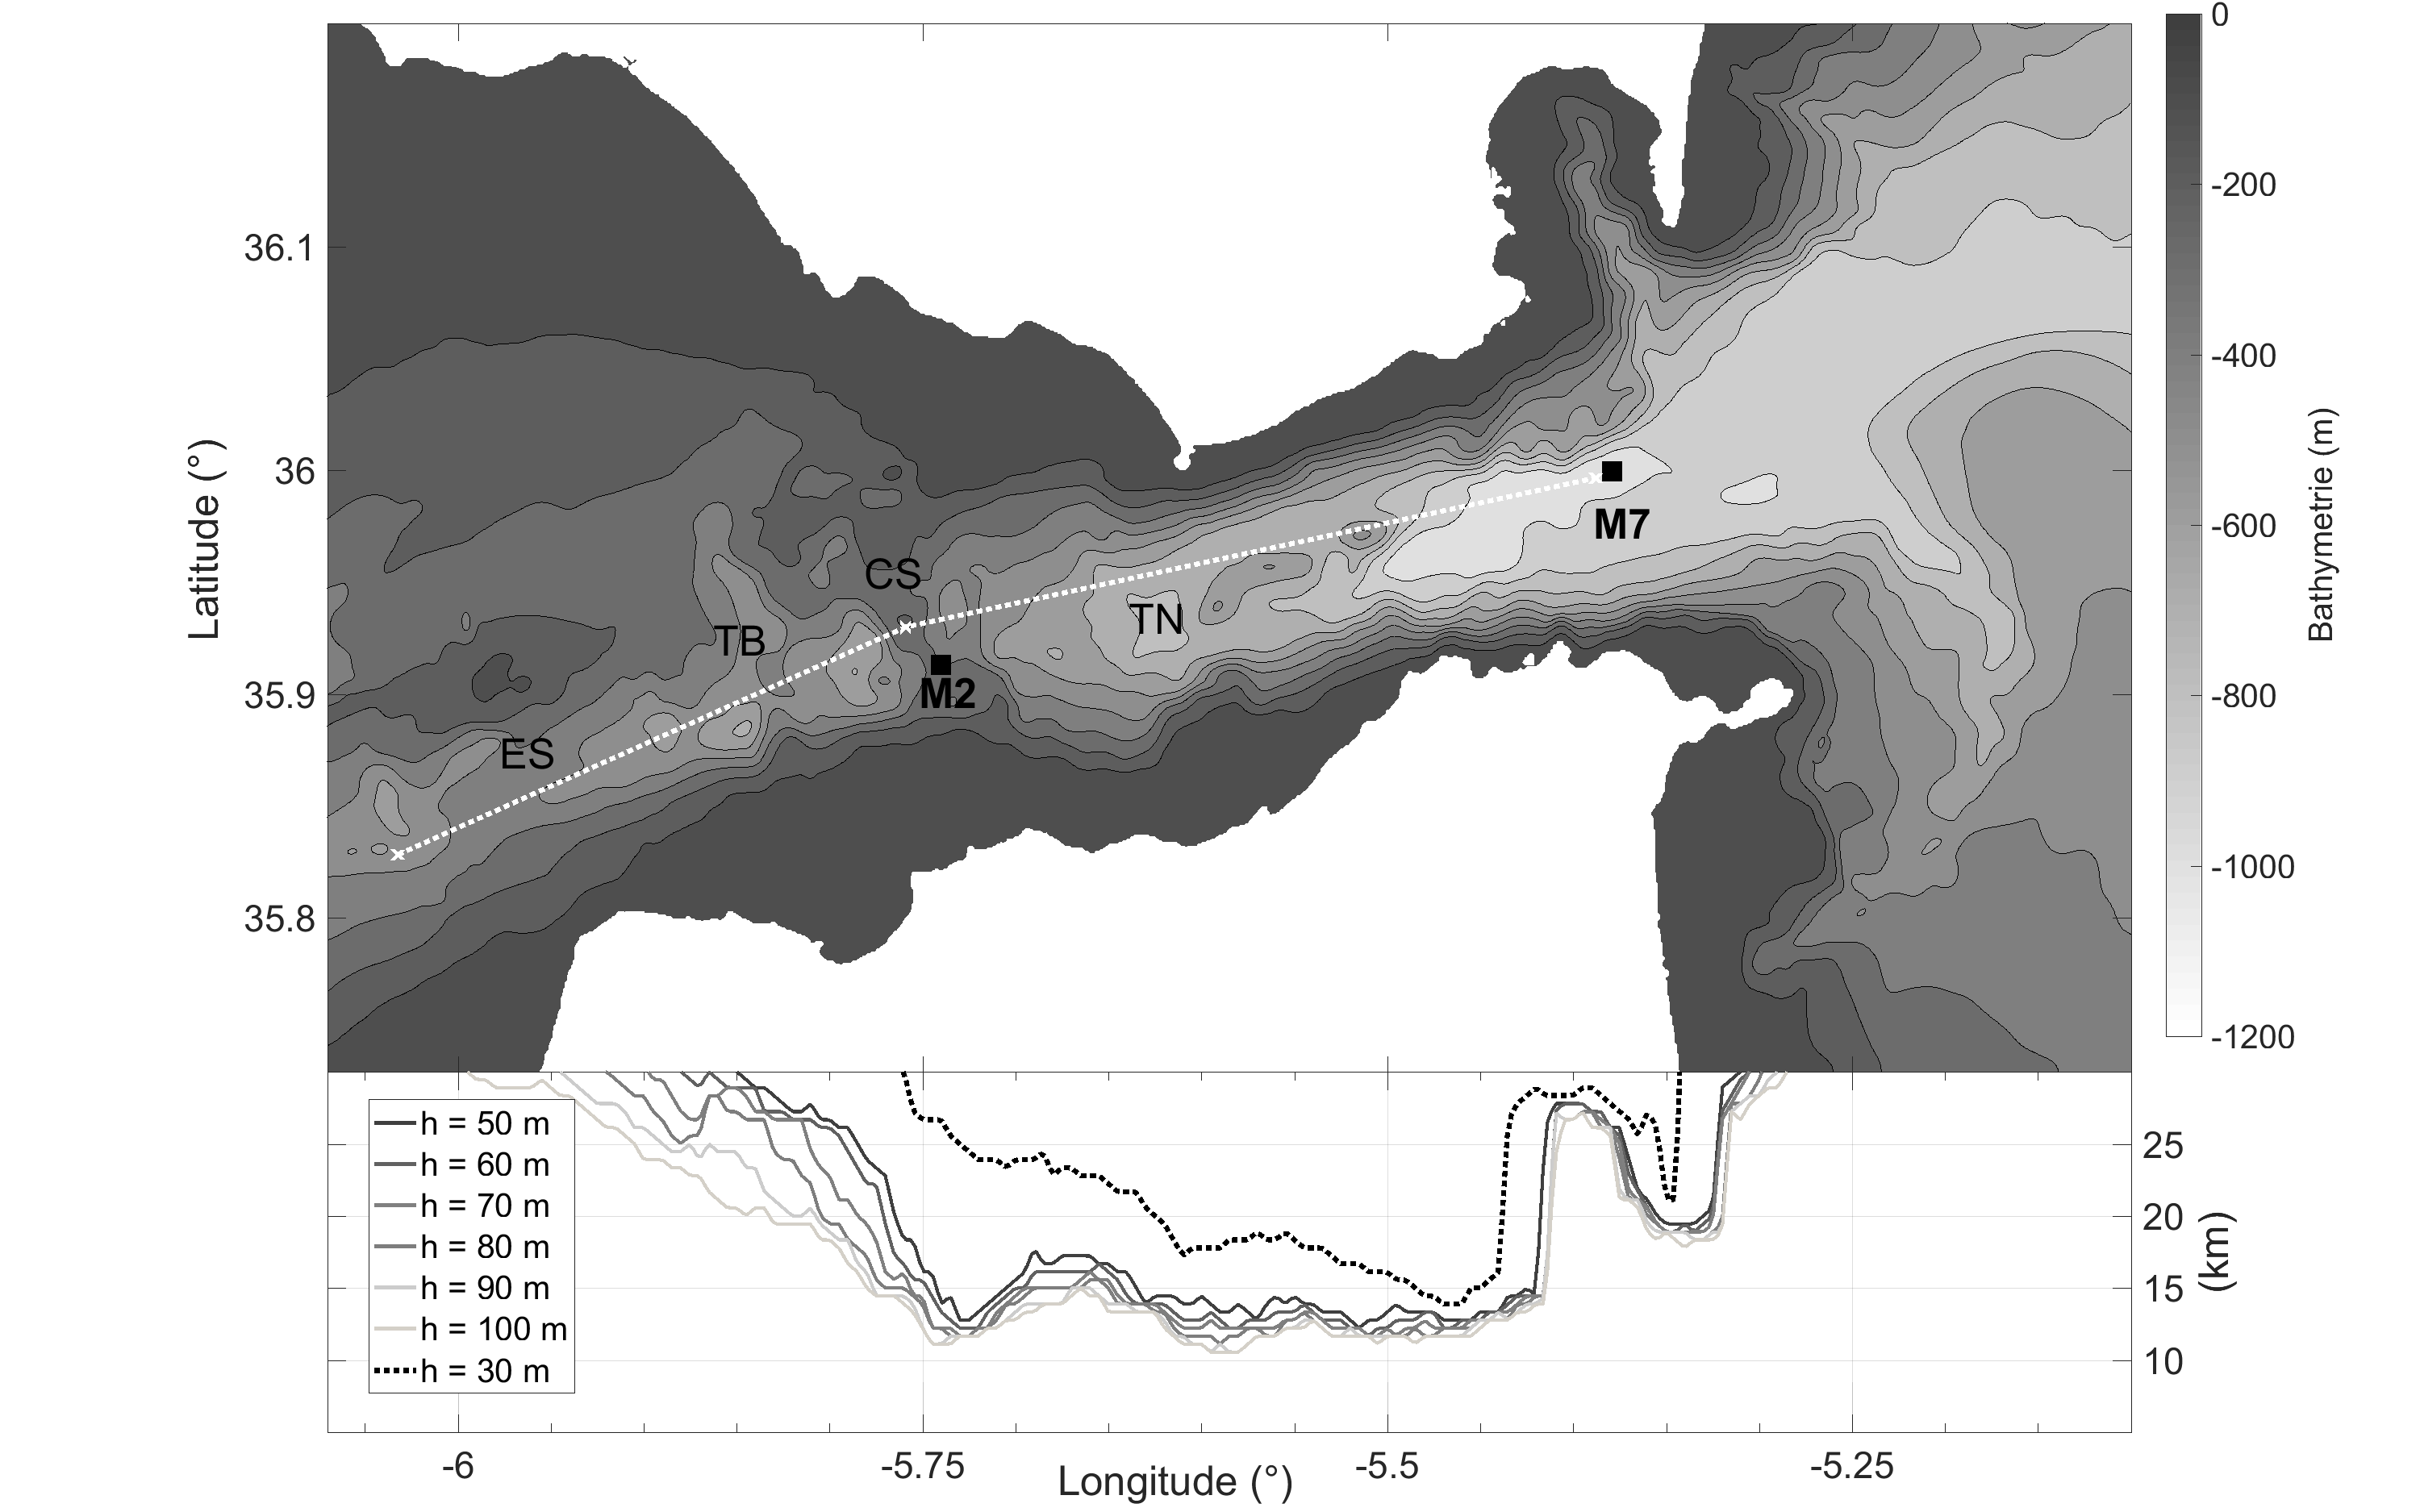
\includegraphics[width=1\textwidth]{./papier2D/bathy3d+Rr3d.png}
 \caption { a) Bathymetry of the strait of Gibraltar, location of the transect A (white dotted line). Black squares indicate the position of moorings. (ES: Espartell Sill, TB: Tanger Basin, CS: Camarinal Sill , TN: Tarifa Narrows)
 b) Maximum distance along the transverse (y) direction between 2 isobaths of depth h.}
 \label{Fig1}
\end{figure}

\indent In figure \ref{Fig1}.a is depicted the 500 m-resolution bathymetry developped in the framework of the HOMONIM project coordinated by the French Navy (SHOM) and MeteoFrance as provided by the French Navy, with the  principal geographical features as well as the localization of the studied vertical 2D subsection. This subsection is chosen as close as possible to the transect of Farmer and Armi's Gibraltar Experiment realized in April 1986 (Farmer and Armi, 1988). Hereafter, $u$ is defined as the velocity in the longitudinal direction and $v$ the velocity in the transverse direction. Figure \ref{Fig1}.b presents the width of the Strait of Gibraltar relative to different reference depths. This plot indicates that an averaged strait width of approximately 13 km can be chosen, evidencing the steep slopes at the lateral boundaries of the straits, especially in Tarifa Narrows.

Simulations are successively achieved with horizontal resolutions of 220 m and then 50 m. So as to limit the unrealistic effect of punctual seamounts in the transverse direction such as those found in TN (which can, in a vertical 2D subsection, end up acting as another sill), a Gaussian interpolation of the bathymetry is provided with a greater Gaussian radius in the transverse direction than in the longitudinal direction. In the following, the Gaussian radius in the transverse direction is chosen equal to 1500 m (ie. inferior to the width of the strait in figure \ref{Fig1}.b). As a consequence, the bathymetry only reflects the deepest areas in the canal. 
%corresponds approximately to half the width of the 1000-m deep canal in the region of TN. 
In the longitudinal direction, the Gaussian interpolation radius is only 300 m to preserve bathymetry variability in this direction.

Using this method to interpolate bathymetry, the minimum depth at Camarinal Sill, the main sill of the Strait of Gibraltar, goes from the real value of approximately 200 m to 247.6 m. Further characteristics of the reference forecast based on this bathymetry (hereafter named \textbf{SimRef}) are presented in table \ref{tabsimref}.\\

%--------------------------------
\paragraph{Water mass and tidal forcing}
%--------------------------------
\indent Realistic forecasts of limited-area domains require at least temperature and salinity profiles in the studied region and, as a consequence, they are not easy to initialize nor to constrain at their open boundaries. A minimum number of two profiles is needed to initialize gradients associated to sloping isopycnal surfaces in a given direction. Following Sannino et al. (2002), a lock-exchange initialization of the region of the strait can be implemented with Atlantic water on the western side of CS and Mediterranean water on the eastern side at t = 0 s. A three-day period of simulation (spin-up phase) is then achieved to set up the exchange flow in the strait.

The initial temperature and salinity profiles are presented in figure \ref{fig_LEx}, where we see a contrast in salinity between Atlantic and Mediterranean water, with respective mean of 35.9 and 38.2. In the following, the interface between the Atlantic and Mediterranean layers in terms of salinity is chosen as the 37 isohaline (Bryden, 1994). Density is now expressed as an anomaly (written $\rho'$) relative to a reference density $\rho_{0}$ computed by the model. In the following, if not specifically specified,the reference density is $\rho_{0}=1033.7$ kg/m$^3$.

The M2 tidal forcing (of period T = 12.4 h) is activated only after the spin-up period. It is simulated by a barotropic current of amplitude 0.4 m/s at the western boundary (0.8 m/s at CS). This corresponds to a neap-tide regime in the TPXO-8 tidal atlas (Egbert and Erofeeva, 2002).

\vspace{1\baselineskip}
\begin{minipage}{.4\textwidth}
%\begin{table}
\centering
\begin{tabular}{|p{\linewidth/3}|c|c|}
\hline
Number of horizontal points & \multicolumn{2}{c|} {602x3}  \\
%\hline
$\Delta x$ & \multicolumn{2}{c|} {221 m}\\ 
%\hline
Number of $\sigma$-levels & \multicolumn{2}{c|} {40} \\
%\hline
Depth & Min & Max\\
%\cline{2-3}
   & 247.6 m & 900 m\\
%   \hline
   $\Delta$z & 6 m & 23 m\\
%\hline
$\Delta t_s$ & \multicolumn{2}{c|} {4 s}\\
%\hline
$\Delta t_f$ & \multicolumn{2}{c|} {0.5 s}\\
%\hline
Vertical Viscosity & \multicolumn{2}{c|} {$10^{-6}$ m$^2$/s}\\
%\hline
Lateral Viscosity & \multicolumn{2}{c|} {$10^{-5}$ m$^2$/s}\\
%\hline
Diffusivity & \multicolumn{2}{c|} {$10^{-6}$ m$^2$/s}\\
%\hline
Momentum Advective Scheme & \multicolumn{2}{c|} {TVD}  \\
%\hline
TS Advective Scheme & \multicolumn{2}{c|} {WENO5}  \\
\hline
\end{tabular}
\captionof{table}{Numerical parameters of simulation \textbf{SimRef}}
\label{tabsimref}
\end{minipage}
%\end{table}
 ~
\begin{minipage}{.4\textwidth}\centering
%\begin{figure}[!t]
 \centering
 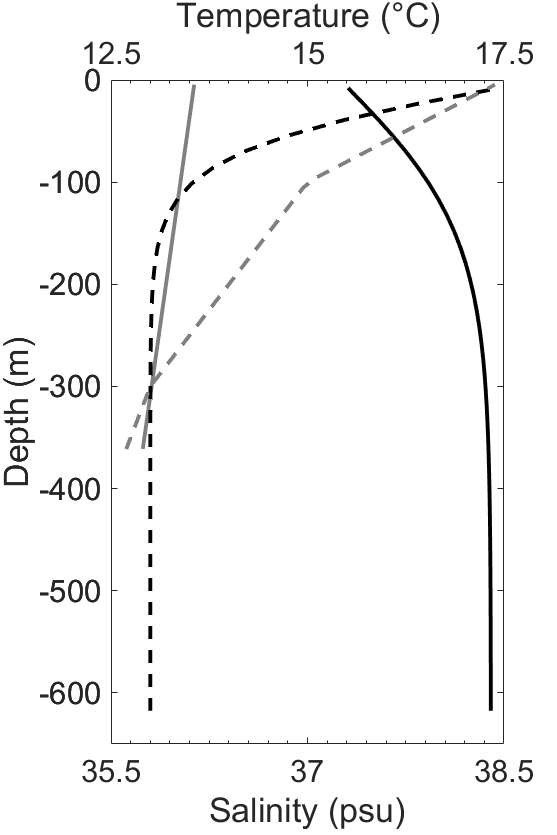
\includegraphics[width=\linewidth]{./papier2D/profil_LEx.png}
 \captionof{figure} {Salinity and temperature (dashed lines) profile of Mediterranean water (red) and Atlantic water (blue) at initial time-step}
\label{fig_LEx}
%\end{figure}
\end{minipage}
\vspace{1\baselineskip}



% ~
%%\begin{minipage}{.6\textwidth}\centering
%\begin{figure}[!t]
% \centering
% 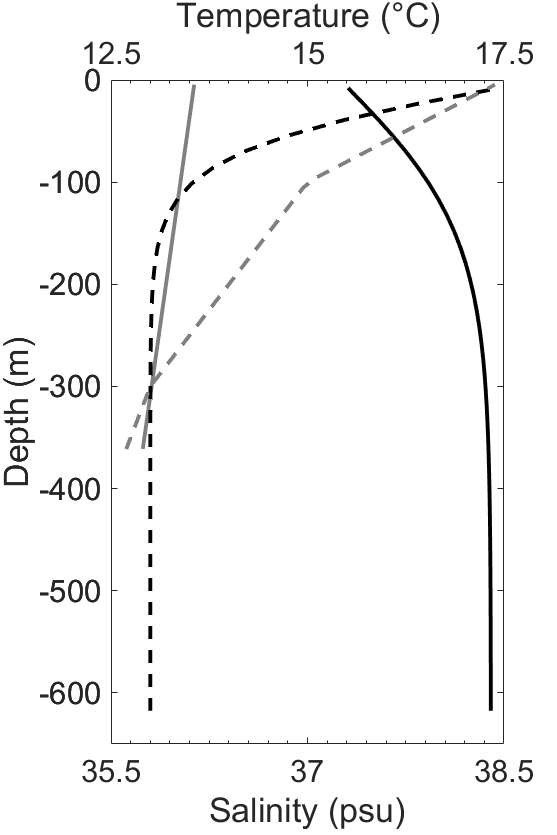
\includegraphics[width=0.6\textwidth]{./papier2D/profil_LEx.png}
% \captionof{figure} {Salinity and temperature (dashed lines) profile of Mediterranean water (black) and Atlantic water (grey) at initial time-step}
%\label{fig_LEx}
%\end{figure}
%%\end{minipage}


 
%----------------------------------------------------------------------------
\paragraph{Initialization of density profile and shear current : effect of Coriolis Pseudo-Force}
\label{Coriolis}
%----------------------------------------------------------------------------

The lateral boundaries of the strait of Gibraltar are distant of about 15 km, with a clear funneling effect from CS to the end of the strait when looking at subsurface isobaths (see figure \ref{Fig1}.b). The internal Rossby radius $R={\sqrt{g'h}}/{f}$ is usually observed as varying between 10 and 20 km (Bormans and Garrett 1989, Candela 1990, Vlasenko and al 2009). Here $g'= g (\rho_M(S_M) - \rho_A(S_A))/\rho_0$ is the reduced gravity, $h=h_1 h_2/(h_1+h_2)$ is a characteristic height with $h_1$ and $h_2$ respectively the upper and lower layer thicknesses, and $f$ is the Coriolis parameter. The width of the strait and $R$ are of the same order, indicating that rotational effects due for instance to geostrophy can be neglected as a first approximation. 

Hence, the balance is mainly between acceleration and the pressure force in equation (\ref{momentum}) and geostrophic adjustment in the along-strait direction is locally neglected. In observations (Farmer and Armi, 1988) and 3D-modeling configuration (Saninno, 2002), the consequences of Earth's rotation are a cross-strait shear of along-strait velocity (Bormans and Garett, 1989) and a tilt of the interface between Mediterranean and Atlantic waters, with greater velocities and a deeper interface along the southern (Moroccan) coast.

%
%%%%%%%%%%%%
% Figure 
%%%%%%%%%%%%
\begin{figure}[!t]
 \centering
 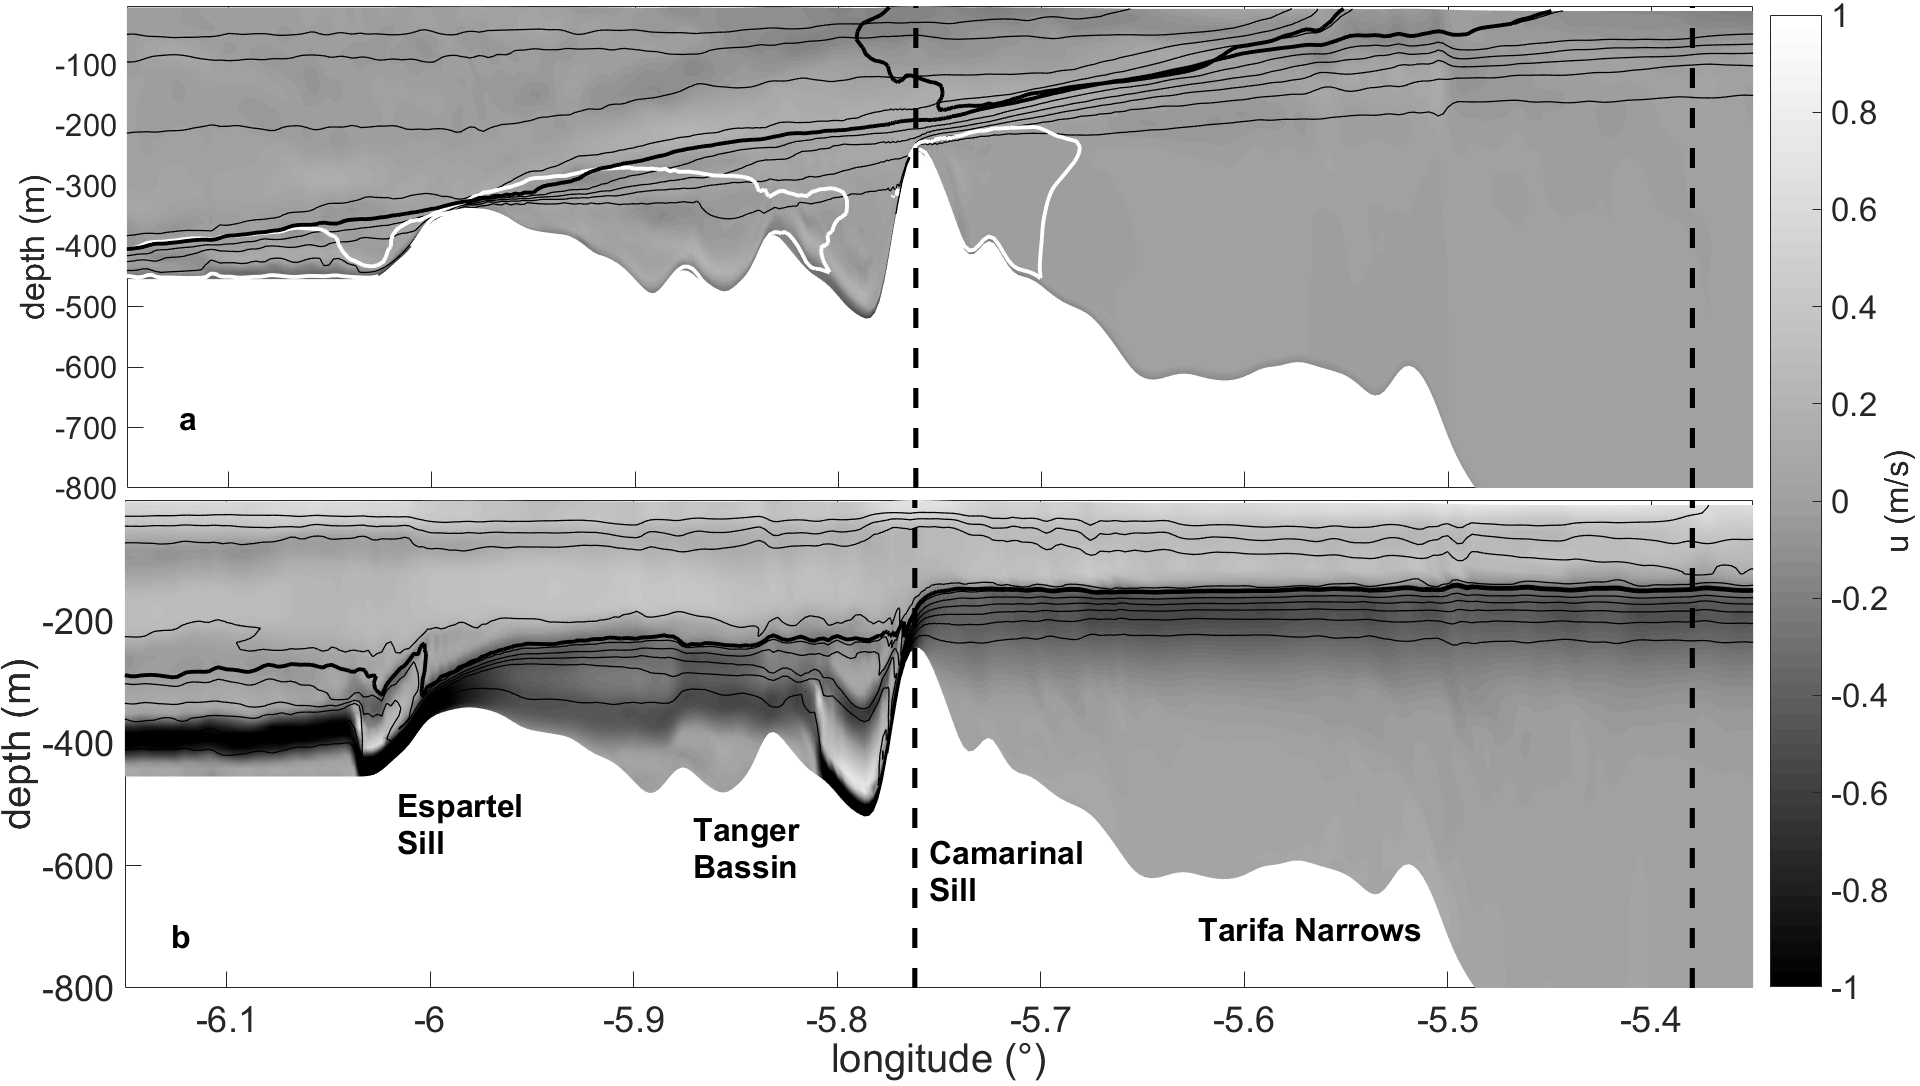
\includegraphics[width=1\textwidth]{./papier2D/stratif_corio_vs_nocorio.png}
 \caption {Longitudinal current and isopycnal contours at 70 h during the spin-up phase for \textbf{SimAllCor} (a) and \textbf{SimNoCor} (b).
 White contour : transversal current $v = 0.5 \ m/s$  Black contour : transversal current v=-0.5 \ m/s. Bolded isopycnal $\rho' = -0.7 \ kg/m^3$.
 The vertical dashed lines indicate the location of the profiles given in figure \ref{fig_current}.}
  \label{fig2}
\end{figure}
The transverse flow, the lateral boundaries and the resulting ``funeling effect'' cannot be simulated in a 2D vertical subsection, and we consequently need to examine how this limitation impacts both the stratification and the mean circulation. For this, we compare the initialization of a simulation with (i) the Coriolis pseudo-force activated from start to end (\textbf{SimAllCor}) ($f = 8.5 \ 10^{-5} s^{-1}$), (ii) a simulation without the Coriolis pseudo-force (the Coriolis parameter is set to zero) (\textbf{SimNoCor}), and (iii) a simulation with the Coriolis pseudo-force activated only after the spin-up period (\textbf{SimRef}). Apart from the choice of Coriolis parameter, the three simulated vertical subsections have the characteristics given in table \ref{tabsimref} for \textbf{SimRef}.

During the very first hours of simulations, the 'Lock-Exchange dam' separating the Atlantic and Mediterranean water-masses disappears, a gravity current is generated with dense Mediterranean waters flowing down the slope of CS and light Atlantic water spreading in the surface layer.
%\afterpage{
%%%%%%%%%%%
% Figure 
%%%%%%%%%%% 
%\begin{figure}[!t]
%\centering
%\includegraphics[width=\textwidth]{comp_UV_M.png}
%\caption {Mean zonal current (blue) and meridional current (red) above CS averaged over 3T at stations M2 and M7 for configurations %\textbf{SimAllCor} and \textbf{SimNoCor}(right). Locations of profile are given in Figure \ref{fig2}.}
%\label{fig_current}
%\end{figure} 


\begin{minipage}{0.45\textwidth}
%\begin{figure}
  \centering
  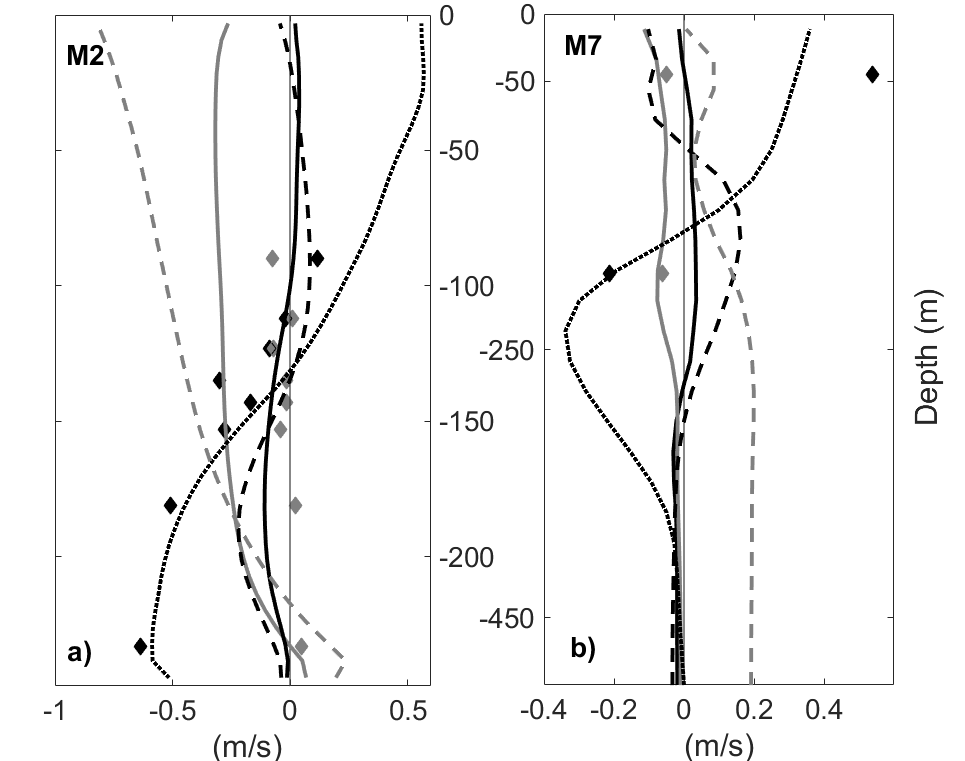
\includegraphics[width=\textwidth]{./papier2D/UV_CS_3T_ref.png}
  \captionof{figure}{3T-averaged longitudinal (black) and transversal current (grey) at the locations in figure \ref{fig2} for configurations \textbf{SimRef} (plain) \textbf{SimAllCor} (dashed) and \textbf{SimNoCor}(dotted). Tidally averaged measures of currents at stations M2 and M7 (figure \ref{Fig1}) in Candela et al. 1990 (diamonds).}
  \label{fig_current}
\end{minipage}
%\end{figure}
~
\begin{minipage}{0.45\textwidth}
%\begin{table}
\centering
\begin{tabular}{|c|m{0.22\linewidth}|m{0.22\linewidth}|}
\hline
& Upper layer transport & Lower layer transport\\
\hline
\textbf{SimAllCor} & 1.28 & -9.16\\
\hline
\textbf{SimNoCor} & 45.04 & -43.5 \\
\hline
\textbf{SimRef} & 0.7 & -6.43\\
\hline
\end{tabular}
\captionof{table}{3T averaged transports at CS (m$^2$/s)}
\label{tab_transport}
\end{minipage}
%\end{table}

%}%
%
\vspace{2\baselineskip}
 



Figure \ref{fig2} presents the field of longitudinal velocity ($u$) as well as some isopycnal contours for \textbf{SimAllCor} (a) and \textbf{SimNoCor} (b) at t = 70 h. The bolded isopycnal surface $\rho'= -0.7\ kg/m^3$ corresponds at that time to the 37 psu-isohaline. In figure \ref{fig2}.a are also plotted the transverse-velocity ($v$) isotachs $\pm$ 0.5 m/s. In the folowing figure \ \ref{fig_current} are plotted the averaged component of $u$ and $v$ in the water column at the two dashed vertical lines shown on figure \ref{fig2}. These locations correspond to moorings indicated in the figure \ref{Fig1} of Candela et al. (1990). Using the 37-psu isohaline as a frontier between the two water masses, the 3T time-averaged transport through the left dashed line at CS is calculated in table \ref{tab_transport}.

In \textbf{SimNoCor} configuration (Figure \ref{fig2}.b), a clear vertical shear of along-subsection velocity can be found between the two water masses. The shear is still featured in the 3T-averaged current profiles of figure \ref{fig_current}.b and is in accordance with the observations given by the moorings. The currents obtained in configurations \textbf{SimAllCor} and \textbf{SimRef} are weaker, with locally negative currents in the upper layer (see both figures \ref{fig2} and \ref{fig_current}). This is confirmed by the layer-averaged transports presented in figure \ref{fig_current}. Indeed, the amplitudes simulated in \textbf{SimAllCor} and \textbf{SimRef} are one order of magnitude smaller than in \textbf{SimNoCor}. 
 
In configurations \textbf{SimAllCor} and \textbf{SimRef}, the velocity in the cross-subsection direction is consequently due to the inclusion of the Coriolis pseudo-force. More precisely, during the spin-up phase of \textbf{SimAllCor}, the effect of rotation cannot be neglected anymore after only 6 hours. At that time, the upper Atlantic layer has spread over a distance of about 26 km and the cross-subsection velocity featured in figure \ref{fig2}.a is already present.

Without the lateral boundaries of the strait to inhibit geostrophic adjustment, the initially along-subsection gravity current is then almost completely converted into transverse geostrophic currents with spurious (non physical) consequences on the slope of the isopycnal surfaces. Indeed, geostrophy enables a thermal-wind balance for the transverse (v) component following: 
\begin{equation}  
    \label{Thermal_wind}
    \displaystyle   
	\frac{\partial v}{\partial z}
    =-\frac{g}{\rho_0 f} \frac{\partial \rho}{\partial x}
\end{equation}
This is particulary apparent in the east of CS in figure \ref{fig2}.a where the pycnocline is located at the transition between positive and negative transverse velocities (v). As a result, the pycnocline slope is $\Delta z/\Delta x = 6.10^{-3}$ (table \ref{tabdepth}) and the Atlantic water cannot spread further than the resulting surface front.

In \textbf{SimRef}, the Coriolis pseudo-force does not vanish. The initial state is presented in figure \ref{fig2}.b. Hence, the resulting slope and transverse velocity are smaller than in \textbf{SimAllCor}% (figure \ref{fig_current}.c)
. The pycnocline in the eastern part of the domain is deeper whereas it is shallower in the western part. However, the along-subsection currents remain weak.

In contrast, in configuration \textbf{SimNoCor} no such balance is allowed and, away from the sills, $\Delta z/\Delta x$ vanishes. In the along-subsection direction, the main balance is between the pressure force $(-1/\rho_0\  \partial p/\partial x)$ and the acceleration term. In this latter case, the shear of longitudinal velocity is better represented at the two moorings. The greater transports in both layers indicate that a larger amount of Mediterranean water enters Tanger basin than in configuration \textbf{SimAllCor}. This is confirmed by the stratification (figure \ref{fig2} and table \ref{tabdepth}) since the pycnocline is shallower over Espartel Sill (and deeper over TN).

In none of these configurations do the transports in the upper and lower layers exactly cancel each other. Since there is no re-stratification process allowed in this simple implementations, intense tidal mixing and other dissipative processes eventually end up homogenizing the water masses. The gap between the transports in the upper and lower layers  disappears as the depth-averaged absolute transports decrease. This process seems to be faster in configuration \textbf{SimNoCor} than in the other configurations in which the thermal-wind balance tends to maintain the stratification.

The difficulty to obtain both realistic mean stratification and circulation is a first strong limitation of the restriction to a 2D vertical subsection since they obviously play a crucial role in the hydraulic control of the circulation and in the propagation of internal waves.\\

%%%%%%%%%%%%%%%%%%%%%%%%%%%%%%%%%%%%%%%%%%%%%%%%%%%%%%%%%%%%%%%%%%%%%%%%%%%%%
\subsection{The reference "forecast"}
%%%%%%%%%%%%%%%%%%%%%%%%%%%%%%%%%%%%%%%%%%%%%%%%%%%%%%%%%%%%%%%%%%%%%%%%%%%%%

\indent The reference forecast  established previously is evaluated with the help of observational data from Gibraltar Experiment (Farmi and Armer, 1988). We then describe the hydraulic controls and dynamics of the ISW in this reference forecast. This simulated dynamics is finally confronted with the simple analytical model of Korteweg-de Vries (KdV) dynamics and qualitative comparisons with satellite data are eventually provided.

%----------------------------------------------------------------------------
\paragraph{Comparison with \textit{in situ} observations}
\label{refobs}
%----------------------------------------------------------------------------
\indent In the present subsection, the observations from Gibraltar Experiment (Farmi and Armer, 1988) are investigated in order to evaluate the quality of the forecast solution obtained with the proposed reference model configuration \textbf{SimRef}.\\
In table \ref{tabdepth} %and \ref{tabslope} 
are presented the pycnocline depth and slope calculated at different points along the subsection for the three configurations and observational data. The depth and slope for configurations \textbf{SimAllCor} and \textbf{SimNoCor} are calculated after 70 h of simulation and correspond to the isopycnal surface $\rho'$= -0.7 kg/m$^3$ in figure \ref{fig2}.a and b, whereas for configuration \textbf{SimRef} the same ispoycnal surface is a 3T-averaged stratification corresponding to figure \ref{fig_fn_ref}. 

In \textbf{SimAllCor}, the isopycnal surfaces have a larger slope, resulting in a surface front between the two water masses over TN at -5.5° longitude. This slope is greater than the reported observations from Gibraltar Experiment (0.006 vs 0.003).

In \textbf{SimNoCor}, there is no slope away from the sills, and as discussed above, the slope obtained in configuration \textbf{SimRef} is small. The stratification in this latter configuration is close to that of \textbf{SimNoCor} in the eastern part with an isopycal surface close to the horizontal. In the western part and over Camarinal Sill, the pycnocline is shallower than in the other two simulations (table \ref{tabdepth}).

In the following, we further investigate small-scale dynamical processes such as hydraulic jump and ISW propagation in configuration \textbf{SimRef}. Furthermore, this configuration is also the comparative basis for the sensitivity testing in the remaining of the paper.

%%%%%%%%%%%%
% Table 
%%%%%%%%%%%%
\begin{table}[!h]
 \centering
  \begin{tabular}{|l|c|c|c|c||c|c|c|}
 \hline
  & \multicolumn{4}{c||}{Depth (m)} & \multicolumn{3}{c|}{Slope}\\
  \hline
    & ES & TB & CS & TN& ES-TB & CS & CS-TN\\
   \hline
   Farmer and Armi (1988) & 250 & 200 & 150 & 50 & 0.006 & 0.001 & 0.002\\
   \hline
   \textbf{SimAllCor} & 325 & 218 & 188.8 & 57 & 0.006 & 0.006 & 0.006\\
   \hline
   \textbf{SimNoCor} & 280 & 225 & 170 & 154& 0 & 0.006 & 0\\
   \hline
   \textbf{SimRef} & 210 & 180 & 140 & 138 & 0.005 & 0.0005 & 0\\
  \hline
 \end{tabular}
 \caption{Depth (m) and slope of the interface.}
 \label{tabdepth}
\end{table}

 
%%%%%%%%%%%%%%%%%%%%%%%%%%%%%%%%%%%%%%%%%%%%%%%%%%%%%%%%%%%%%%%%%%%%%%%%%
\paragraph{Tidal currents \& hydraulic control}
%%%%%%%%%%%%%%%%%%%%%%%%%%%%%%%%%%%%%%%%%%%%%%%%%%%%%%%%%%%%%%%%%%%%%%%

%\begin{figure}[!h]
% \centering
%\includegraphics[width=\textwidth]{transport_3T_ref.png}
% \caption{instantaneous and 3T averaged (dashed lines) transport in upper layer (blue) and lower layer (red) (\textbf{SimRef})}
% \label{figtransportref}
%\end{figure}

%\begin{figure}[!h]
% \centering
% \includegraphics[width=1\textwidth]{comp_fn_allcor_nocor.png}
% \caption{Isopycnal position after 70 h and region where F > 1 for mode 1 inflow (blue) and outflow (red) and for mode 2 inflow (dotted cyan) and outflow (dotted pink) for \textbf{SimAllCor} (a) and \textbf{SimNoCor} (b).}
% \label{fig_fn}
%\end{figure}

\begin{figure}[!h]
 \centering
 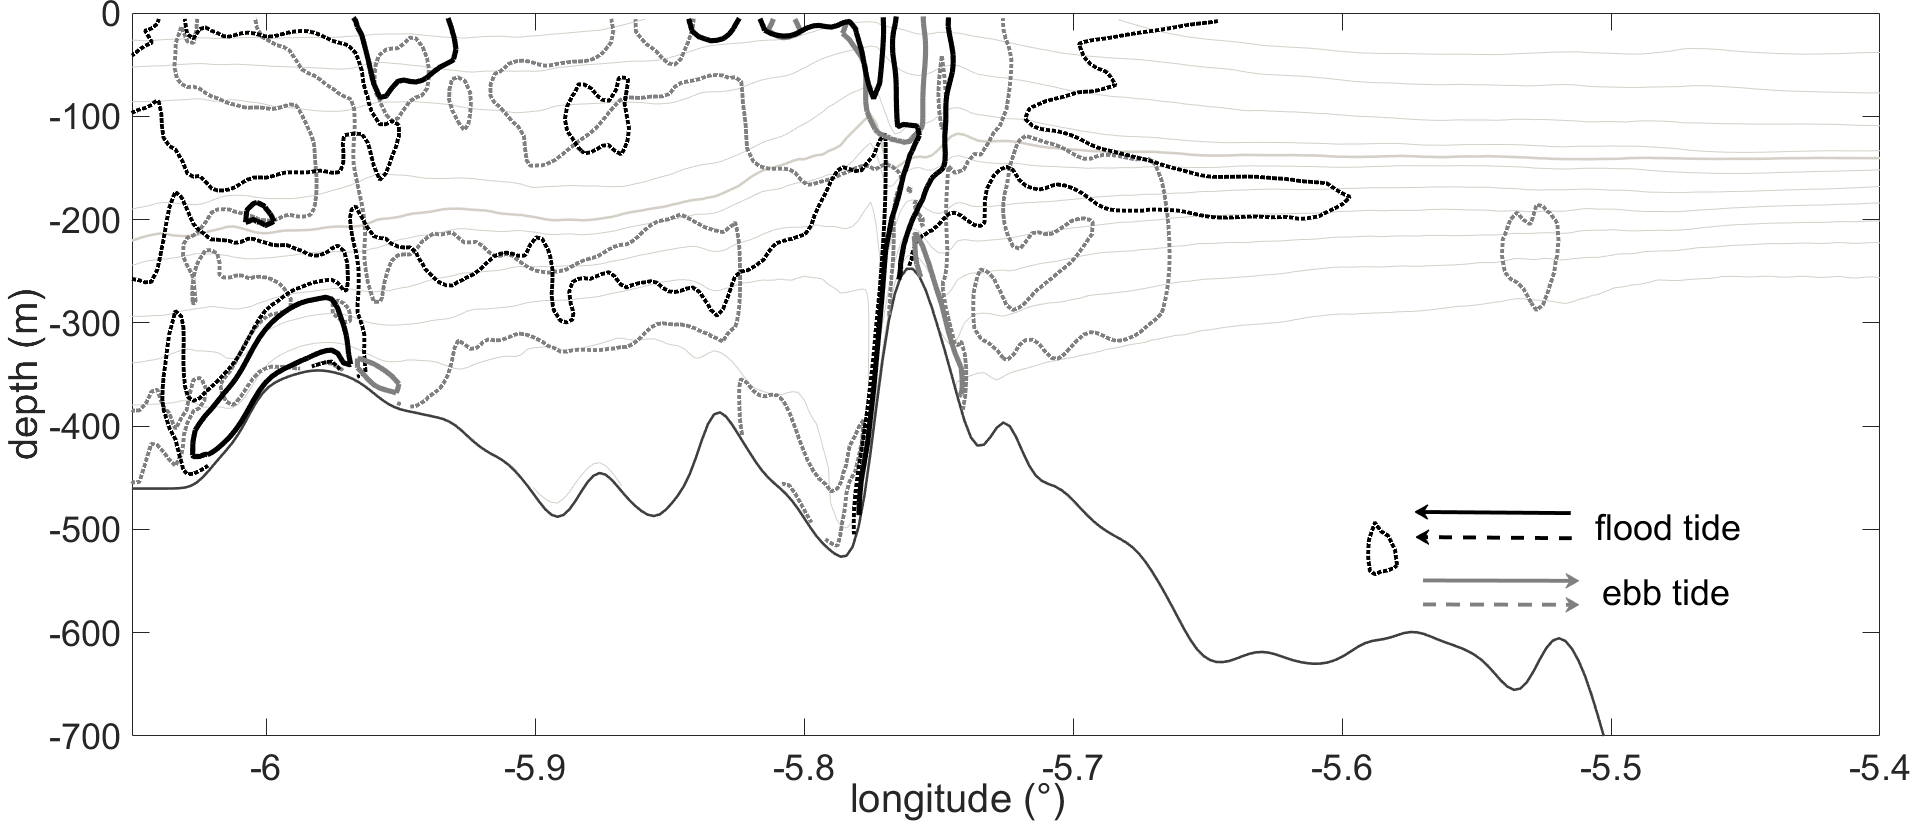
\includegraphics[width=1\textwidth]{./papier2D/Fn_1-2_ref_3T.png}
 \caption{Averaged isopycnal position over 3T (bolded p = -0.7) and region where F > 1 for mode 1 inflow (black) outflow (grey) and for mode 2 inflow (dotted black) outflow (dotted grey) for \textbf{SimRef}. Averages are calculated at maximal inflow and outflow, see figure \ref{hov_ref}.}
 \label{fig_fn_ref}
\end{figure}

A major feature of the dynamics through the Strait of Gibraltar is the so-called "flow criticality" usually characterized with the Froude number ($F$). Several definitions of this non-dimensionnal number can be found in the literature: it can notably be defined for each layer such as in Farmer and Armi (1988) or in Sannino et al (2009). In the present study, the Froude number is simply defined at each grid point as the ratio between the local longitudinal velocity u and the theoretical wave speed $c^*_n$ of the mode-n internal wave, calculated through modal decomposition for each point of the x-axis (see Appendix for details).

Small values of the Froude number ($F < 1$) define a "subcritical" regime, intermediate values ($F \approx 1$) a "critical" regime, and large values ($F>1$) a "supercritical" regime. Hydraulic control appears during the flow transition from subcritical to supercritical and persists when and where large Froude numbers are found. As such, since hydraulic control depends on the current, the existence at a given point of a control can change in time, due in particular to the tidal cycle.

At CS, the tidal current amplitude is of 0.8 m/s. This is sufficient to reverse both the upper-layer mean inflow and lower-layer mean outflow in configurations \textbf{SimAllCor}, \textbf{SimNoCor}, and \textbf{SimRef}. 
%This can be seen in fig.\ \ref{figtransportref} for configuration \textbf{SimRef} where 
The transport (not shown) has a tidal component, with lower (upper) layer transport taking positive (negative) values during flood (ebb) tide. 

In figure %s \ref{fig_fn} and 
 \ref{fig_fn_ref} are plotted the closed contours corresponding to a critical Froude number ($F=1$), inside which the flow is supercritical. The longitudinal velocity fields (u) are taken at maximum outflow (pink and red) at $t = 8.5\ T$ and maximum inflow (cyan and blue) at $t = 9\ T$.
Equivalent maps of supercritical regions can also be plotted for configurations \textbf{SimAllCor} and \textbf{SimNoCor} (not shown).
 The wave speeds are calculated from %the stratification after 70 h for configurations \textbf{SimAllCor} and \textbf{SimNoCor} (figures \ref{fig_fn}.a and b), and from 
 a 3T-time-averaged stratification.% for configuration \textbf{SimRef} (figures \ref{fig_fn_ref}).

First of all, we can see that the supercritical zones for mode 1 are located in the neighborhood of Camarinal and Espartel sills. For all three simulations the control of mode-1 waves occurs on the western slope of CS and ES during the ebb tide. In configuration \textbf{SimNoCor} this extends to the secondary sill of Tanger Bassin. During the ebb tide, the flow is supercritical for mode 1 in both configurations \textbf{SimRef} and \textbf{SimAllCor} on the eastern slope of CS and in \textbf{SimRef} in the neighborhood of ES. Otherwise, the flow is supercritical in the upper layer over CS for all simulations.

Due to the definition of the internal-wave speed (it decreases with mode number n), if supercritical for mode 1, the flow is also supercritical at the same points for mode 2. The regions of supercritical flow for mode 2 can then extend both horizontally and vertically, especially in the pycnocline (see for exemple in figure \ref{fig_fn_ref} during the flood tide).% For example, in configuration \textbf{SimNoCor}, the control spreads on the eastern slope of CS (over bathymetry anomalies).
A supercritical zone for mode 2 can also occur where no mode-1 control is present which is the case in the lower layer at the end of TN during flood tide for the three configurations and during ebb tide for configuration \textbf{SimAllCor}. During the ebb tide this supercriticality of the flow at TN seems to be closely linked to the presence of the mode-1 soliton at the same location. Indeed, the currents induced by mode-1 large amplitude waves can be larger than mode-2 propagation velocities.  

Farmer and Armi (1988) found persistent controls for mode 1 at ES, CS and TN. With their numerical model, Sannino et al. (2009) found only periodical appearances of such controls, except at ES where it is persistent. The discrepancy is probably for a large part due to the method and data used to calculate the composite Froude number. Here, our results indicate a tidal periodicity of mode 1 at both CS and ES but never in TN. The latter is logical since our model does not integrate the convergence of the Strait's lateral boundaries. The lack of perpetual control at ES (which, in the literature, extends to the supercriticality of the Mediterranean outflow away from the strait) may come from the crudely imposed stratification. 
%Mode-2 supercritical regions is more present in the pycnocline (or interface layer). It can also occur at positions where a mode 1 is present in the along-strait (u) velocity field, as is the case at TN (\color{blue} what did you mean by ``structure of the supercritical regions''? I shortened the sentence make sure you agree with the result.\color{black}). 
Comparisons are difficult as Froude number and hydraulic control can be defined in various ways. Furthermore, the "maximal exchange" solution is not clearly defined for models with more than two layers in the Strait. One way to localize these controls could be to follow the motion of the isopycnals.

In figure \ref{CV_ressaut}.a the density field for configuration \textbf{SimRef} is plotted at CS during maximum outflow at t = 8.5 T and through the transition to ebb tide in figures \ref{CV_ressaut}.b to \ref{CV_ressaut}.d.

In figures \ref{CV_ressaut}.a to \ref{CV_ressaut}.c, a depression of the isopycnals can be observed immediatly downstream of CS. This hydraulic jump corresponds to the flow transition from supercritical to subcritical in figure \ref{fig_fn_ref}. In figure \ref{CV_ressaut}.a on the other side of CS the isopycnals are spread in the water column over the secondary crest of CS, looking like a trapped mode-2, but it has disappeared in figure \ref{CV_ressaut}.b.

In figure \ref{CV_ressaut}.c and \ref{CV_ressaut}.d, the tidal current slackens and then its orientation changes. In figure \ref{CV_ressaut}.c a bore crosses the crest of CS and it has then steepened in figure \ref{CV_ressaut}.d when a mode-2 disturbance is crossing CS.% This latter passage is featured in the instantaneous transport of fig.\ \ref{figtransportref}. Indeed, during the very first hours of the flood tide, the upper layer transport has a sudden minimum corresponding to a maximum of the upper layer transport \color{blue} (reformule...) \color{black}: this could correspond to the signature of the mixed waters in mode 2. This may appear more clearly if the transport of the interfacial layer was separated from the transports of the upper and lower layers.\\

Overall, the hydraulic jump that apparently develops west of CS during the flood tide remains during four hours in configuration \textbf{SimRef}. It appears not long after low water. Between figures \ref{CV_ressaut}.a and b the amplitude of the hydraulic jump (displacement of isopycnal $-0.5\ kg.m^{-3}$) increases for example from 100 m to 150 m. It decreases afterwards as a mode-1 wave and then a mode-2 wave are generated and propagate eastward. Smaller jumps occur during flood tide on the estearn side of CS, as well as over ES. \\


\begin{figure}[!h]
\begin{subfigure}{0.5\linewidth}
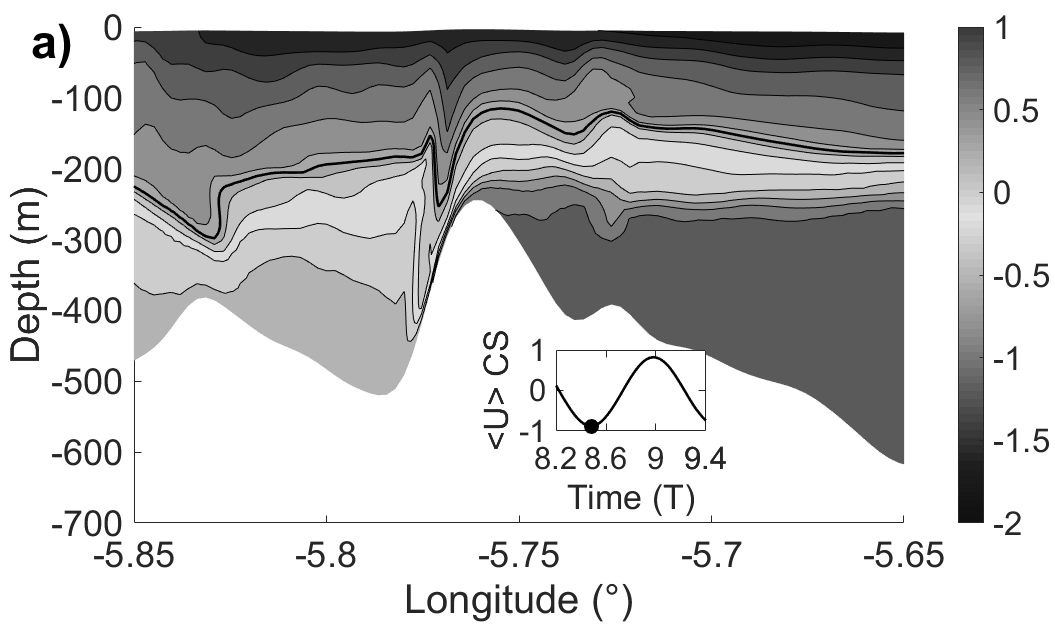
\includegraphics[width=\textwidth]{./papier2D/RW_J4_9h12_ref.png}
\end{subfigure}
 ~
\begin{subfigure}{0.5\linewidth}
  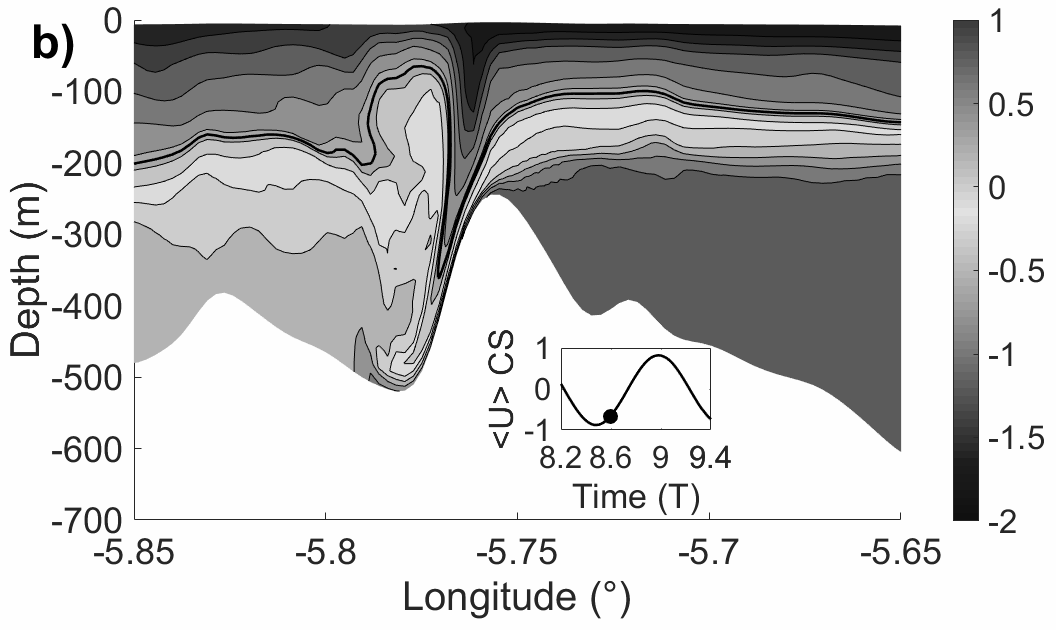
\includegraphics[width=\textwidth]{./papier2D/RW_J4_10h36_ressautebb.png}

\end{subfigure}
 
\begin{subfigure}{0.5\linewidth}
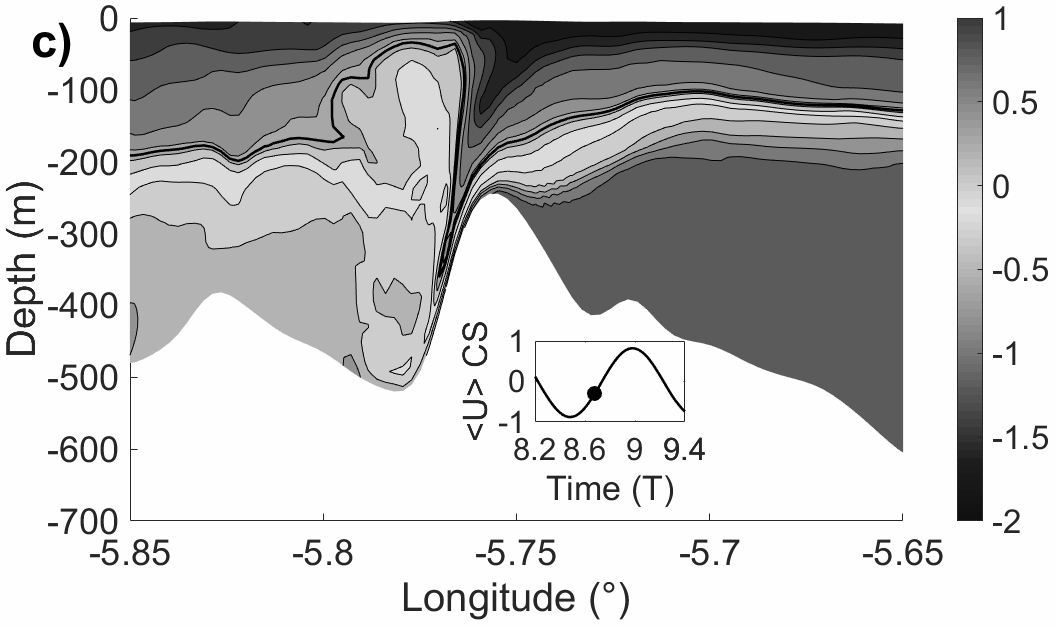
\includegraphics[width=\textwidth]{./papier2D/RW_J4_11h36_deferl.png}

\end{subfigure}
 ~
\begin{subfigure}{0.5\linewidth}
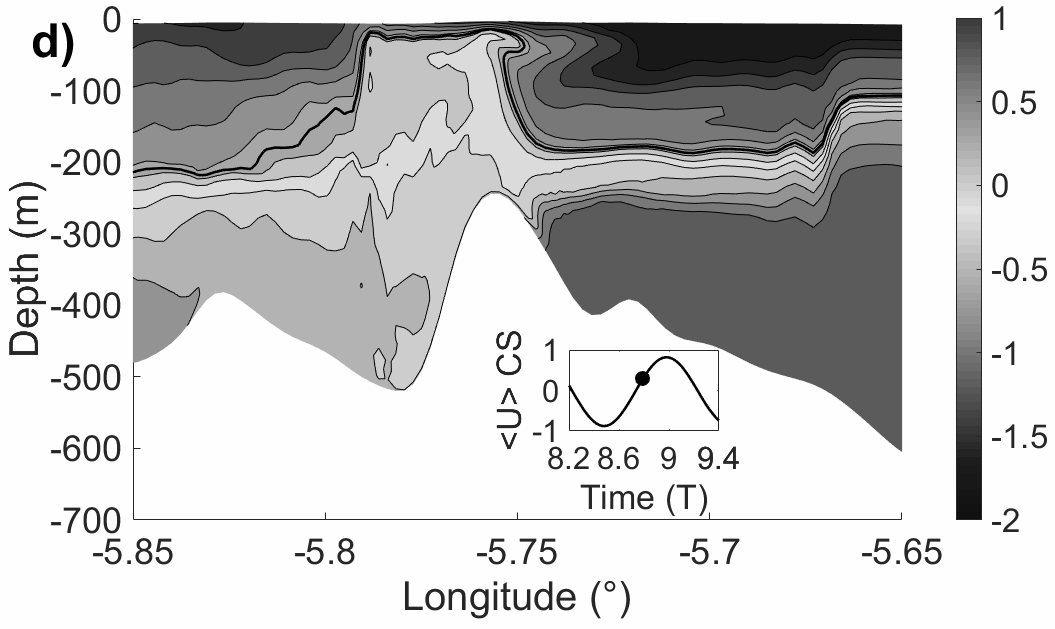
\includegraphics[width=\textwidth]{./papier2D/RW_J4_13h_gen_mod1.png}

\end{subfigure}
 \caption{Density fields of \textbf{SimRef} zoomed over CS, bolded isopycnal: $\rho'\ =-0.5\ kg/m^3$ at t=8.5 T (a), t=8.6 T (b), t=8.7 T (c) and t=8.8 T (d)}
 \label{CV_ressaut}
\end{figure}
 

\paragraph{Internal tide dynamics}
%%%%%%%%%%%%%%
% Figure 5
%%%%%%%%%%%%%%
\begin{figure}[!t]
\centering
\begin{subfigure}{1\linewidth}
\centering
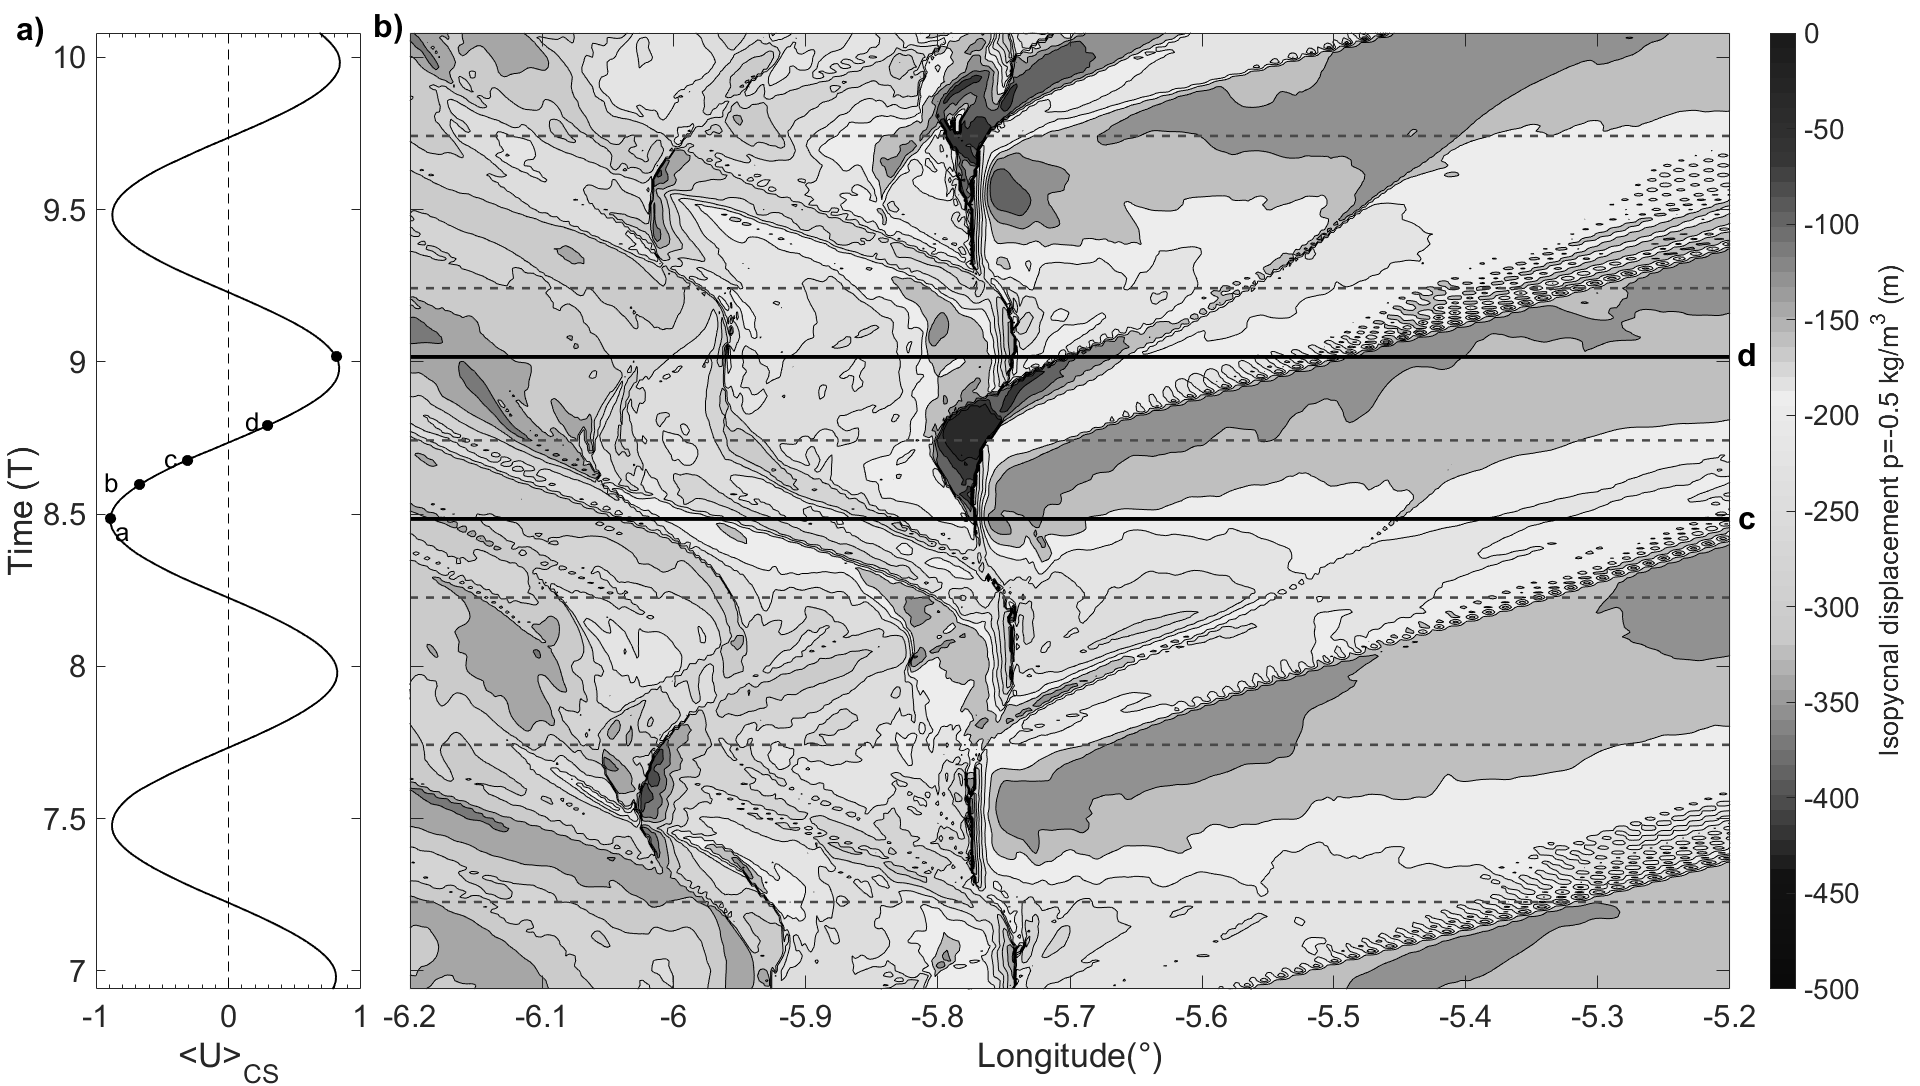
\includegraphics[width=1\linewidth]{./papier2D/hov_ref_-05.png}
\end{subfigure}

\begin{subfigure}{1\linewidth}
   \centering
  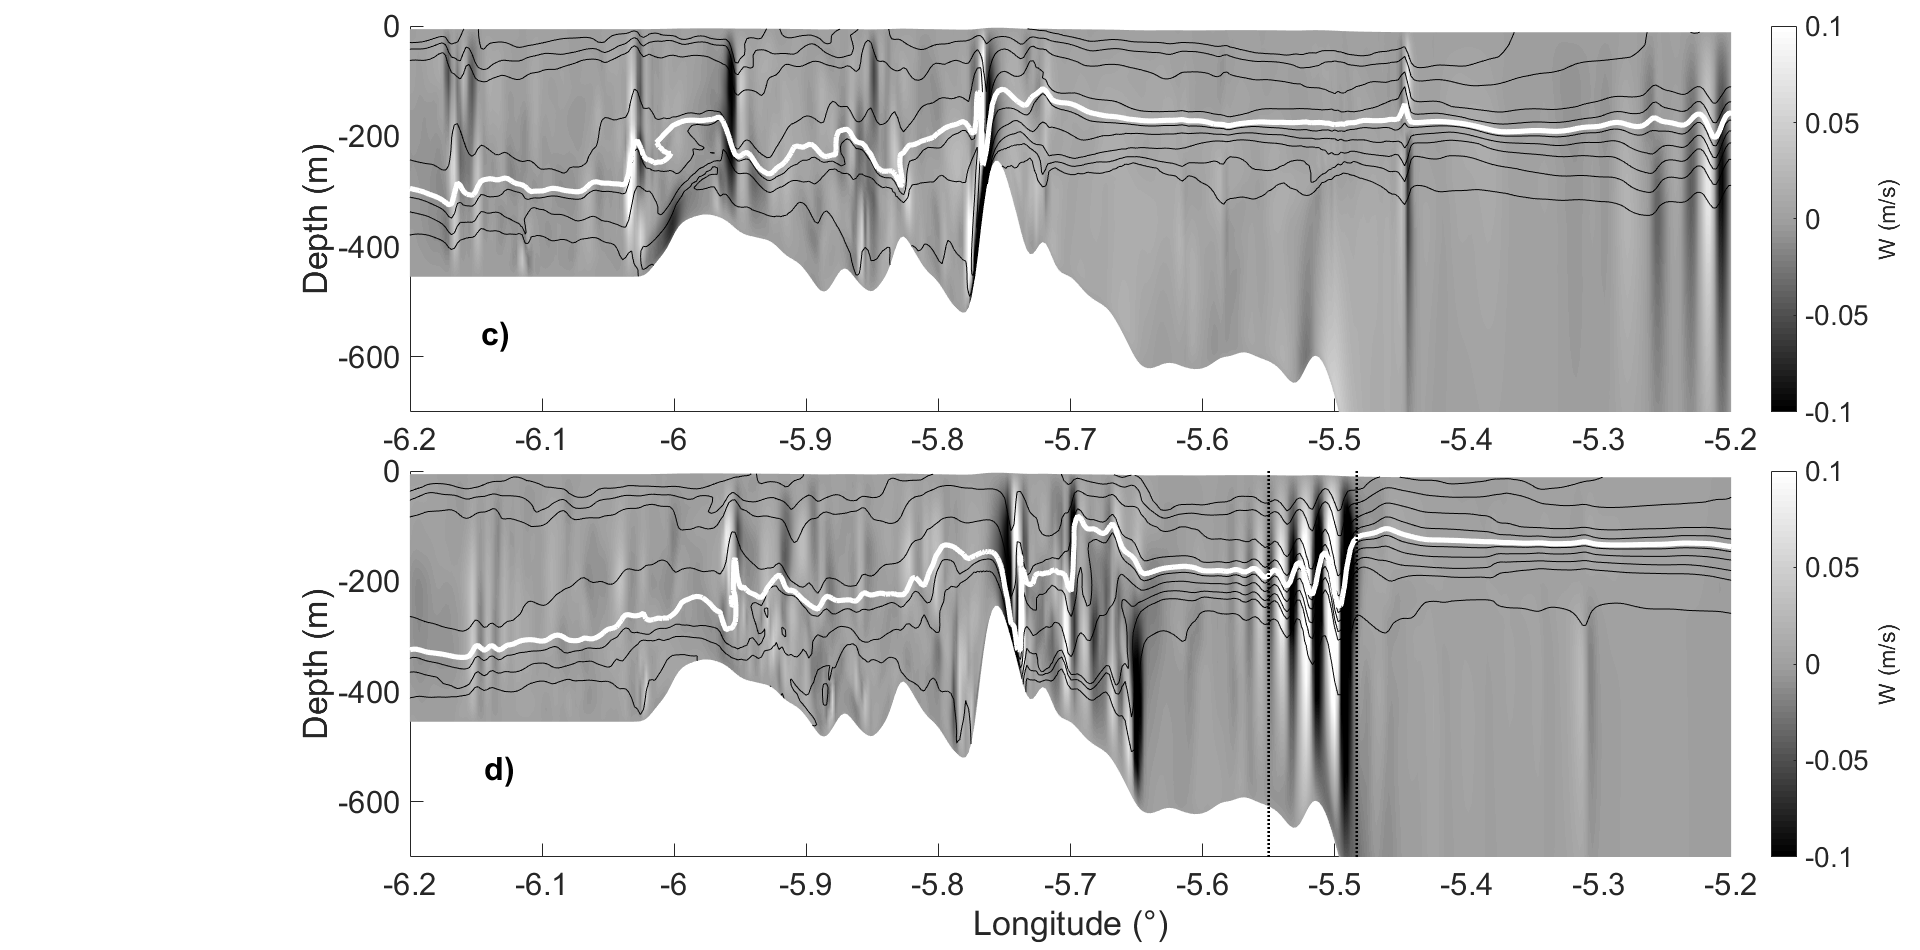
\includegraphics[width=\textwidth]{./papier2D/RW_J4_9h12-15h48.png}
\end{subfigure}
 \caption {(a) vertically averaged current over CS (dots indicate times of plots in figure \ref{CV_ressaut}). (b) Space-time diagram of the vertical displacement of isopycnal $=-0.5 \ kg/m^3$ of \textbf{SimRef}. The dashed lines indicate transition between ebb tide and flood tide, the black lines indicate the times of the two bottom panels. (c) and (d) vertical velocity field and isopycnals at the times indicated in panel (b). In white is the isopycnal $\rho'\ =\ -0.5 \ kg/m^3 $.}
 \label{hov_ref}
\end{figure}

\indent Figure\ \ref{hov_ref}.b is a space-time diagram of the vertical displacement of the isopycnal surface $-0.5\  kg/m^3$ in \textbf{SimRef}. Regions of sharp density gradients can be identified periodically in the region of CS near -5.76°. They correspond to the generation of hydraulic jumps. The propagation of mode-1 and mode-2 large amplitude internal waves can be then followed by the tilt of the isocontours. In this diagram, the slopes correspond to the wave's propagation speed. There are differences from one tidal cycle to the other since, with the mixing, the isopycnal surface gets higher in the pycnocline. In the following, we focus on the tidal cycle t= 8.5 T - 9.5 T (third cycle after the end of the spin-up phase), the corresponding tidal-averaged shear and stratification conditions are shown in figure \ref{fig_current} and figure \ref{fig_fn_ref}.

East of CS a mode-1 wave is generated two hours after the maximum outflow, first as a bore over CS with an amplitude of 100 m and a speed of about 1.3 m/s (as can be seen in figure \ref{CV_ressaut}.d). It continues propagating east in TN as a train of 2 to 3 solitary waves, the first of which has an amplitude of 110 m and a speed of 1.6 m/s. The amplitude of the train of solitons momentarily increases and exceeds 150 m as it propagates over the slope at -5.5° in TN (still with inflowing tidal current).

This ISW train is followed by a mode-2 bore which is generated during the release of the hydraulic jump at high water tide. It goes through CS at a speed of 0.6 m/s and then 0.8 m/s in the shallowest part of TN as a new hydraulic jump remains on the east slope of CS (figure \ref{hov_ref}.d). Its amplitude is then of 100 m. 

With the transition to flood tide, the eastward propagating mode 1 continues its way over the deepest part of the domain. There, the train keeps on being dispersed: when the mode-1 ISWs leave the domain, 7 solitons can be found in the train. The mode-2 bore amplitude decreases and is slowed down by tidal advection: this is for instance the case for a mode-2 bore released during the previous tidal cycle and whose induced velocity signature is still recognizable in the eastern, deepest part of the domain (figure \ref{hov_ref}.c and d).

The signatures of other large amplitude internal waves are visible in the domain west of CS. The western most is a mode-1 wave with an amplitude smaller than the eastward propagating one. It was generated one tidal cycle before by the hydraulic jump in the same way as the train appearing east of Camarinal sill in figure \ref{hov_ref}.

%Figure \ref{figRWna} presents the vertical velocity field and the isopycnals at the same time as figure \ref{hov_ref}.d, but for the configurations \textbf{SimAllCor} and \textbf{SimNoCor}.  
The same figures as in figure \ref{hov_ref} for configurations \textbf{SimNoCor} and \textbf{SimAllCor} can be plotted to follow the forecasted wave dynamics (not shown). In term of speed of the mode-1 wave propagating east of CS, configurations \textbf{SimRef} and \textbf{SimNoCor} are very similar. However, in \textbf{SimNoCor} the amplitude of both mode 1 and mode 2 are smaller and the train of solitons develops only after the wave has descended the slope in eastern TN.

In configuration \textbf{SimAllCor} the speed of the mode 1 wave is of 1 m/s, less than in the other two configurations. The amplitude of the first mode-1 wave is greater and can exceed 200 m. Dispersive effects generate waves to the train in the eastern, deeper part of TN when the wave propagates in the stratified surface layer away from the surface front of Atlantic water.

% \color{red} On peut enlever figure \ref{figRWna}. \color{blue} idem... Je suis d'accord, il faut faire des choix!\color{black}
% %%%%% Figure
% \begin{figure}[!t]
% \centering
% \includegraphics[width=1\linewidth]{comp_15h48_allcor_nocor.png}
% \caption{Field of vertical velocity and isopycnals (white isopycnal $\rho'$=-0.5) in configurations \textbf{SimAllCor} (a) and \textbf{SimNoCor} (b) at the same time as fig.\ref{hov_ref}.d}
% \label{figRWna}
% \end{figure}

In figure \ref{hov_ref}.d %and on both panels of figure \ref{figRWna}
, vertical lines in TN are plotted. They refer to measurments in Farmer and Armi (1988): the lines indicate indeed the position of the two baroclinic modes for each tidal cycle. The right (left) vertical line corresponds to mode 1 (mode 2) three and a half hours after high water, in agreement with the simulations.

In configuration \textbf{SimRef} the distance between the two modes is twice as large (figure \ref{hov_ref}). Mode 1 is well positioned but mode 2 is just entering TN. The same distance between mode 1 and mode 2 can be observed in configuration \textbf{SimNoCor}, whereas the distance between the two modes is closer to observations in configuration \textbf{SimAllCor} though the waves arrive at this positions with a delay. The mode 1 is better positioned in \textbf{SimRef} and \textbf{SimNoCor}.

Based on this measures of wave arrival at various stations, Farmer and Armi (1988) estimated the propagation speed of both mode-1 and mode-2 waves at about 1 to 2.5 m/s for mode 1 and 1 to 1.5 m/s for mode 2. The wave train they observed contained two to three large amplitude waves, the first one having an amplitude of 100 m. 

Other measures in S\'anchez Garrido et al. (2008) estimated a mean propagation speed for the mode-1 waves in TN between 1.2 m/s and 2 m/s with an important diurnal variation.

The mode-1 waves in both the configurations \textbf{SimRef} and \textbf{SimNoCor} have a propagation speed in this range whereas the ones in configuration \textbf{SimAllCor} are too slow and their amplitude is too large.


%%%%%%%%%%%
%\paragraph{Compared dispersion and dissipation with Korteweg-de Vries (KdV) dynamics and satellite images}

%We basically discuss here the contain of Lucie's NumLab to which we can add a comparison with a sequence of Sat images...
%(
\paragraph{Comparison with Korteweg-de Vries (KdV) dynamics}
%)

\begin{figure}[!h]
\centering
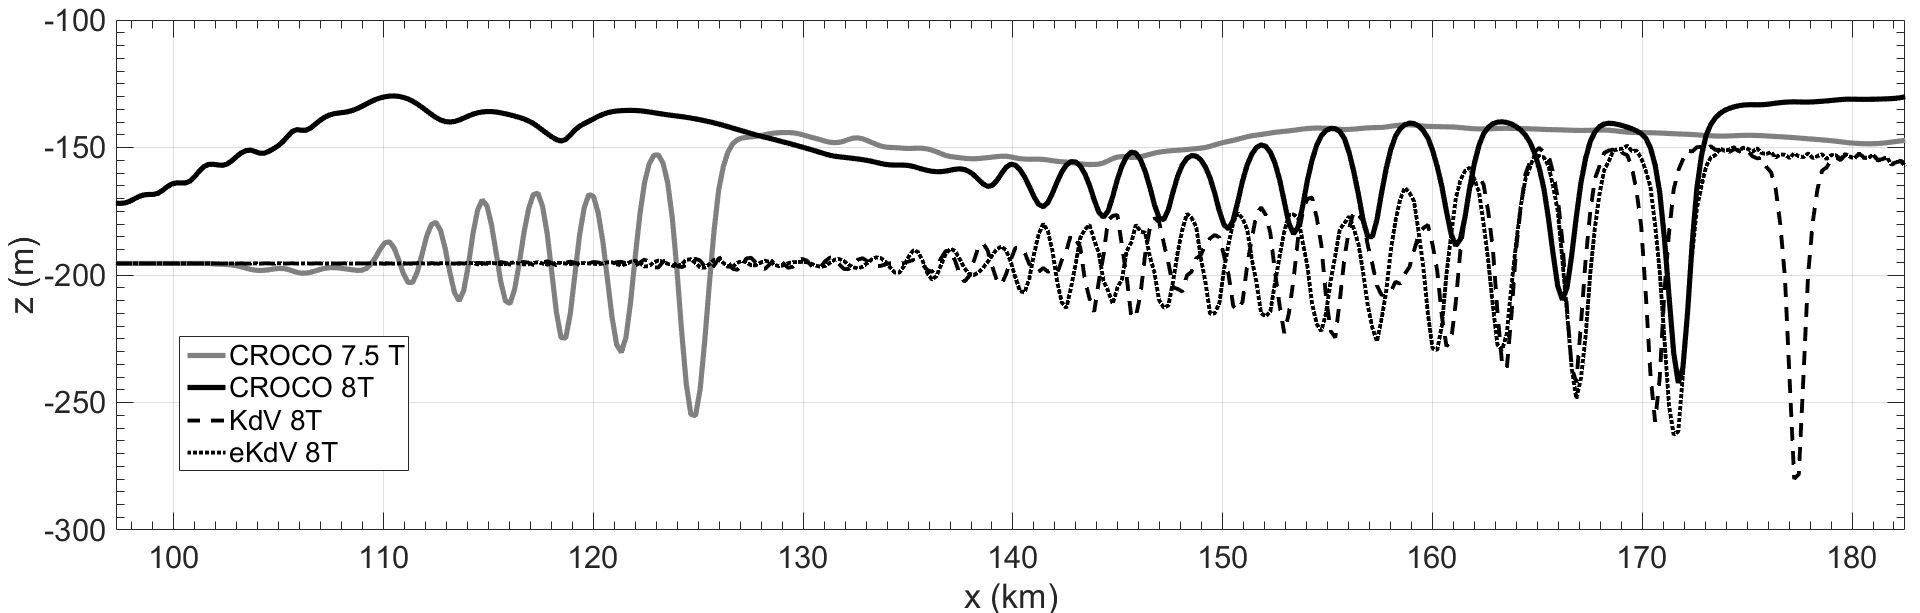
\includegraphics[width=1\linewidth]{./papier2D/exp_kdv_75-8T.png}
\caption{Isopycnal $\rho$'=-0.5 kg/m$^3$ simulated by CROCO-NBQ at t=7.5 T (grey) and t=8 T (black). Evolution of the interface as simulated by KdV (dashed) and eKdV (dotted).}
\label{fig_kdv}
\end{figure}

In previous subsections large amplitude waves propagating over large distance have been compared to available observations. Following many authors (S\'anchez-Garrido et al., 2008, Vlasenko et al., 2009, Sannino et al., 2009b) some of these waves were termed ``ISWs'' for Internal Solitary Waves. We shall now verify if these waves correspond to solutions of the Korteweg-de Vries equation recalled bellow. For these solutions, non-hydrostatic dispersion balances non-linearity. Non-linearity steepens the edge of the wave, whereas non-hydrostatic dispersion is associated to a transfer of energy from large to  small scales, resulting in relatively stable entity called ``solitary'' waves. 

The Korteweg-de Vries (KdV) equation describes the evolution of an infinitely thin interface in a two-layer system with constant bottom topography:
\begin{equation}
\frac{\partial \zeta}{\partial t} 
+c^* \frac{\partial \zeta}{\partial x}
\underbrace{+ \frac{3}{2} \frac{h_1-h_2}{h_1h_2} c^* \zeta \frac{\partial \zeta}{\partial x} }_{A}
\underbrace{+ \frac{1}{6} h_1h_2c^* \frac{\partial ^3 \zeta}{\partial x^3} }_{B}
\underbrace{ - \frac{3}{8}\zeta^2c^*\frac{h_1^2+6h_1h_2+h_2^2}{8(h_1h_2)^2} }_{C}
=0
\label{eq_kdv}
\end{equation}
where $c^*$ is the linear wave speed of small-amplitude internal waves: $c^*=\sqrt{g' h}\ = \ R*f$ and $\zeta$ is the vertical displacement of the interface. $g'$ and $h$ where previously defined in subsection 3.1.

The first two terms on the left hand side of (\ref{eq_kdv}) correspond to a classical propagation equation of a small-amplitude, linear, interfacial wave propagating in the x-direction at a velocity $c^*$. The third term on the left hand side, (A) in (\ref{eq_kdv}), is a first-order approximation (in term of amplitude) of the non-linear advection. The following term (B) is a dispersive term.

The fifth term (C) is a higher-order non-linear term associated to a second order development of advection. This complete equation (\ref{eq_kdv}) will be referred as the "extended KdV (eKdV)", whereas without term (C) it will be simply referred as KdV (Dossmann et al. 2012). 

The large amplitude waves simulated in the previous subsection are now compared to the solutions of the (e)KdV equation to make sure they are ISW. To this aim, we run a new simulation, called \textbf{SimRef+}, with the characteristics given in table \ref{tabsimref} except that (i) the eastern boundary is further east (845 horizontal points, $\rho_0\ =\ 1033.9 \ kg/m^3$) and (ii) the tidal forcing is stopped after only 7.25 periods. The first eastward-propagating train of mode 1 waves generated by the tide at CS in CROCO-NBQ is compared with the propagation given by numerically integrating the (e)KdV equation (\ref{eq_kdv}).

The vertical displacement of isopycnal $\rho'\ =\ -0.5\ kg/m^3$ is extracted at $t_0\ =\ 7.5\ T$ when the mode-1 ISW train is propagating over a region of constant depth H = 890 m west of TN and is represented in figure \ref{fig_kdv}. At that time, the distance between the first and second wave is of 3.3 km, the first wave of the train has an amplitude of 104 m and the train has 6 waves. This isopycnal is chosen as the initial state for the (e)KdV framework. The mode 1 linear propagation speed is computed from this initial state: $c^*\ =\ 1.53\ m/s$.

Figure \ref{fig_kdv} compares the depth of interface obtained at $t\ =\ t_0\ +\ 0.5\ T$ with the KdV and eKdV equations with the position of the $-0.5\ kg/m^3$ isopycnal surface in \textbf{SimRef+}. For the CROCO-NBQ simulation, the distance between the first two waves of the train is 5.5 km with an amplitude of 104 m for the first trough. The train is made of ten waves. It is followed by a disturbance caused by a smaller amplitude internal wave that was generated during the inflow.

In figure \ref{fig_kdv}, the second-order advection term in eKdV adds dissipation. This term slows down the wave and reduces its amplitude. As a result, the speed of the first wave and its amplitude are coherent with the ones simulated in CROCO-NBQ. The distance with the second wave of the train is also closer to CROCO-NBQ in eKdV (4.6 km) than in KdV (6.9 km). In both KdV and eKdV, the train has more waves than simulated by CROCO-NBQ.

The shape and evolution of the large amplitude waves appearing in \textbf{SimRef+} are consequently close to the one predicted by the (e)KdV equation (\ref{eq_kdv}) confirming that (i) this large amplitude wave propagate as ISW and (ii) CROCO-NBQ provided an accurate simulation of ISW in realistic conditions. Both the NH-kernel (for NH dispersion) and the advection schemes (for non-linearity) of the code are concerned.\\


%----------------------------------------------
\paragraph{Comparison with Satellite images}
%\begin{wrapfigure}[16]{r}{0.5\textwidth}
\begin{figure}[!h]
 \centering
 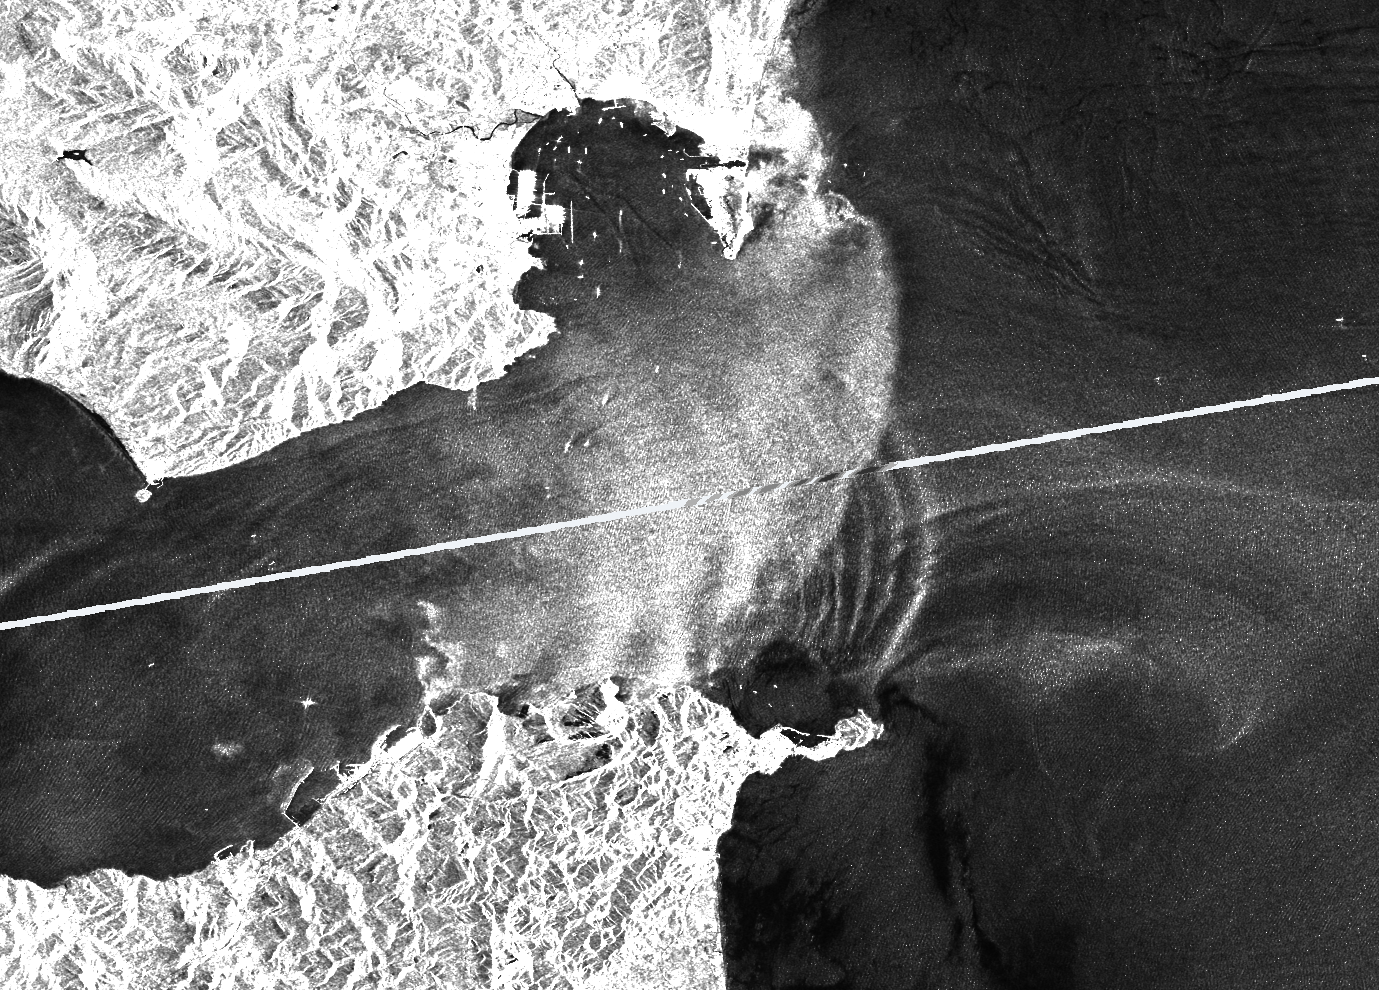
\includegraphics[width=0.45\textwidth]{./papier2D/sat_2dref_20042016_zoom.png}
 \caption{SAR image of Sentinel 1 the 20/04/2016 at 6h27 UTC and absolute value of the slope of $\eta$ in \textbf{SimRef} (in red the slope is non-zero). }
 \label{sat2d}
\end{figure}
%\end{wrapfigure}

Yet another comparison of the ISW propagation can be made with SAR\footnote{SAR: Synthetic Aperture Radar} satellite data (Alpers, 1985). Figure \ref{sat2d} presents an image of the recently launched, high-resolution, Sfentinel 1 SAR that shows a train of mode-1 ISW leaving the strait at a time corresponding to low-water. The absolute value of the gradient of the free-surface elevation ($\vert \partial \eta / \partial x \vert$) is superposed at $t = 7.25\ T$ in simulation \textbf{SimRef}. The wavelength of the first wave in the simulation can for instance be deduced by measuring the distance between the first and third black patch on the transect in figure \ref{sat2d}.\color{black}

In the satellite data, a distance of 1.5 km is measured between the first two waves, of which we can count 6 in total. By comparison, there are also 6 waves in the simulation, but they have a longer wavelength with a distance of 2.6 km between the first two.

The discrepancy in position can be explained by the tidal amplitude which is smaller in the simulation. As a consequence, the solitary waves propagated more slowly (Farmer and Armi, 1988). However, the larger wavelength means that the 2D configuration is too dispersive, maybe in part because there are 3D effects (such as possible interactions with the strait boundaries) which reduce the dispersion and are not taken into account.\\


%%%%%%%%%%%%%%%%%%%%%%%%%%%%%%%%%%%%%%%%%%%%%%%%%%%%%%%%%%%%%%%%%%%%%%%%%%%%%
\subsection{Sensitivity to physical factors}
The so-called \textit{Reference configuration} proposed in the previous subsection is based on several physical and numerical choices as well. We now investigate the impact on the strait's small-scale dynamics of both physical (topography and amplitude of the tides) and numerical (spatial resolution and hydrostatic approximation, next section) parameters. 

%\paragraph{Physical factors}

%%%%%%%%%%%%%%%%%%%%%%%%%%%%%%%%%%%%%%%%%%%%%%%%%%%%%%%%%%%%%%%%%%%%%%%%%%%%%

%----------------------------------------------------------------------------
\paragraph{Topography}
%----------------------------------------------------------------------------
\label{TestPhy}

\begin{figure}[!t]
\centering
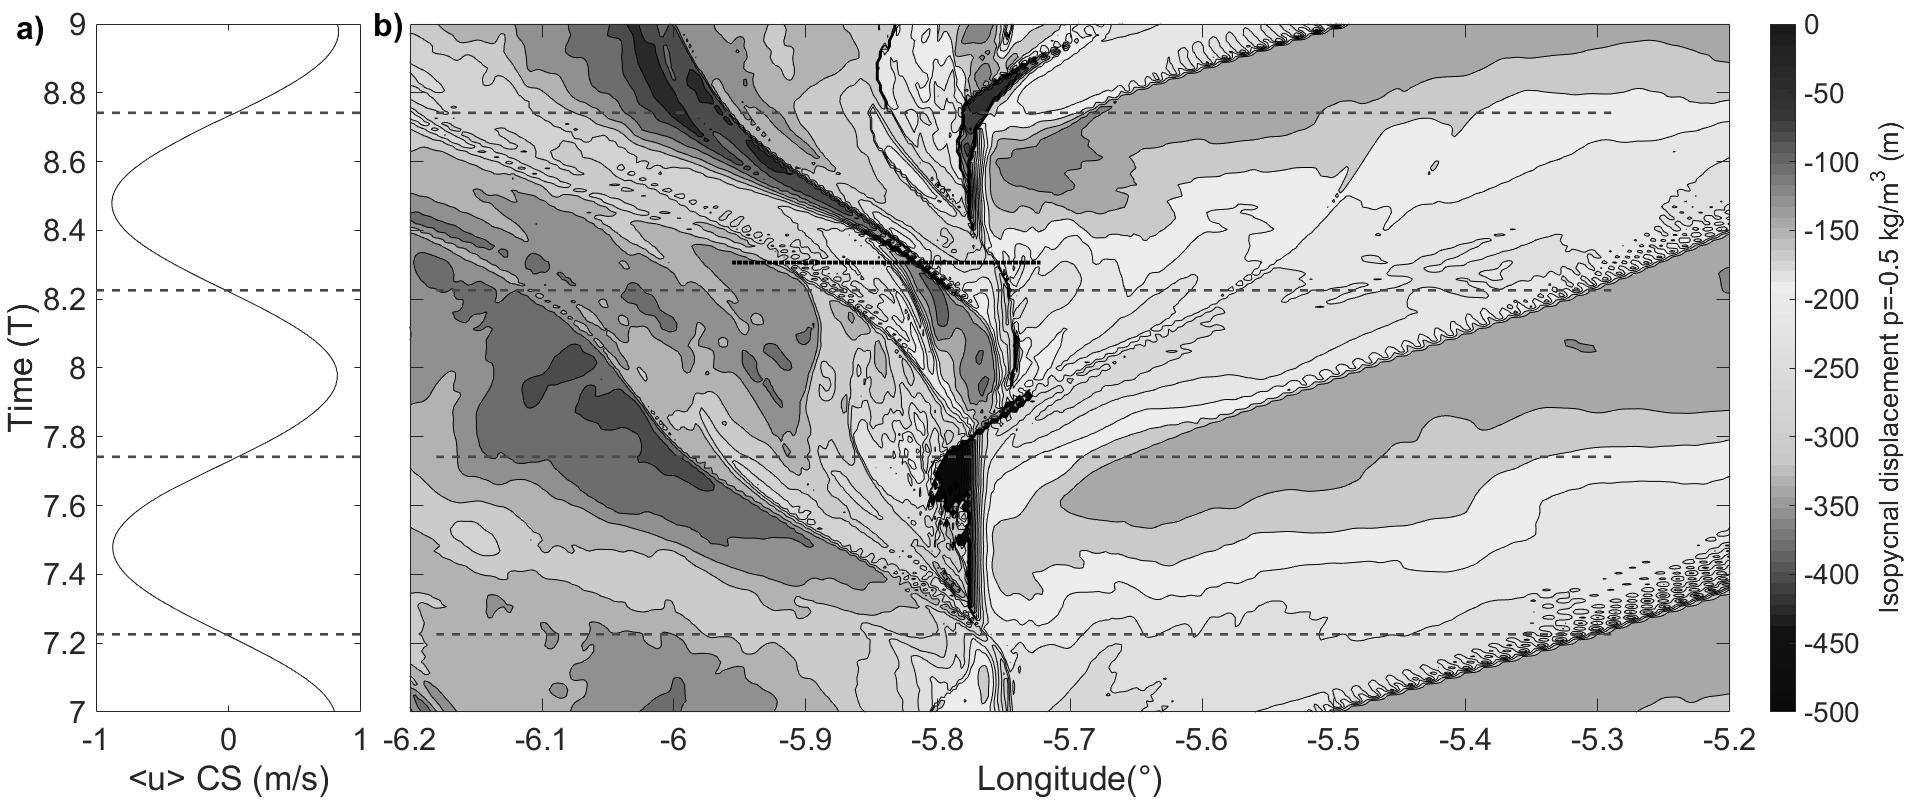
\includegraphics[width=1\linewidth]{./papier2D/hov_p-05_CS.png}
\caption{Same as fig \ref{hov_ref}.a and b for \textbf{SimA}.}
\label{hov_CS}
\end{figure}
\begin{figure}[!h]
\centering
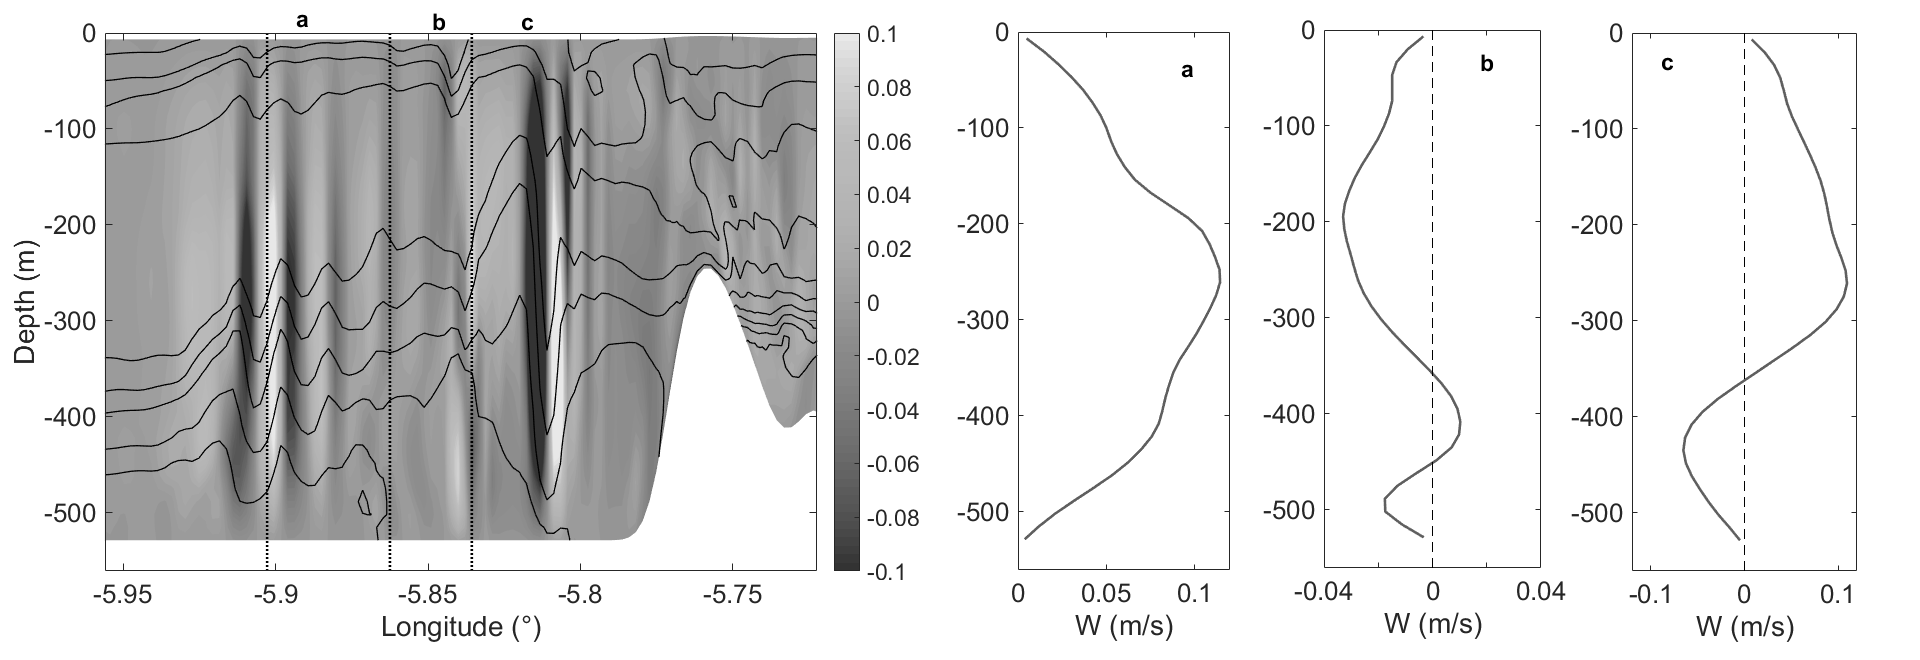
\includegraphics[width=1\linewidth]{./papier2D/w_it515_modes_CS.png}
\caption{Left : field of vertical velocity  and isopycnal contours in \textbf{SimA}. Right: profiles of vertical celerity in the water column.}
\label{figCS_2}
\end{figure}

A first sensitivity simulation, \textbf{SimA}, is run with the same characteristics as the Reference configuration (\textbf{SimRef}, table \ref{tabsimref}), except that all topographic features apart from the bathymetry of CS are smoothed over. East (west) of CS, the resulting depth is constant and is equal to -620 m (-530 m). The reference density is $\rho_0\ =\ 1033.5\ kg/m^3$. The objective is to isolate the effect of CS, especially on the western side of the domain.

Figure \ref{hov_CS} presents the space-time evolution of the vertical displacement of the ispopycnal surface $-0.5\ kg/m^3$. As in subsection 3.1.2 this surface can be used to study the propagation of interfacial internal waves. West of CS, a wave is generated at each tidal cycle shortly before the switch from ebb to flood tide. Figure \ref{figCS_2} depicts a vertical subsection and some profiles of vertical celerity at $t\ =\ 8.3\ T$, showcasing numerous baroclinic waves with characteristic wave structures propagating west of CS : two 50 m-amplitude mode-1 waves (a), a non-negligible mode 2 (c), and small-amplitude mode 3 (b) .

%In the broad scheme, the same dynamics\color{blue} described in subsection ... \color{black}can be observed east of CS in a similar way as in the Reference configuration. 
Firstly, figure \ref{hov_CS} shows that at the beginning of flood tide, mode 1 can also be generated west of CS and escape the domain (as is the case at 7.3 and 8.3 T) whereas higher-order waves are advected back toward the east by the subsequent ebb tide (as can be seen at 7.8 T and 8.8 T). Another mode 1 can also be generated as the jump is established this time west of Camarinal sill (7.9 T, visible in figure \ref{figCS_2}).

Secondly, the amplitude and propagation speeds of the waves traveling west of CS are smaller than the amplitude and propagation speeds of the waves traveling east. For example, the largest mode 1 generated at the end of the ebb tide is slower than the one traveling east, so that it cannot reach the boundary of the simulated domain when the tide switches to ebb tide again. It has then to travel upstream and its speed is reduced from 0.8 m/s to 0.3 m/s. This mode-1 wave is also of smaller amplitude (less than 50 m), and no sign of ISW can be observed.

These waves generated and propagating over a "fake" bathymetry can now be compared to the more realistic dynamics described in \textbf{SimRef} (subsection 3.1.2, figure \ref{hov_ref}). East of CS, the simulated waves are similar, with equivalent speed for modes 1 and 2. West of CS, however, the waves interact with the topography of Tanger Bassin and ES. In particular, the effect of the hydraulic control over ES is evident in figure \ref{hov_ref} as the westward waves cannot propagate during flood tide and interact with the hydraulic jump on the western flank of ES during the ebb tide. 


%----------------------------------------------------------------------------
\paragraph{Amplitude of the tides}
%----------------------------------------------------------------------------

A second sensitivity simulation, \textbf{SimB}, is achieved, identical to \textbf{SimRef} except for the amplitude of the tidal forcing. The forcing tidal-current amplitude at the western boundary is now set to 0.6 m/s, so that its amplitude reaches 1.3 m/s over CS. This corresponds to spring-tide regime in the TPXO-8 database.

Figure \ref{fig_cv_spring}.a and \ref{fig_cv_spring}.b present the fields of relative density for this simulation at $t = 8.5\ T$. The corresponding isopycnals in the Reference configuration \textbf{SimRef} are plotted with dashed lines in figure \ref{fig_cv_spring}.b. The contour of the supercritical (F > 1) region is plotted on figure \ref{fig_cv_spring}.a.

In figure \ref{fig_cv_spring}.a the hydraulic jump can be observed west of CS. This jump is also present on the neap-tide configuration \textbf{SimRef}. Moreover, a mode-1 disturbance is trapped east of the shallowest part of CS. This corresponds to an extension in the water column of the supercritical zone in figure \ref{fig_fn_ref}. It begins to propagate eastward when the tidal currents change direction but the bore crossing CS rapidly catches up to it.

In figure \ref{fig_cv_spring}.b eastward propagating mode-1 and mode-2 waves can be observed. The propagation speed of mode 1 is equivalent to the speed found in \textbf{SimRef} (same stratification) but can be slightly slower or faster depending on the tidal cycle. The amplitude of mode 1 is larger, with the amplitude of the first trough reaching 200 m in \textbf{SimB} versus 100 m in configuration \textbf{SimRef}\color{black}. During the outflow, the slowdown of mode 2 when propagating upstream is yet more pronounced and its propagation is thus slower.

Farmer and Armi (1988) showed that the ISW amplitude increases with the tidal current's amplitude during the spring-tide / neap-tide cycle. Also, two hydraulic jumps have been observed together (S\'anchez-Garrido et al., 2011) with transversal assymetry in the Strait as the second one only appears in the northern part of the Strait during spring tide. Finally, during the lowest amplitude tides, generation of ISW can be inhibited by lee-waves over Camarinal Sill (Bruno et al., 2002). This last two phenomenon cannot be properly evaluated in 2D-configuration. 

\color{black}
\begin{figure}[!h]
  \centering
  \begin{subfigure}{0.45\linewidth}
  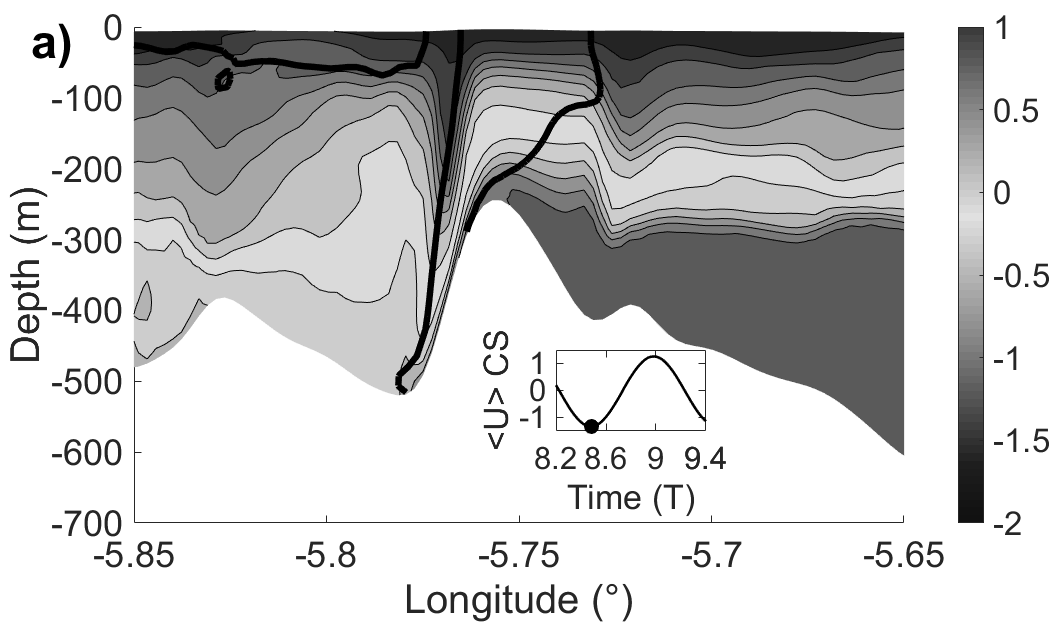
\includegraphics[width=1\textwidth]{./papier2D/RW_j4_9h12_spring.png}
  \end{subfigure}
  ~
    \centering
  \begin{subfigure}{0.45\linewidth}
  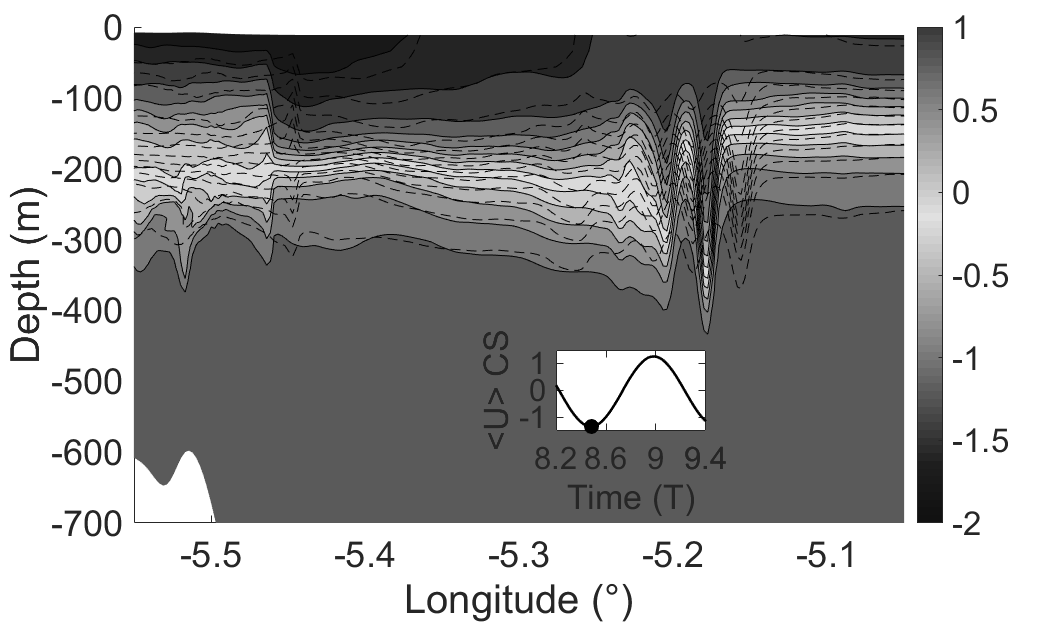
\includegraphics[width=1\textwidth]{./papier2D/CV_train_spring.png}
  \end{subfigure}
  \caption{Relative density contours in \textbf{SimB}.(a) area of F>1 (bolded contour). (b) Relative density contours in \textbf{SimRef}.}
  \label{fig_cv_spring}
\end{figure}


%%%%%%%%%%%%%%%%%%%%%%%%%%%%%%%%%%%%%%%%%%%%%%%%%%%%%%%%%%%%%%%%%%%%%%%%%%%%%
\subsection{Sensitivity to numerical factors}
%%%%%%%%%%%%%%%%%%%%%%%%%%%%%%%%%%%%%%%%%%%%%%%%%%%%%%%%%%%%%%%%%%%%%%%%%%%%%

\paragraph{The spatial resolution}% ($200 \rightarrow 50 m$)}
\label{TestNum}

\begin{figure}[!t]
   
   \centering
  \begin{subfigure}{0.5\linewidth}
  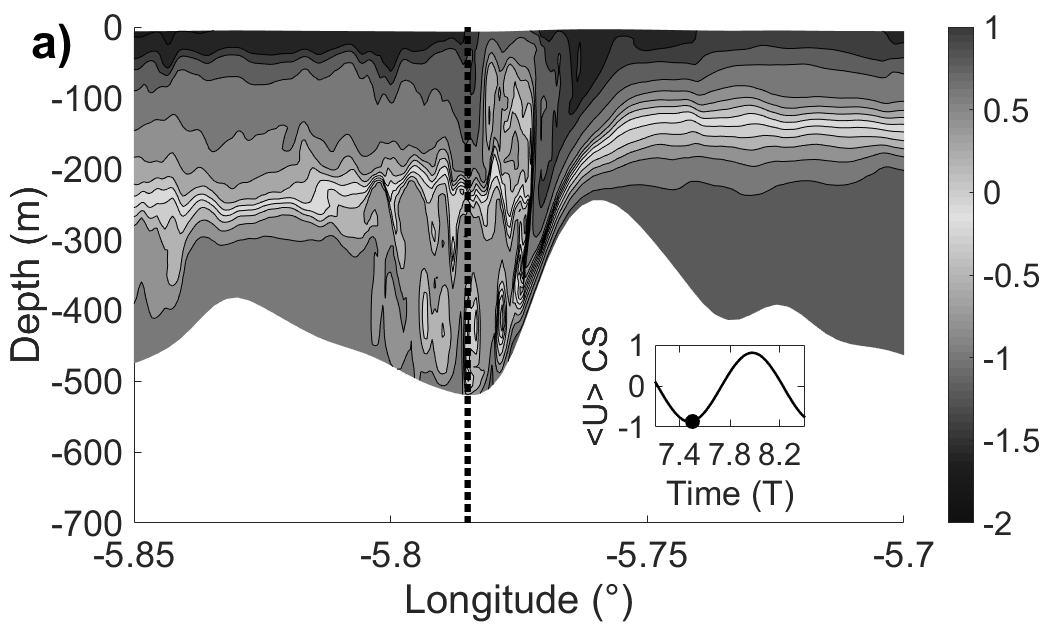
\includegraphics[width=\textwidth]{./papier2D/RW_J3_21h_50mtvd.png}
 % \subcaption{}
  \end{subfigure}
  ~
  \begin{subfigure}{0.5\linewidth}
  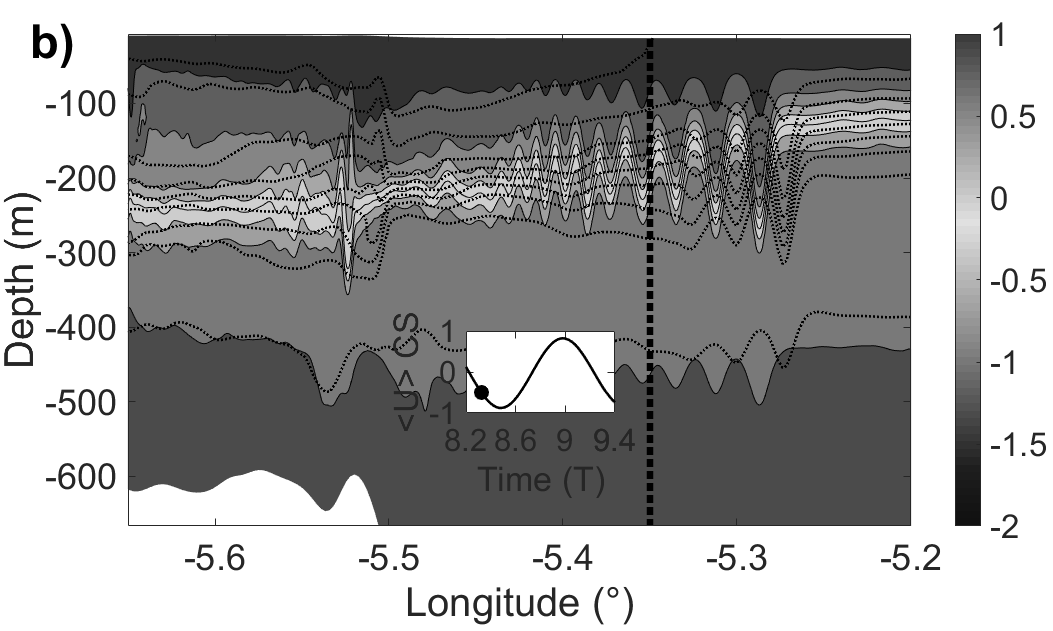
\includegraphics[width=\textwidth]{./papier2D/RW_J4_7h15train_50mtvd.png}
  %  \subcaption{}
  \end{subfigure}
  
  \begin{subfigure}{1\linewidth}
  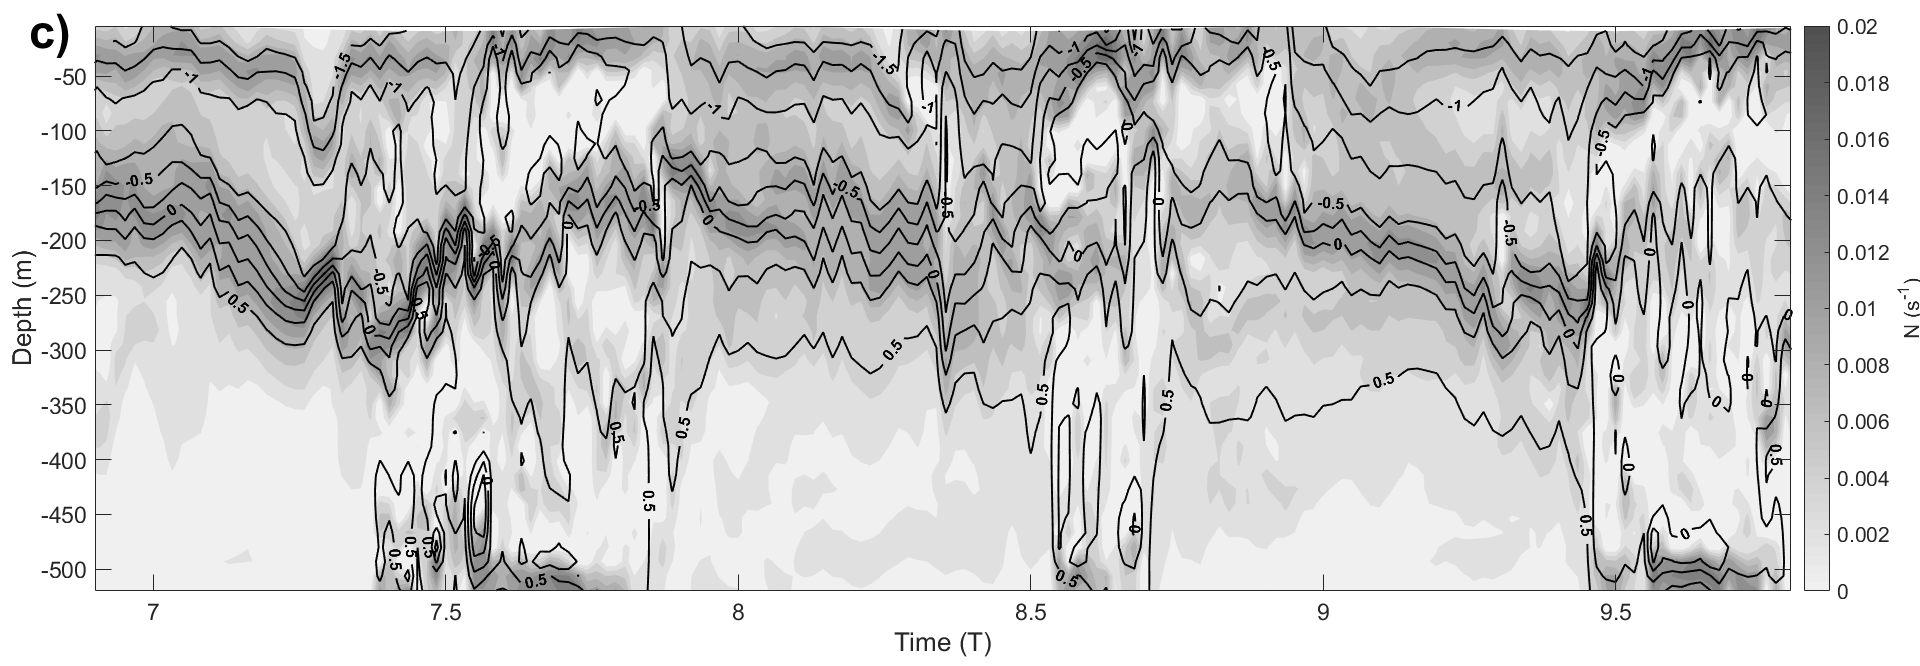
\includegraphics[width=\textwidth]{./papier2D/NrhoTZ_50mNH_5785.png}
  %  \subcaption{}
  \end{subfigure}
     
  \begin{subfigure}{1\linewidth}
  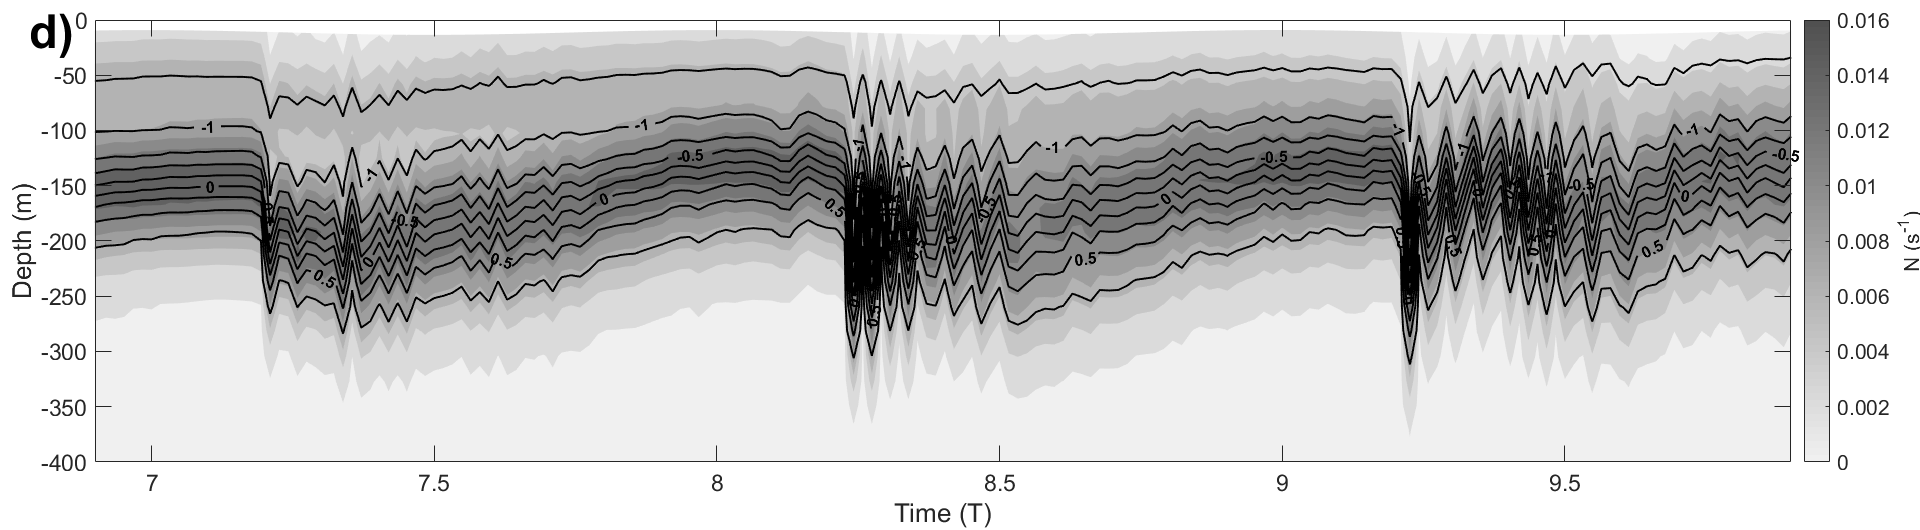
\includegraphics[width=\textwidth]{./papier2D/NrhoTZ_50mNH_535.png}
  %\subcaption{}
  \end{subfigure}
  \caption{(a) and (b) fields of relative density in configuration \textbf{Sim01}. (c) and (d) evolution of the profiles of relative density and $N$ in the water column at the positions of the dashed vertical lines in respectively (a) and (b). (b) dahsed lines are the correponding isopynals for configuration \textbf{SimRef}.}
  \label{fig50mtvd}
\end{figure}

 
% \begin{figure}[!h]
%  \begin{subfigure}{1\linewidth}
%   \includegraphics[width=\textwidth]{NTZrho_ref_5785.png}
%   %\subcaption{}
%   \end{subfigure}
  
%   \begin{subfigure}{1\linewidth}
%   \includegraphics[width=\textwidth]{NTZrho_ref_535.png}
%  % \subcaption{}
%   \end{subfigure}
%   \caption{\textbf{SimRef}}
%   \label{fig220NH}
% \end{figure}
 
A new configuration, \textbf{Sim01}, is investigated. It is identical to \textbf{SimRef} except for the resolution (now $\Delta x = 50\ m$) and time-steps are consequently adapted: $\Delta t_s = 1\ s$ and $\Delta t_f = 1/8\ s$. 

The initial stratification, the (volume) transport through CS and the location of the hydraulic controls (in the neighborhood of CS) are similar (not shown). The initial stratification is also close to the one in configuration \textbf{SimRef}.

Figures \ref{fig50mtvd}.a and \ref{fig50mtvd}.b show isopycnal fields at respectively $t = 7.5\ T$ and $t = 8.3\ T$. Figure \ref{fig50mtvd}.a is a close up on CS and on the hydraulic jump, whereas figure \ref{fig50mtvd}.b focuses on the resulting mode-1 ISW propagating in the deepest part of TN. In figure \ref{fig50mtvd}.b the dashed isocontours indicate the corresponding density field at the same time in the less resolved configuration \textbf{SimRef}. On both figures are featured vertical dashed lines. They indicate the location where the density profile of the water column is extracted to study its evolution in figure \ref{fig50mtvd}.c and \ref{fig50mtvd}.d, as well as the evolution of the Brunt-Väisälä frequency $N$,  given by:
\begin{equation}
N=\sqrt{ - \frac{g}{\rho_0} \frac{\partial \rho}{\partial z}}
\label{eqN}
\end{equation}

%The same evolution of the profile of $N$ at the same positions as for figures \ref{fig50mtvd}.c and \ref{fig50mtvd}.d is plotted in figures \ref{fig220NH}.a and \ref{fig220NH}.b for \textbf{SimRef}. 

A close comparison of figures \ref{CV_ressaut}.a and \ref{fig50mtvd}.a shows that the enhanced resolution allows the explicit modeling of billows west of CS. The comparison of the superimposed fields in \ref{fig50mtvd}.b shows that the mode-1 ISW waves are of comparable amplitude, but the ISW is slower in \textbf{Sim01} with additional waves in the train. Likewise, the mode-2 internal wave is slower in \textbf{Sim01}, and has additional mode-2 waves following it. The pycnocline in figure \ref{fig50mtvd}.d % and \ref{fig220NH}.b 
corresponds to areas where $N$ is large. It is slightly more stratified in \textbf{SimRef} (not shown). It can also be noted that for a same configuration, two consecutive mode-1 trains differ when comparing the number of waves per train.

%In figure \ref{fig220NH}.a, the isopycnal  $\rho' = 0.5\ kg/m^3$ is really deep or even absent in \textbf{SimRef} whereas it is at the bottom of the pycnocline in figure \ref{fig50mtvd}.c (\textbf{Sim01}). 
The lower layer is denser in \textbf{Sim01} than in \textbf{SimRef}. If we look at the other isopycnals, especially in the more stratified zones, there are numerous low-amplitude waves simulated in \textbf{Sim01} that are not present in \textbf{SimRef}, we can also see the signature of the billows as concentric ovals in figure \ref{fig50mtvd}.c. In this region, \textbf{Sim01} is more stratified than \textbf{SimRef}.

The increase in resolution does not change drastically the simulated processes. Indeed most characteristics (transport, speed of propagation, etc) are still of the same magnitude. One more prominent change is the modeling of billows in the hydraulic jump west of CS. An evaluation of the Richardson number (with $Ri =  N^2 / \left({\partial u}/{\partial z}\right)^2$, not shown) shows that $Ri < 1/4$ in the vicinity of the billows. Thus, this billows are potentially associated with Kelvin-Helmholtz instabilities, and linked to the beginning of the turbulent cascade. 
Stratification is deeply affected by the change in resolution, though attributing differences to the implicit dissipation of the numerical scheme or to the now explicitly modeled fine-scale instabilities, requires further sensitivity testing.
 
%%%%%%%%%%%%%%%
\paragraph{The non-hydrostatic algorithm}

\begin{figure}[!t]
  
  \begin{subfigure}{0.5\linewidth}
  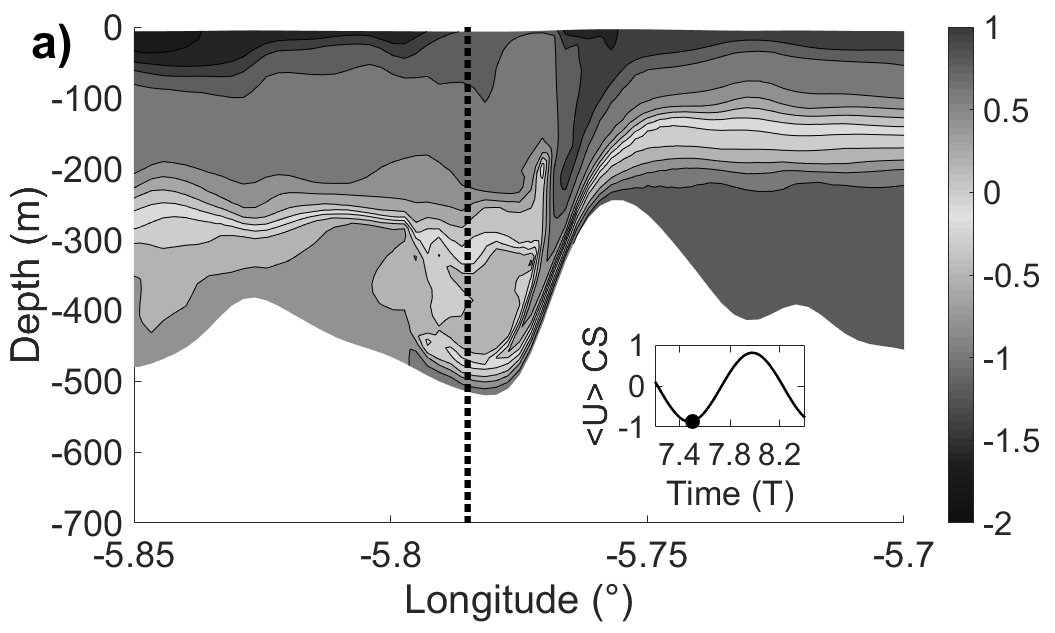
\includegraphics[width=\textwidth]{./papier2D/RW_J3_21_hydro.png}
  %\subcaption{}
  \end{subfigure}
  ~
  \begin{subfigure}{0.5\linewidth}
  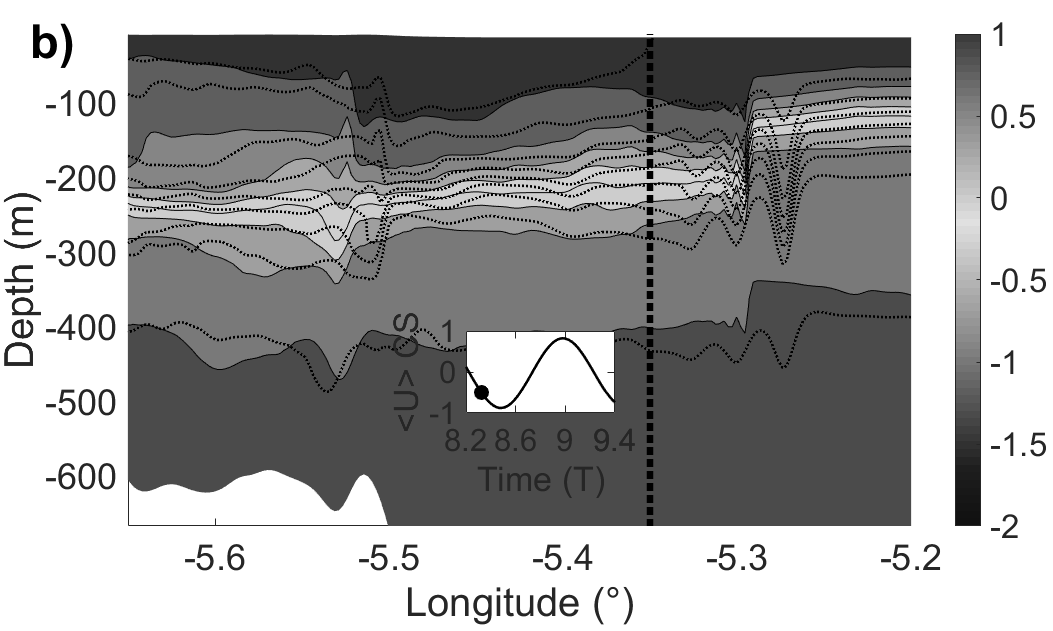
\includegraphics[width=\textwidth]{./papier2D/RW_83T_hydro.png}
  %\subcaption{}
  \end{subfigure}
 
%   \begin{subfigure}{1\linewidth}
%   \includegraphics[width=\textwidth]{Nrho_TZ_hydro_5785.png}
%   %\subcaption{}
%   \end{subfigure}
%   ~
%   \begin{subfigure}{1\linewidth}
%   \includegraphics[width=\textwidth]{Nrho_TZ_hydro_535.png}
%   %\subcaption{}
%   \end{subfigure}
  \caption{Same as figure \ref{fig50mtvd}.a %, b, c and d for configuration \textbf{Sim02}}
  and b for configuration \textbf{Sim02}}
  \label{fig220HNH}
\end{figure}

 Two simulations are now investigated with the hydrostatic version of CROCO. The first one, \textbf{Sim02}, is identical to \textbf{SimRef} (except that it is hydrostatic and its time-steps can be chosen larger: $\Delta t_s = 2\ s$ and $\Delta t_f = 1\ s$). The second one, \textbf{Sim03}, has a spatial resolution of $\Delta x = 50\ m$ and is identical to \textbf{Sim01} with this time two time-steps given by $\Delta t_s = 0.5\ s$ and $\Delta t_f = 0.25\ s$).

 Figure \ref{fig220HNH} %(\ref{figHH}) 
 is the same as figure \ref{fig50mtvd}% (\ref{fig220NH})
 for \textbf{Sim02}. The stratification and transports are equivalent in all simulations.
 
% \begin{figure}[!h]
%  \begin{subfigure}{1\linewidth}
%   \includegraphics[width=\textwidth]{NrhoTZ_50mH_5785.png}
%   %\subcaption{}
%   \end{subfigure}
  
%   \begin{subfigure}{1\linewidth}
%   \includegraphics[width=\textwidth]{NrhoTZ_50mH_535.png}
%  % \subcaption{}
%   \end{subfigure}
%   \caption{50m hydrostatique(\textbf{Sim03})}
%   \label{figHH}
% \end{figure}

 A very first difference, seen for example in figure \ref{fig220HNH}, is the form of the large-amplitude internal waves, that in \textbf{Sim02} is a single wave with a steepened front. This is due to the absence of non-hydrostatic dispersion which, as explained in subsection 3.2.1, induces energy transfers. Hence only non-linear steepening is effective and the waves in the hydrostatic simulations are not ISW. The resulting hydrostatic bore is slightly slower than the first wave of the train in \textbf{SimRef}. The hydraulic jump is similar in both configurations.
 
% Comparing the two hydrostatic configurations, \textbf{Sim02} and \textbf{Sim03}. The effect of this increased resolution are consistent with those in the previous subsection : in the better resolved case the internal bores are slightly slower, west of CS the $0.5\ kg/m^3$ isopycnal line is shallower. The bore in \textbf{Sim03} is steeper (not shown). Both east and west of CS, the 220-m resolved configuration (\textbf{Sim02}) is more stratified (higher values of $N$ are reached in the pycnocline), whereas this was the case only east of Camarinal Sill in the non-hydrostatic configuration.

\begin{figure}[!h]
  
  \begin{subfigure}{0.5\linewidth}
  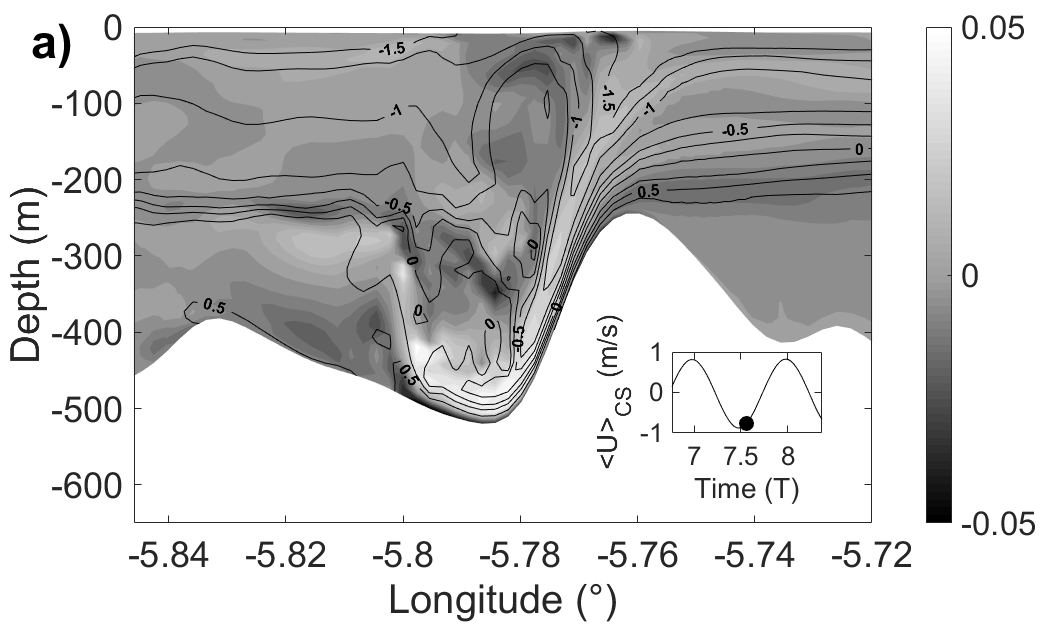
\includegraphics[width=\textwidth]{./papier2D/RV_75T_ref.png}
  %\subcaption{220m NH}
  \end{subfigure}
  ~
  \begin{subfigure}{0.5\linewidth}
  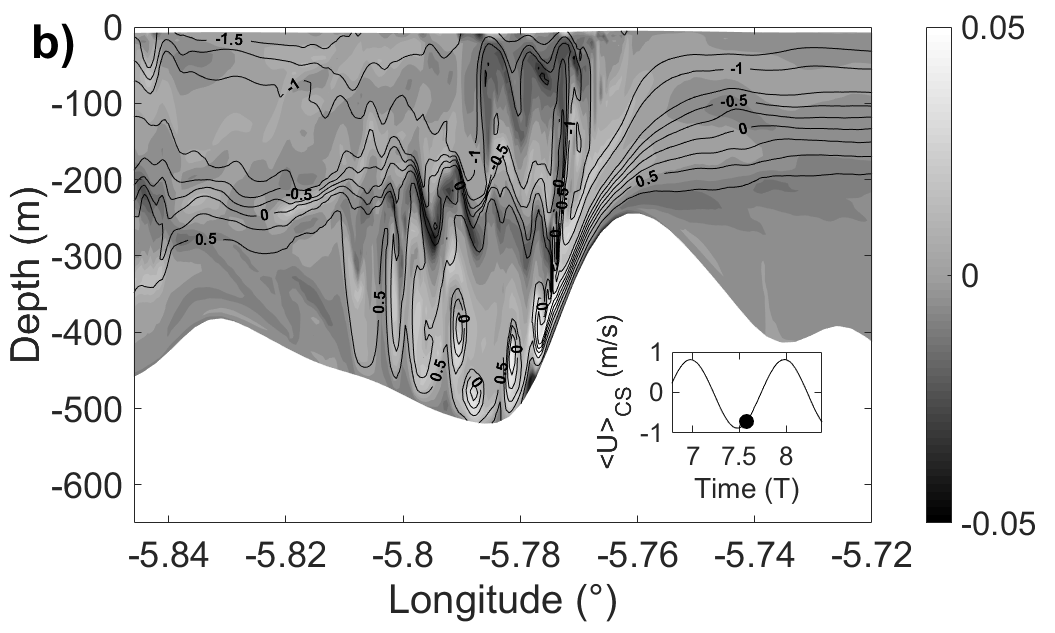
\includegraphics[width=\textwidth]{./papier2D/RV_75T_50m.png}
  %\subcaption{50m NH}
  \end{subfigure}
  
  \begin{subfigure}{0.5\linewidth}
  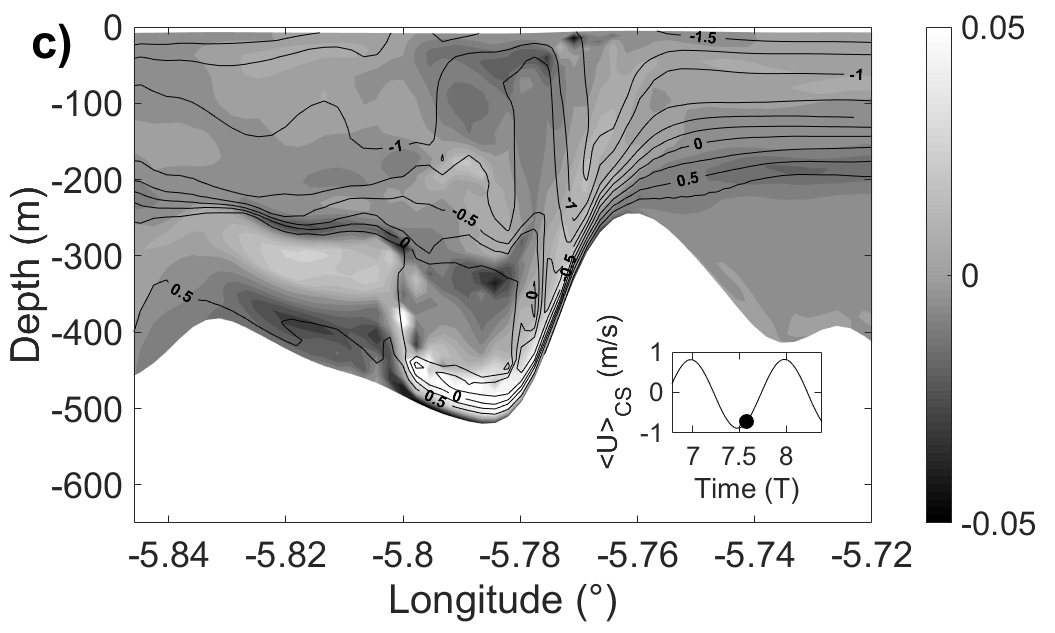
\includegraphics[width=\textwidth]{./papier2D/RV_75T_220mH.png}
  %\subcaption{220m H}
  \end{subfigure}
  ~
  \begin{subfigure}{0.5\linewidth}
  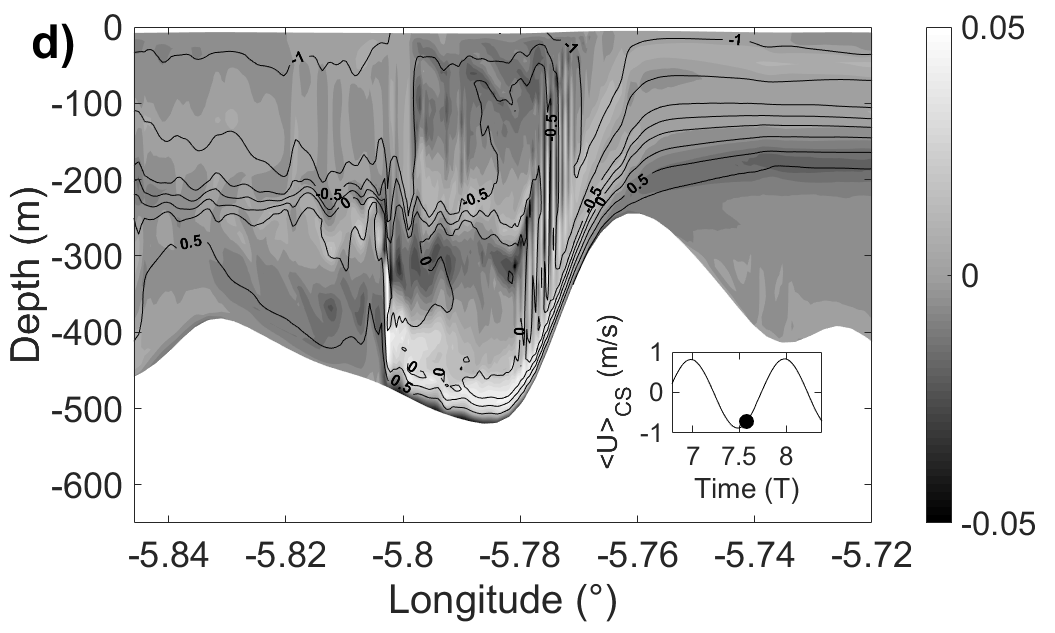
\includegraphics[width=\textwidth]{./papier2D/RV_75T_50mH.png}
  %\subcaption{50m H}
  \end{subfigure}
  \caption{XZ-Vorticity (s$^{-1}$) and isopycnals (kg/m$^3$) for \textbf{SimRef} (a, 220 m non-hydrostatic), \textbf{Sim01} (b, 50 m non-hydrostatic), \textbf{Sim02} (c, 220 m hydrostatic) and \textbf{Sim03} (d, 50 m hydrostatic)}
  \label{figvortCS}
\end{figure}

The same figure as figure \ref{fig220HNH} can be plotted for \textbf{Sim03} (not shown). Comparing the two hydrostatic configurations, \textbf{Sim02} and \textbf{Sim03}. The effect of this increased resolution are consistent with those in the previous subsection : in the better resolved case the internal bores are slightly slower, west of CS the $0.5\ kg/m^3$ isopycnal line is shallower. The wave in \textbf{Sim03} is steeper (not shown). Both east and west of CS, the 220-m resolved configuration (\textbf{Sim02}) is more stratified (higher values of $N$ are reached in the pycnocline), whereas this was the case only east of Camarinal Sill in the non-hydrostatic configuration.

The two 50 m-resolved configurations \textbf{Sim01} (non-hydrostatic) and \textbf{Sim03} (hydrostatic) show different large-amplitude waves and the differences are similar as between the less resolved \textbf{SimRef} and \textbf{Sim02}. However, the effect on stratification seems more visible as the eastern and western parts of CS \textbf{Sim01} are more stratified. A main difference is that the Kelvin-Helmholtz instabilities west of Camarinal Sill, and so the onset of the 2D-turbulent cascade, are only explicitly simulated in \textbf{Sim01}.
The increase in spatial resolution alone is not sufficient to solve the primal instabilities. This requires the implementation of the non-hydrostatic kernel and well-adapted numerical schemes for advection and dissipation (which are indicated in table \ref{tabsimref}).
 
An interesting consequence is that the vorticity balance is well simulated along the x and z-axis in the present vertical subsection. The fields of vorticity in the x-z plane during the outflow at CS are presented in figure \ref{figvortCS} for the four configurations \textbf{SimRef}, \textbf{Sim01}, \textbf{Sim02} and \textbf{Sim03}. In all configurations, positive vorticity structures can be seen associated with the shear of the Mediterranean outflow. In configuration \textbf{SimRef} and the two hydrostatic ones (figures \ref{figvortCS}.a, \ref{figvortCS}.c and \ref{figvortCS}.d), the positive vorticity structure near the bottom is 3-km long and $\approx$ 50-m high, whereas for \textbf{Sim01} (figure \ref{figvortCS}.b) multiple structures of $\approx$ 150-m diameter are visible (the Kelvin-Helmotz instabilities).
 
Mixing is different in all four configurations \textbf{SimRef}, \textbf{Sim01}, \textbf{Sim02} and \textbf{Sim03}, with impact  both of enhanced resolution, and of the combination of enhanced resolution and non-hydrostatic code. However, in less resolved simulation the switch between hydrostatic and non-hydrostatic configuration has a lesser impact.


%%%%%%%%%%%%%%%%%%%%%%%%%%%%%%%%%%%%%%%%%%%%%%%%%%%%%%%%%%%%%%%%
%%%%%%%%%%%%%%%%%%%%%%%%%%%%%%%%%%%%%%%%%%%%%%%%%%%%%%%%%%%%%%%%
%    Rapport intermédiaire de Lucie
%%%%%%%%%%%%%%%%%%%%%%%%%%%%%%%%%%%%%%%%%%%%%%%%%%%%%%%%%%%%%%%%
%%%%%%%%%%%%%%%%%%%%%%%%%%%%%%%%%%%%%%%%%%%%%%%%%%%%%%%%%%%%%%%%

\paragraph{Sensibilité aux schémas d'advection}

\noindent \textit{Cette sous-section, en français est basée sur le rapport intermédiaire $T_0 + 12$ mois écrit par Lucie Bordois, post-doctorante au laboratoire d'Aérologie.}\\

Afin d'évaluer l'impact des schémas d'advection dans la maquette \textbf{SimRef}, une première simulation de référence est réalisée à partir d'un schéma d’advection verticale \textit{« Splines»} (respectivement \textit{« Akima »)} pour la quantité de mouvement (respectivement les traceurs). Ces schémas sont classiquement utilisés dans les maquettes CROCO en version hydrostatique pour des simulations régionales ou côtières.\\
La section verticale 2D (Figure \ref{Fig_TVD1}) montre des oscillations sur les champs de traceurs et de vitesses dans les zones de forts cisaillements verticaux (particulièrement visibles au-dessus de CS durant la phase d’initialisation \textit{« lock-exchange »}. 

%%%%%%%%%%%%%%%%%%%% Figure/Image No: 1 starts here %%%%%%%%%%%%%%%%%%%%

\begin{figure}[!h]
	\begin{Center}
		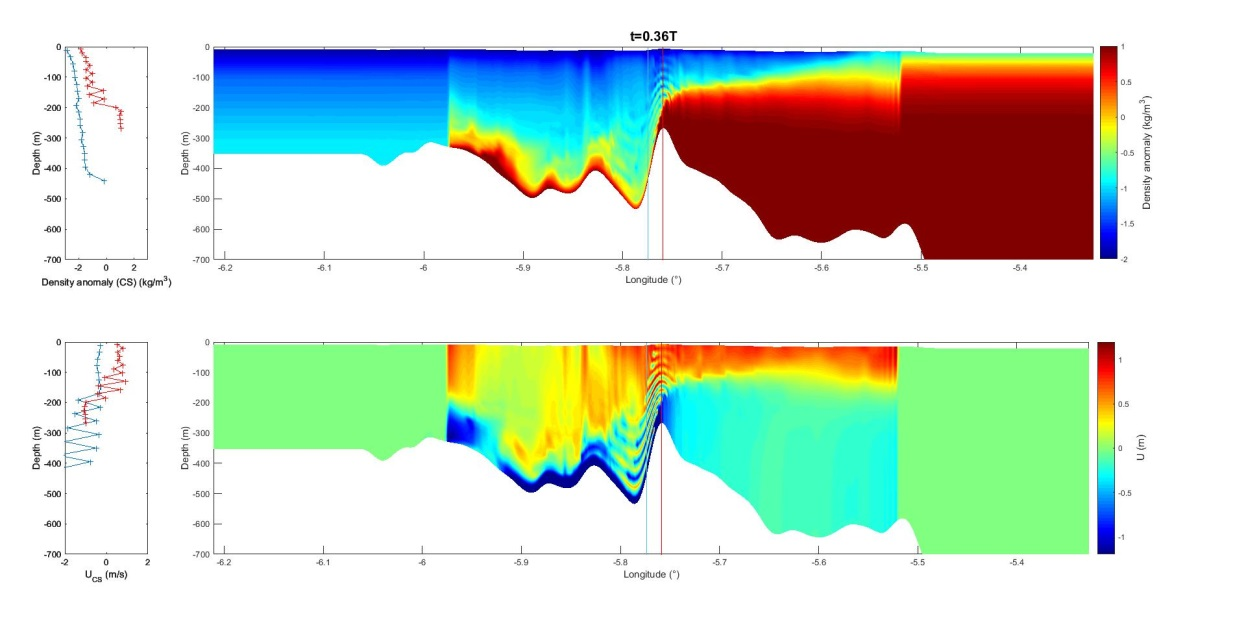
\includegraphics[width=5.66in,height=2.83in]{./media/TVD1.jpeg}
		\caption{ : Section verticale du champ de vitesse horizontale (doite-bas) et du champ d’anomalie de densité (droite-haut) à t=0.36 T (avec T la période de M2) durant la phase de spin-up (initialisation \textit{« lock-exchange »}) dans 2D. (Panneaux de gauche) Profil vertical situé au-dessus de Camarinal Sill (localisé par les lignes rouge et bleue sur les panneaux de droite).}
		\label{Fig_TVD1}
		%\label{fig:_Section_verticale_du_champ_de_vitesse_horizontale_doitebas_et_du_champ_danomalie_de_densit_droitehaut__t036T_T_reprsente_la_priode_de_M2_durant_la_phase_de_spinup_initialisation_Lockexchange_dans_2D_Panneaux_de_gauche_Profil_vertical_situ_audessus_de_Camarinal_Sill_localis_par_les_lignes_rouge_et_bleue_sur_les_panneaux_de_droite}
	\end{Center}
\end{figure}
%%%%%%%%%%%%%%%%%%%% Figure/Image No: 1 Ends here %%%%%%%%%%%%%%%%%%%%

Nous avons donc cherché à évaluer l'impact de différents schémas numériques d’advection et de dissipation turbulente sur ces instabilités numériques. 

\noindent La Figure (\ref{Fig_TVD2} – haut) montre qu'en version 2D-verticale, l’utilisation d’un schéma d’advection de type WENO d’ordre 5 sur la verticale pour les traceurs permet de supprimer l’apparition d’instabilités numériques sur les champs de traceurs. Cependant, les instabilités numériques persistent dans ce cas sur les champs de vitesse (Figure \ref{Fig_TVD2} – bas). Ce résultat montre la nécessité pour la communauté CROCO de disposer de schémas d’advection verticale monotone (type TVD) ou quasi-monotone (type WENO) pour la quantité de mouvement (U, V en hydrostatique et W en version non-hydrostatique). 

%%%%%%%%%%%%%%%%%%%% Figure/Image No: 2 starts here %%%%%%%%%%%%%%%%%%%%
\begin{figure}[!h]
	\begin{Center}
		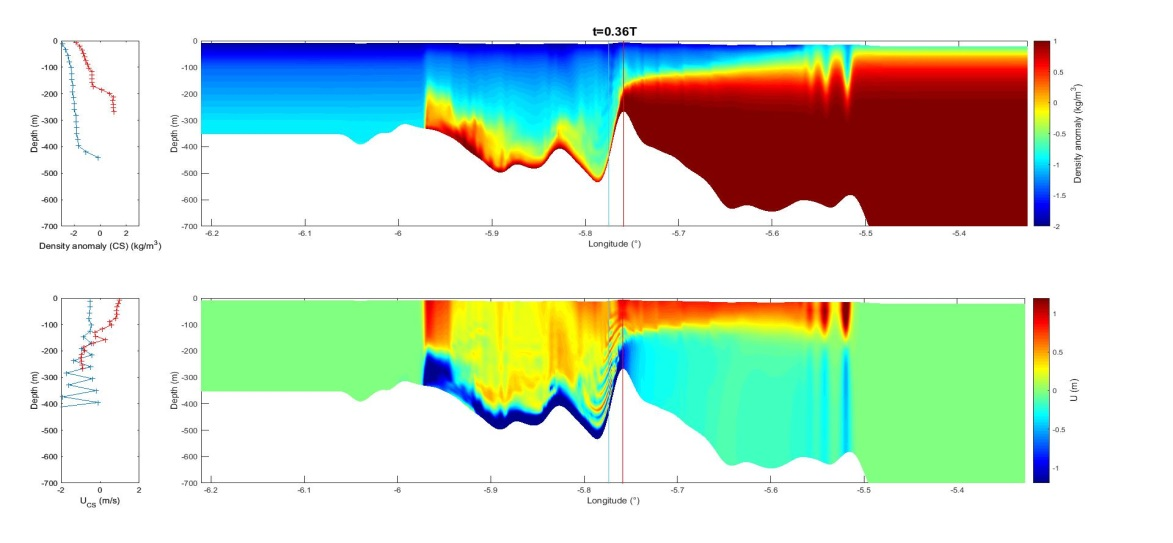
\includegraphics[width=4.98in,height=2.35in]{./media/TVD2.jpeg}
		\caption{ : Section verticale du champ de vitesse horizontale (doite-bas) et du champ d’anomalie de densité (droite-haut) à t=0.36 T durant la phase de spin-up (initialisation « Lock-Exchange ») dans 2DTS-WENO5. (Panneaux de gauche) Profil vertical situé\  au-dessus de Camarinal Sill (localisé par les lignes rouge et bleue sur les panneaux de droite).}
		\label{Fig_TVD2}
		%\label{fig:_Section_verticale_du_champ_de_vitesse_horizontale_doitebas_et_du_champ_danomalie_de_densit_droitehaut__t036T_durant_la_phase_de_spinup_initialisation_LockExchange_dans_2DTSWENO5_Panneaux_de_gauche_Profil_vertical_situ__audessus_de_Camarinal_Sill_localis_par_les_lignes_rouge_et_bleue_sur_les_panneaux_de_droite}
	\end{Center}
\end{figure}

%%%%%%%%%%%%%%%%%%%% Figure/Image No: 2 Ends here %%%%%%%%%%%%%%%%%%%%
\noindent Des schémas d’advection TVD ont été codés par l'équipe de développement CROCO et ont ainsi été testés et comparés dans le cadre du présent contrat. La Figure \ref{Fig_TVD3} (bas) présente un premier résultat montrant la disparition des oscillations lorsqu’un tel schéma est utilisé pour l’advection verticale des composantes horizontales de la quantité de mouvement. La contre-partie anticipable est une augmentation locale de la dissipation liée à l'utilisation du schéma TVD.

%%%%%%%%%%%%%%%%%%%% Figure/Image No: 3 starts here %%%%%%%%%%%%%%%%%%%%

\begin{figure}[!h]
	\begin{Center}
		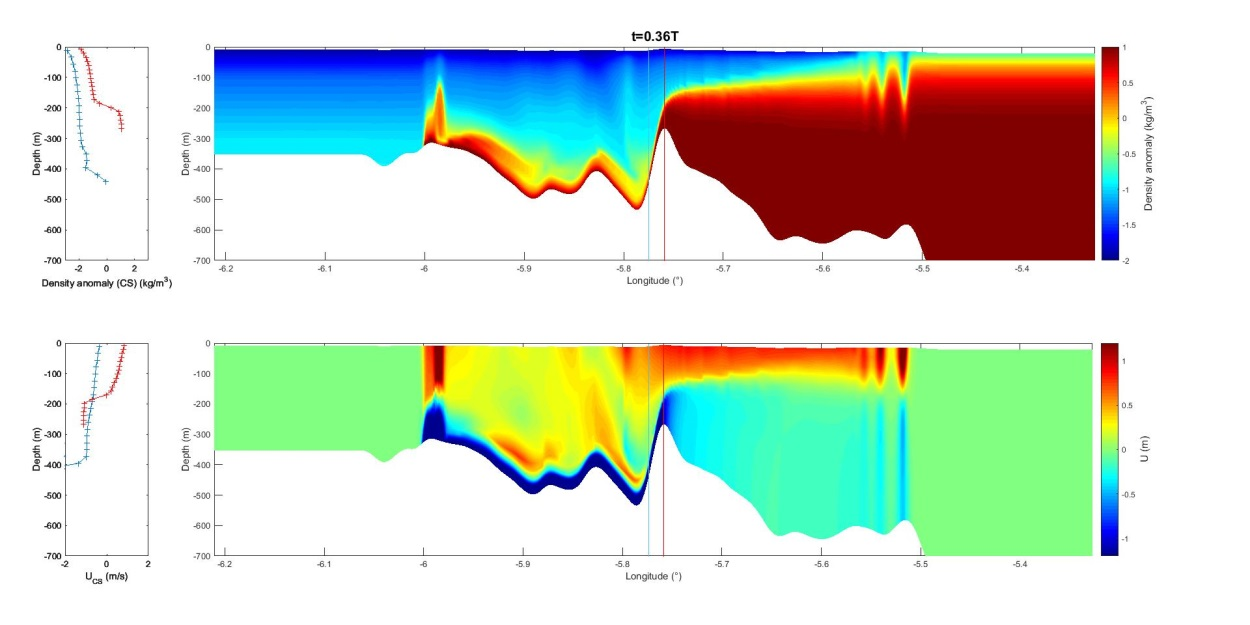
\includegraphics[width=5.68in,height=2.84in]{./media/TVD3.jpeg}
		\caption{: Section verticale du champ de vitesse horizontale (doite-bas) et du champ d’anomalie de densité (droite-haut) à t=0.36 T durant la phase de spin-up (initialisation « Lock-exchange ») dans 2DTS-WENO5,UV-TVD. (Panneaux de gauche) Profil vertical situé au dessus de Camarinal Sill (localisé par les lignes rouge et bleue sur les panneaux de droite).}
		\label{Fig_TVD3}
		%\label{fig:_Section_verticale_du_champ_de_vitesse_horizontale_doitebas_et_du_champ_danomalie_de_densit_droitehaut__t036T_durant_la_phase_de_spinup_initialisation_Lockexchange_dans_2DTSWENO5UVTVD_Panneaux_de_gauche_Profil_vertical_situ_au_dessus_de_Camarinal_Sill_localis_par_les_lignes_rouge_et_bleue_sur_les_panneaux_de_droite}
	\end{Center}
\end{figure}
%%%%%%%%%%%%%%%%%%%% Figure/Image No: 3 Ends here %%%%%%%%%%%%%%%%%%%%

\noindent Les premiers résultats obtenus avec les schémas d’advection de type TVD et WENO confirment un certain nombre de choix numériques assez fondamentaux de la communauté CROCO concernant l’utilisation de schémas numériques « monotones » ou « quasi-monotones ». Les tests de sensibilité réalisés dans le cadre de la présente étude ont de plus montré qu’il était possible de supprimer les oscillations numériques obtenus avec des schémas numériques non monotones plus classiques mais en ayant recours à une dissipation numérique jugée trop importante (coefficient de mélange vertical > 0.001 m²/s $\&$  coefficient de viscosité $ \geq $ 0.1 m²/s) et en tout cas incompatible avec la simulation des trains de solitons observés en aval du détroit (dissipation numérique des trains d’ondes : sous-estimation de l’amplitude des solitons et de leur zone de propagation). Nous avons choisi de ne pas privilégier, dans un premier temps tout au moins, l’implémentation ou l’évaluation de techniques plus sophistiquées pour la modélisation des processus sous-maille et la modélisation des fronts, nous orientant vers des schémas numériques monotones d’advection jugés plus « physiques » et offrant de meilleurs résultats numériques. Ces schémas monotones ne nécessitant pas de schémas de dissipation turbulence numérique additionnels permettent la réalisation de simulation à haute résolution dites MILES pour \textit{(pour Monotone Implicit Large Eddy Simulation)}.\\

\noindent Suite à l’observation dans la simulation 2DV d’oscillations numériques dans les zones de forts cisaillements de vitesse, des schémas d’advection TVD pour l’advection verticale et horizontale des composantes horizontales (U-V) et verticale (W) de la quantité de mouvement ont été implémentés dans le modèle CROCO. Ces schémas ont été codés avec différentes options de limiteurs plus ou moins diffusifs \textit{(MINMOD, VanLeer, SUPERBEE)}. Nous avons évalué l’impact de ces nouveaux schémas numériques d’advection sur les champs de vitesse horizontale de la simulation 3D NH-REF. La Figure \ref{Fig_TVD4} présente des résultats très encourageants: l’utilisation de ces schémas permet de supprimer totalement l’apparition d’instabilités numériques sur les champs de vitesses horizontales au-dessus des reliefs abruptes (figures \ref{Fig_TVD4} du milieu et du bas) avec des conséquences tout à fait acceptables sur la dissipation implicite.

%%%%%%%%%%%%%%%%%%%% Figure/Image No: 4 starts here %%%%%%%%%%%%%%%%%%%%

\begin{figure}[!h]
	\begin{Center}
		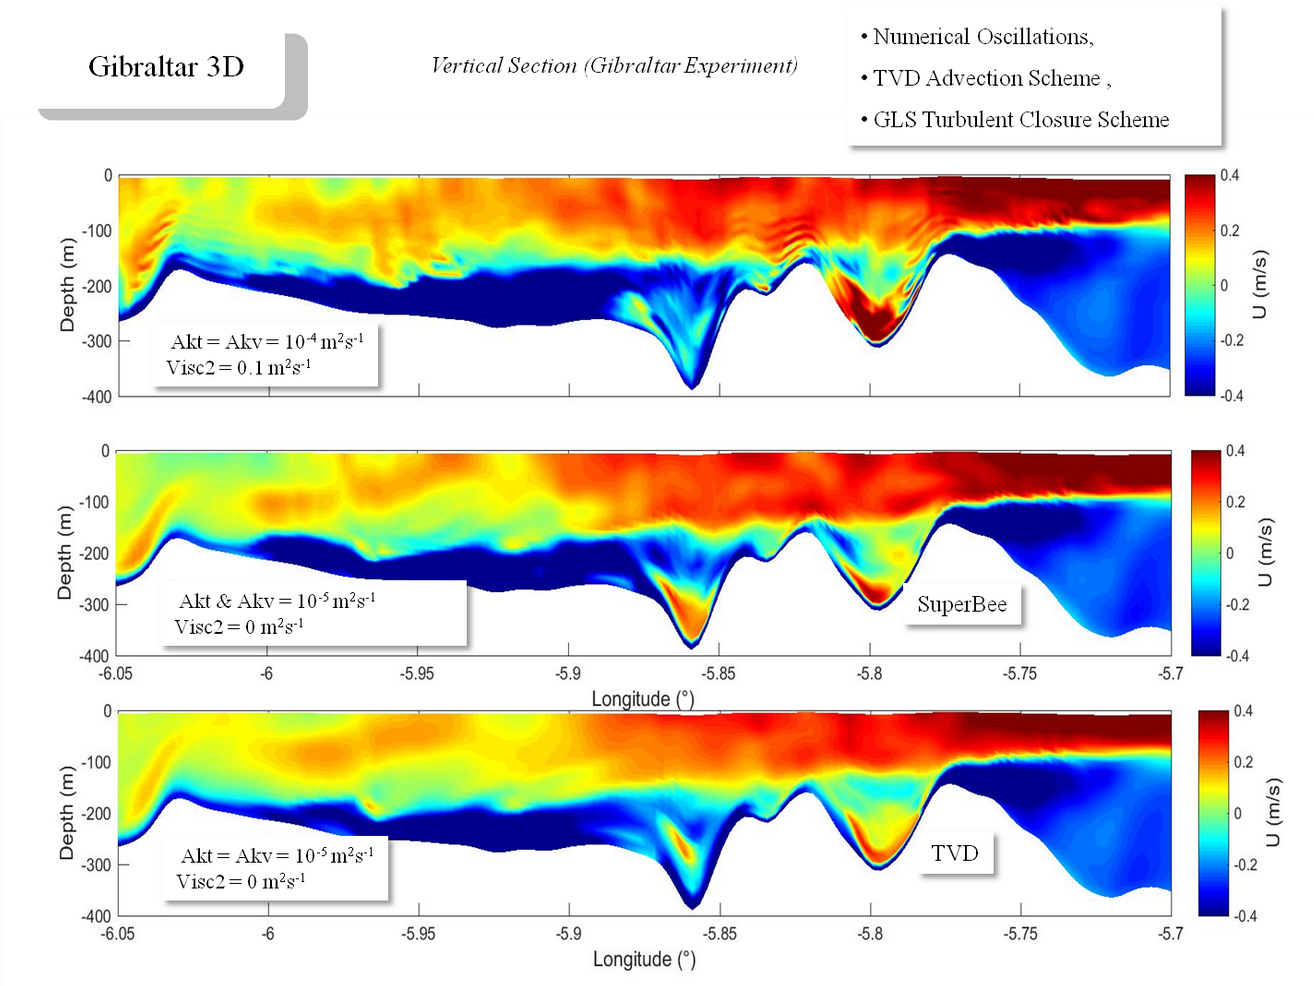
\includegraphics[width=6.29in,height=3.55in]{./media/TVD4.png}
		\caption{ : Test de sensibilité du champ de vitesse horizontale aux schémas d’advection de la quantité de mouvement. (haut) Section verticale du champ de vitesse horizontale à t=1.36T dans la maquette 3DUP3-SPLINES. (milieu) Section verticale du champ de vitesse horizontale à t=1.36 T dans la maquette 3DTVD-SUPERBEE. (bas) Section verticale du champ de vitesse horizontale à t=1.36T dans la maquette 3DTVD-MINMOD.}
		\label{Fig_TVD4}
		%\label{fig:_Test_de_sensibilit_du_champ_de_vitesse_horizontale_aux_schmas_dadvection_de_la_quantit_de_mouvement_haut_Section_verticale_du_champ_de_vitesse_horizontale__t136T_dans_la_maquette_3DUP3SPLINES_milieu_Section_verticale_du_champ_de_vitesse_horizontale__t136T_dans_la_maquette_3DTVDSUPERBEE_bas_Section_verticale_du_champ_de_vitesse_horizontale__t136T_dans_la_maquette_3DTVDMINMOD}
	\end{Center}
\end{figure}


%%%%%%%%%%%%%%%%%%%% Figure/Image No: 4 Ends here %%%%%%%%%%%%%%%%%%%%

\par

\par

\begin{justify}
Anticipant sur la section (\ref{section3DNHREF}) dédiée à la maquette NH-REF et par soucis de cohérence, nous évaluons maintenant l’impact de ces nouveaux schémas numériques sur la propagation des trains d’ondes solitaires dans la simulation 3D-NH REF : sur la Figure \ref{Fig_TVD5}, on observe que les schémas d’advection de type TVD (MINMOD, VanLeer $\&$  SUPERBEE) ont tendance à dissiper un peu plus les ondes solitaires que les schémas d’advection UP3 et SPLINES (amplitude et vitesse verticale associé aux solitons plus faibles). Cependant, l’utilisation du limiteur SUPERBEE permet de réduire significativement ces effets dissipatifs. Une nouvelle version des schémas d’advection TVD moins dissipative est actuellement en développement.
\end{justify}\par


%%%%%%%%%%%%%%%%%%%% Figure/Image No: 5 starts here %%%%%%%%%%%%%%%%%%%%

\begin{figure}[!h]
	\begin{Center}
		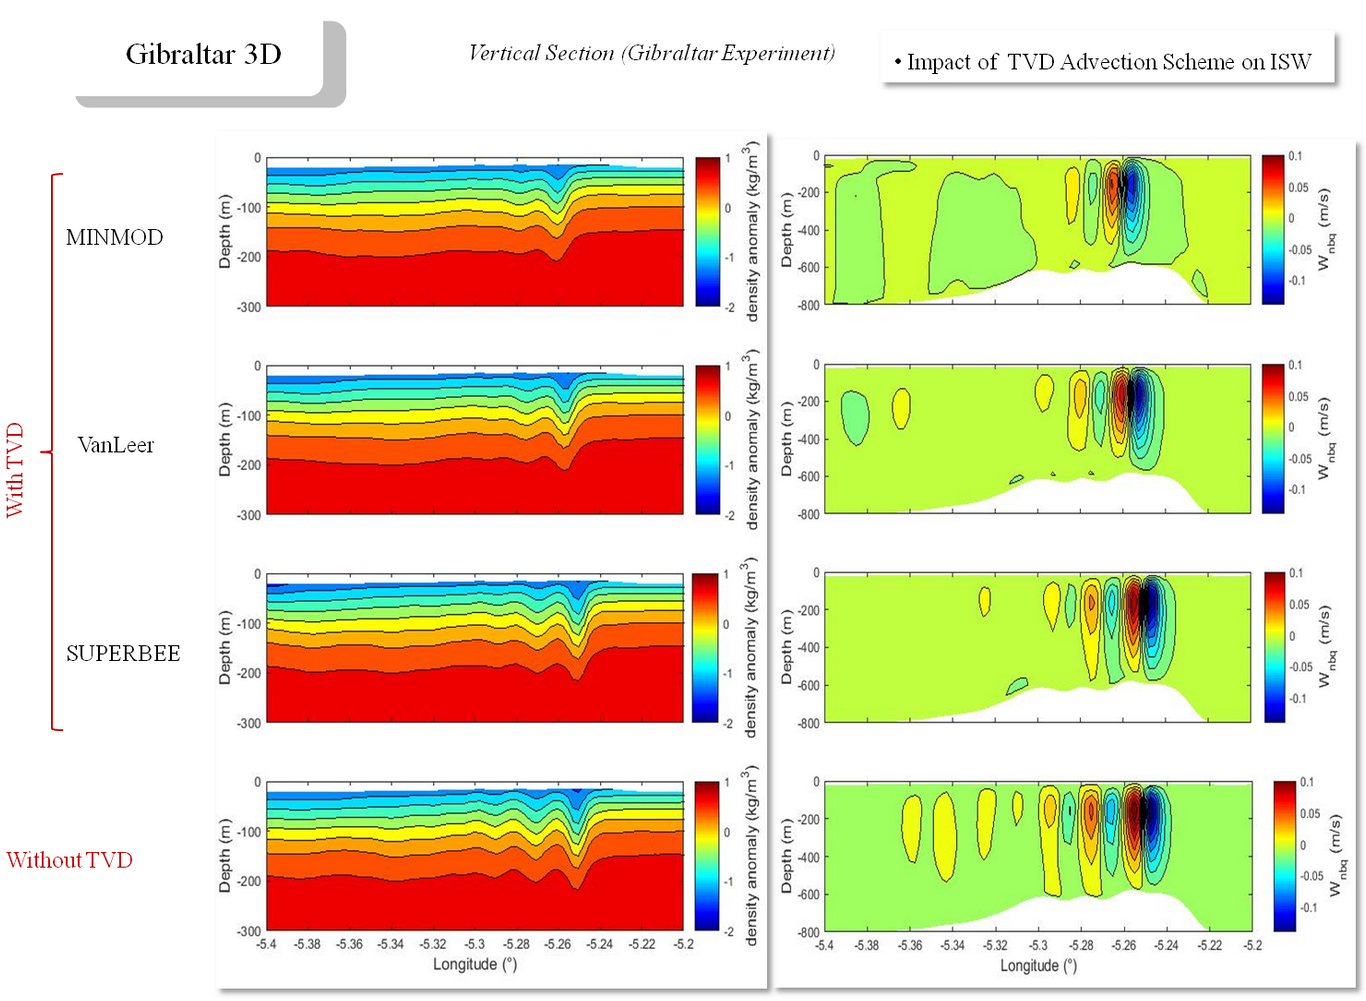
\includegraphics[width=6.3in,height=2.91in]{./media/TVD5.png}
		\caption{: Test de sensibilité des trains d’ondes solitaires aux schémas d’advection de la quantité de mouvement.\ \ \ \ \ \   Sections verticales des champs d’anomalie de densité et de vitesse verticale à t=1.1T : (a)  pour la maquette 3DTVD-MINMOD, (b) pour la maquette 3DTVD-VanLeer,\  (c)  pour la maquette 3DTVD-SUPERBEE, (d) pour la maquette 3DUP3-SPLINES.}
		\label{Fig_TVD5}
		%\label{fig:_Test_de_sensibilit_des_trains_dondes_solitaires_aux_schmas_dadvection_de_la_quantit_de_mouvement________Sections_verticales_des_champs_danomalie_de_densit_et_de_vitesse_verticale__t11T_a__pour_la_maquette_3DTVDMINMOD_b_pour_la_maquette_3DTVDVanLeer__c__pour_la_maquette_3DTVDSUPERBEE_d_pour_la_maquette_3DUP3SPLINES}
	\end{Center}
\end{figure}


%%%%%%%%%%%%%%%%%%%% Figure/Image No: 5 Ends here %%%%%%%%%%%%%%%%%%%%


%%%%%%%%%%%%%%%%%%%%%%%%%%%%%%%%%%%%%%%%%%%%%%%%%%%%%%%%%%%%%%%%%%%%%%%%%%%%%
\subsection{Discussion and conclusion}
%%%%%%%%%%%%%%%%%%%%%%%%%%%%%%%%%%%%%%%%%%%%%%%%%%%%%%%%%%%%%%%%%%%%%%%%%%%%%


In the introduction of the present study, two objectives were originally set. A first one concerns the understanding of the small-scale dynamics of the strait of Gibraltar, the other is associated to the capacity of the new time-splitting regional model CROCO-NBQ to render an easy-to-implement forecast of such a dynamics. Both objectives have been pursued in parallel and several seminal results have been obtained.

The present study confirms that both the generation of large-amplitude mode-1 and mode-2 internal waves and the onset of turbulence and its energy cascade could be simulated in the strait of Gibraltar with reasonable accuracy based on a simple, computationally efficient vertical configuration. The characteristics of the simulated internal waves compare indeed well with published observations, with numerical studies and with KdV model for ISWs. Barotropic tides are propagated with an explicit free-surface model. The mechanisms of generation, propagation and advection of mode-1 and 2 internal waves have been detailed based on maps of criticality produced for the exchange flow.
 
 To do so, a new type of non-hydrostatic non-Boussinesq algorithm (Auclair et al., 2018) had to be implemented in the otherwise numerically-efficient ROMS-CROCO and the resulting (pseudo-) compressible time-splitting code was implemented for the very first time in a realistic configuration. Sensitivity tests confirmed that a non-hydrostic (here non-Boussinesq) kernel is required (i) to simulate ISW trains and (ii) to explicitly simulate the onset of the turbulence energy cascade when (in the present case) resolution is increased from approximately 200 m to 50 m. Such small-scale turbulent structures have for instance been observed at CS by Wesson et al. (1994), where they where associated to dissipation of $10^{-2}\ W/kg$. We reached the conclusion that resolutions finer than a few hundred meters have to be associated to a refinement of the physics of the numerical kernel of the ocean code from hydrostatic to non-hydrostatic.\\
 The way the vertical configuration can be built has also been detailed with a particular attention paid to the bathymetry (implicit representation of 3D effects around isolated mounts...) and to the representation of the Coriolis pseudo-force (implicit representation of the funneling effect in the strait...). The proposed approach can now easily be implemented in other regions of the world where for instance ISW or just internal waves need to be explicitly simulated, leading to numerically-efficient forecasting tools.
 
 Vertical 2D configurations are yet limited by the representation of the velocity shear between inflowing Atlantic Waters and outflowing Mediterranean waters and more generally by the bathymetry. The inclusion of restratification process (surface and boundary forcing) would allow the model to remain accurate for a greater number of tidal cycles. The chosen Lock-exchange-like initialization additionally requires a rather long spin-up period but it provides a simple strategy to initialize a configuration with crude information on the stratification. In the present case, only two vertical profiles of temperature and salinity are required (one per variable and per water mass).
 
 The absence of transverse effects in the strait could be at least partly simulated by re-considering the definition of Coriolis pseudo-force. However several remaining processes could not be taken into account: the transverse propagation of ISWs in the strait of Gibraltar (S\'anchez'Garrido et al., 2011 and Vlasenko et al., 2009) and furthermore in the Alboran Sea, the hydraulic control in TN (Farmer and Armi, 1988, Sannino et al., 2009) or the boiling-water over CS (Bruno et al., 2002), the reflexion onto the Moroccan coast... Only the ``onset'' of the turbulence cascade could be simulated based on primary Kelvin-Helmholtz instabities. The simulation of the following secondary instabilities and down the road, the resulting energy cascade as well as the long term impact on Mediterranean and North Atlantic circulation of the refined representation of the dynamics of the strait both require a fully 3D approach which is possible with CROCO-NBQ. 
 

% Shortcomings:
% \begin{itemize}
% \item{subsection must e in pivilged diection of propagation }
% \item{
%One limitation of our testing is the lock exchange initialization that uses profiles of two water masses depicted in figure \ref{fig_LEx}. In reality, more than one water mass enter the Strait of Gibraltar on both the Atlantic and Mediterranean side. On the Mediterranean side, water masses are intermediate waters such as LIW, and also deep waters formed by deep convection that can get sucked over the sill, whereas on the Atlantic side... The mixing of the different water masses affects biogeochemical transport to the eastern end of the Srait... (macias 2006) }
%\item{3D effects/phenomena absent : control in TN, 'boiling-water' in neap-tide, reflexion on Moroccan coast, etc...3D turbulent cascade }
%\item{no restratification process}
%\item{difficulty with velocity shear}
%\end{itemize}

 \color{black}

\clearpage
%%%%%%%%%%%%%%%%%%%%%%%%%%%%%%%%%%%%%%%%%%%%%%%%%%%%%%%%%%%%%%%%%%%%%%%%%%%%%
\subsection{Appendix : computation of a Froude number}
%%%%%%%%%%%%%%%%%%%%%%%%%%%%%%%%%%%%%%%%%%%%%%%%%%%%%%%%%%%%%%%%%%%%%%%%%%%%%
Froude number for the mode-n internal wave $F_n$ is defined as $F_n=U/c^*_n$ with c$^*_n$ the linear internal wave speed of the mode-n internal wave.
 $c^*_n=\omega / k_n = \sqrt{g'h}/n$
 where $\omega$ is the wave frequency, here the M2-tidal frequency, and 
\begin{equation}
\label{eqK}
k_n=\pm \frac{n \pi}{H} \left( \frac{\omega^2 - f^2}{N^2 - \omega^2} \right) ^{1/2} 
\end{equation}

This expression of k$_n$ is derived from the linear propagation equation (Gill, 1982) derived from the Navier-Stokes conservation of momentum equations (see subsection \ref{NavierStokes}):
\begin{equation}
 W'' + k^2 \frac{N^2 - \omega^2}{\omega ^2 - f^2}W = 0
\end{equation}
with bottom and surface boundary conditions $w(0) = 0$ and $w(-H) = 0$. This expression of W$_n$ gives the structures of the vertical modes. N is chosen as the average stratification of the water column and its expression is given by equation (\ref{eqN}). 

\begin{figure}[!h]
\centering
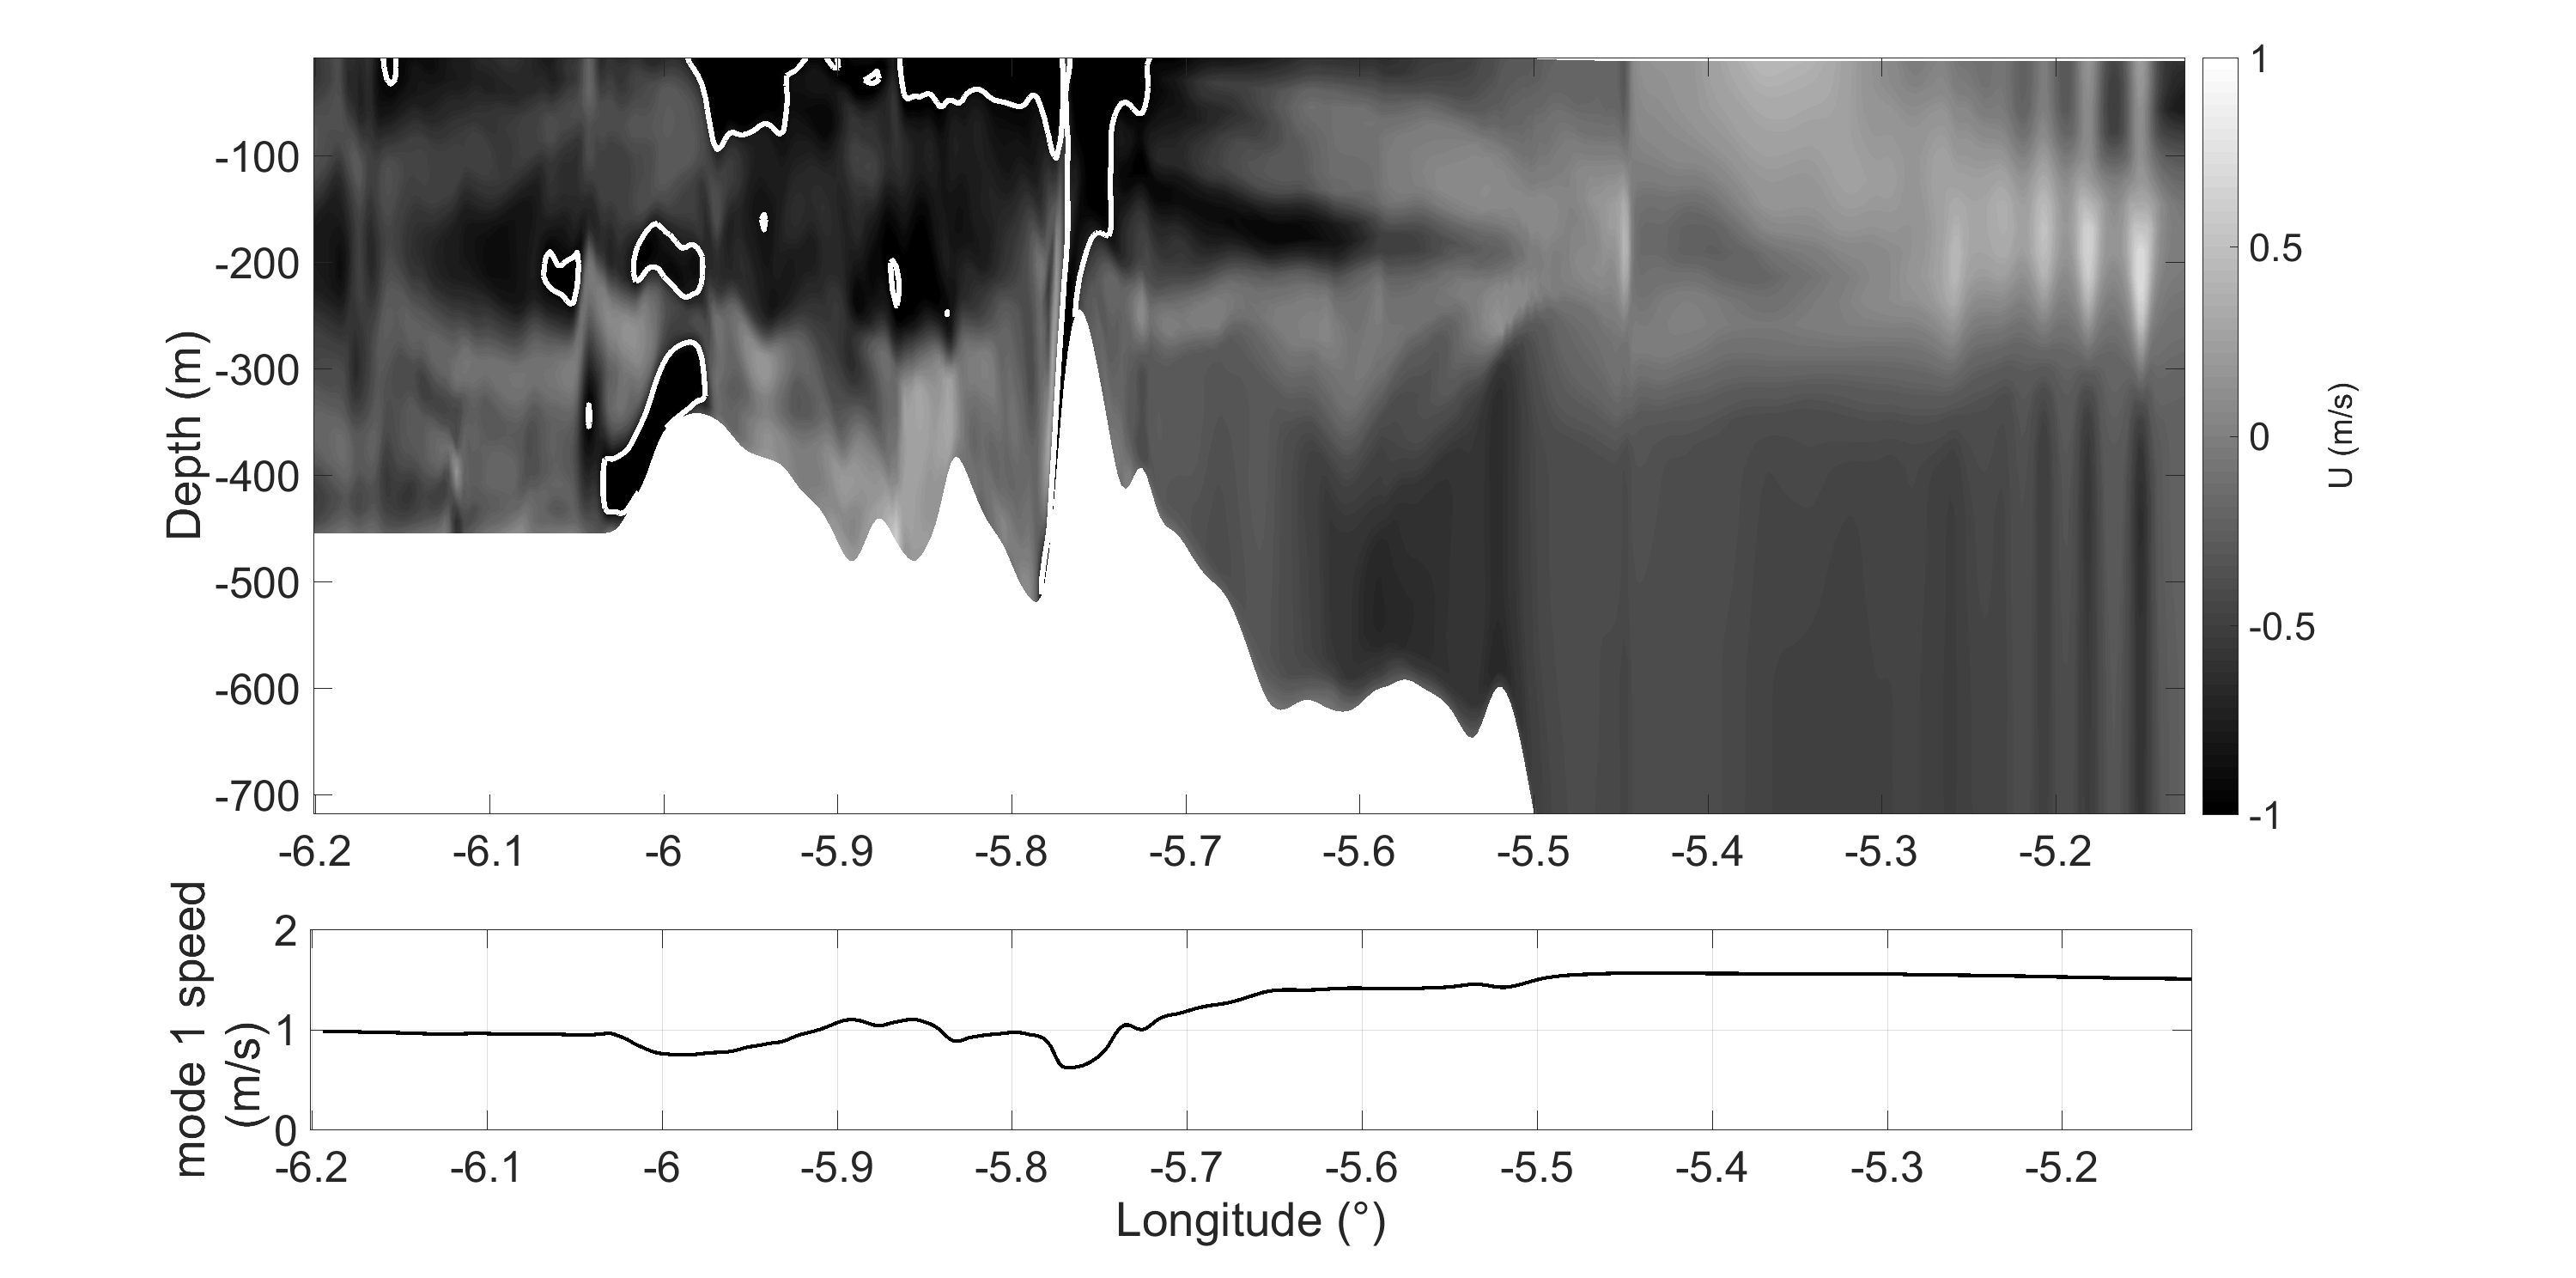
\includegraphics[width=1\linewidth]{./papier2D/comp_fn_strat.png}
\caption{Top panel : field of longitudinal velocity ($u (x,z)$) at $t = 8.5\ T$ with contour of mode 1 supercritical region (F>1) calculated from a 3T-averaged stratification . Bottom panel : Computed linear speed of mode 1 internal waves ($c^*_1 (x)$) from a 3T-averaged stratification in configuration \textbf{SimRef}.}
\label{fig_annexeF}
\end{figure}

 A value $N (x)$ is computed for the water column at each horizontal point of the subsection from a 3T averaged stratification in \textbf{SimRef}. The propagation speed for mode 1 linear waves ($c^*_1 (x)$) is then computed as $c^*_1 (x) =\omega / k_1 (x)$ with $\omega$ the pulsation of the M2-tidal component and $k_1 (x)$ from (\ref{eqK}). This value is indicated in the lower panel of figure \ref{fig_annexeF}, then compared to the field $u(x,z)$ of longitudinal velocity at t=8.5 T plotted in the upper panel. In the upper panel is also highlighted the areas where $u(x,z) > c^*_1 (x)$, hence where the Froude number $F_1$ is superior to 1. The flow inside those contours is called supercritical.
%$N$ can be calculated either from the instantaneous stratification or from a representative one. In figure \ref{fig_annexeF}, the computing of $N$ has been realized either from the field of relative density at t=8.5 T or from a 3T averaged stratification in \textbf{SimRef}. The propagation speed for mode 1 linear waves ($c^*_1$) is then computed and compared to the field of longitudinal velocity at t=8.5 T. 

%There is little difference between the two resulting mapping of supercritical flow. The positions of hydraulic controls at the sills is respected. Only the extent of the areas of F>1 is slightly lesser when based on instantaneous stratification.\color{red}Retirer cette phrase? ou la comparaison tout court...\color{black} As such, we chose to compute Froude numbers from averaged stratification in the present work.

%\color{red}Here we chose to calculate $N$ from the 3T averaged stratification in \textbf{SimRef} visible in figure \ref{fig_fn_ref}.\color{black}
%%%%%%% Biblio

%\newpage
%\nocite{Baines1995}
%\nocite{BS84}
%\nocite{FA1988}
%\nocite{FA1986}
%\nocite{Garett90}
%\nocite{Vazquez2006}
%\nocite{SG2011}
%%\nocite{Sannino2014}
%\nocite{Naranjo2014}
%\nocite{Sannino2009}
%\nocite{Sannino2009b}
%\nocite{Brandt1996}
%\nocite{Sannino2004}
%\nocite{S2005}
%\nocite{Izquierdo2001}
%\nocite{Auclair2018}
%\nocite{SN2015}
%\nocite{CW90}
%\nocite{Beth79}
%\nocite{Bray95}
%\nocite{Sannino2002}
%\nocite{FA1988}
%\nocite{Bormans1989}
%\nocite{Vlasenko2009}
%\nocite{Bryden94}
%\nocite{SG2008}
%\nocite{Wesson94}
%\nocite{Dossmann2012}
%\nocite{Grinstein2007}
%\nocite{Bruno2002}
%\nocite{tpxo8}
%\nocite{alpers85}
%\nocite{Debreu2012}

%%\begin{multicols}{2}
%\bibliographystyle{plain}
%\bibliography{./papier2D/biblio_gib}
%%\end{multicols}

 
\selectlanguage{french}

\newpage

%%%%%%%%%%%%%%%%%%%%%%%%%%%%%%%%%%%%%%%%%%%%%%%%%%%%%%%%%%%%%%%%%%%
%%%%%%%%%%%%%%%%%%%%%%%%%%%%%%%%%%%%%%%%%%%%%%%%%%%%%%%%%%%%%%%%%%%
%%% Maquettes 3D NH-HR
%%%%%%%%%%%%%%%%%%%%%%%%%%%%%%%%%%%%%%%%%%%%%%%%%%%%%%%%%%%%%%%%%%%
%%%%%%%%%%%%%%%%%%%%%%%%%%%%%%%%%%%%%%%%%%%%%%%%%%%%%%%%%%%%%%%%%%%
\section{Maquette 3D NH-REF \textit{(Tâche 1.1)}}
\label{section3DNHREF}

\noindent\fbox{\noindent\begin{minipage}{1\textwidth}
\noindent La maquette tri-dimensionnelle NH-REF est, comme son nom l'indique, la maquette de référence implémentée et exploitée dans le cadre du présent contrat. Cette maquette s'appuie sur le coeur non-hydrostatique et non-Boussinesq CROCO et sur des schémas d'advection d'ordre élevé. Elle a permis de mettre en place une première simulation des "fines échelles" pour un faible coût de calcul. La dynamique 3D ainsi simulée a confirmé les caractéristiques des processus et autres mécanismes mis en évidence par Bordois (2015) à partir d'une section verticale le long du transect principal de la campagne \textit{"Gibraltar Experiment"}. Une évaluation de la pertinence de la marée barotrope simulée a plus particulièrement été réalisée. Les caractéristiques du ressaut hydraulique et des trains d'ondes solitaires ont dans un second temps été confrontées aux observations disponibles dans la région du détroit. La variabilité de ces processus à l'amplitude de la marée a été étudiée.
\end{minipage}
}

\bigskip\bigskip
\noindent Les résultats présentés dans la section (\ref{chapitremodele}.\ref{section3DNHREF}) donnent lieu à la rédaction d'un manuscrit. Lucie Bordois aidée par l'équipe de développement du GdR CROCO est en charge de la soumission prochaine de ce manuscrit pour publication dans un journal international de rang A. Le reste de la section est donc proposé en anglais.
%%%%%%%%%%%%%%%%%%%%%%%%%%%%%%%%%%%%%%%%%%%%%%%%%%%%%%%%%%%%%%%%%%%
%%%debut article NH-REF Lucie
%%%%%%%%%%%%%%%%%%%%%%%%%%%%%%%%%%%%%%%%%%%%%%%%%%%%%%%%%%%%%%%%%%%
\selectlanguage{english}
%%%%%%%%%%%%  Generated using docx2latex.com  %%%%%%%%%%%%%%

%%%%%%%%%%%%  v2.0.0-beta  %%%%%%%%%%%%%%

%\documentclass[12pt]{report}
%\usepackage{amsmath}
%\usepackage{latexsym}
%\usepackage{amsfonts}
%\usepackage[normalem]{ulem}
%\usepackage{array}
%\usepackage{amssymb}
%\usepackage{graphicx}
%\usepackage[backend=biber,
%style=numeric,
%sorting=none,
%isbn=false,
%doi=false,
%url=false,
%]{biblatex}\addbibresource{bibliography.bib}

%\usepackage{subfig}
%\usepackage{wrapfig}
%\usepackage{wasysym}
%\usepackage{enumitem}
%\usepackage{adjustbox}
%\usepackage{ragged2e}
%\usepackage[svgnames,table]{xcolor}
%\usepackage{tikz}
%\usepackage{longtable}
%\usepackage{changepage}
%\usepackage{setspace}
%\usepackage{hhline}
%\usepackage{multicol}
%\usepackage{tabto}
%\usepackage{float}
%\usepackage{multirow}
%\usepackage{makecell}
%\usepackage{fancyhdr}
%\usepackage[toc,page]{appendix}
%\usepackage[hidelinks]{hyperref}
%\usetikzlibrary{shapes.symbols,shapes.geometric,shadows,arrows.meta}
%\tikzset{>={Latex[width=1.5mm,length=2mm]}}
%\usepackage{flowchart}\usepackage[paperheight=11.69in,paperwidth=8.27in,left=0.98in,right=0.98in,top=0.98in,bottom=0.98in,headheight=1in]{geometry}
%\usepackage[utf8]{inputenc}
%\usepackage[T1]{fontenc}
%\TabPositions{0.5in,1.0in,1.5in,2.0in,2.5in,3.0in,3.5in,4.0in,4.5in,5.0in,5.5in,6.0in,}

%\urlstyle{same}


 %%%%%%%%%%%%  Set Depths for Sections  %%%%%%%%%%%%%%

% 1) Section
% 1.1) SubSection
% 1.1.1) SubSubSection
% 1.1.1.1) Paragraph
% 1.1.1.1.1) Subparagraph


%\setcounter{tocdepth}{5}
%\setcounter{secnumdepth}{5}


 %%%%%%%%%%%%  Set Depths for Nested Lists created by \begin{enumerate}  %%%%%%%%%%%%%%

\setlistdepth{9}
\renewlist{enumerate}{enumerate}{9}
		\setlist[enumerate,1]{label=\arabic*)}
		\setlist[enumerate,2]{label=\alph*)}
		\setlist[enumerate,3]{label=(\roman*)}
		\setlist[enumerate,4]{label=(\arabic*)}
		\setlist[enumerate,5]{label=(\Alph*)}
		\setlist[enumerate,6]{label=(\Roman*)}
		\setlist[enumerate,7]{label=\arabic*}
		\setlist[enumerate,8]{label=\alph*}
		\setlist[enumerate,9]{label=\roman*}

\renewlist{itemize}{itemize}{9}
		\setlist[itemize]{label=$\cdot$}
		\setlist[itemize,1]{label=\textbullet}
		\setlist[itemize,2]{label=$\circ$}
		\setlist[itemize,3]{label=$\ast$}
		\setlist[itemize,4]{label=$\dagger$}
		\setlist[itemize,5]{label=$\triangleright$}
		\setlist[itemize,6]{label=$\bigstar$}
		\setlist[itemize,7]{label=$\blacklozenge$}
		\setlist[itemize,8]{label=$\prime$}

 %%%%%%%%%%%%  Header here  %%%%%%%%%%%%%%
%\pagestyle{fancy}
%\fancyhf{}
%\renewcommand{\headrulewidth}{0pt}
%\setlength{\topsep}{0pt}\setlength{\parindent}{0pt}
%\renewcommand{\arraystretch}{1.3}

%%%%%%%%%%%%%%%%%%%% Document code starts here %%%%%%%%%%%%%%%%%%%%

\vspace{\baselineskip}
\subsection{Introduction}

The Gibraltar strait system controls the exchange between the Mediterranean basin and the global ocean. In this region, large topographic variations and strong tidal currents (up to 1.8 m/s above Camarinal sill) lead to complex generation mechanisms of energetic non-linear internal waves (Vázquez et al., 2006; Vlasenko et al., 2009). The propagation of these waves is highly influenced by the complex basin geometry (Sánchez-Garrido et al., 2011) and the hydraulic criticality of the flow (Sannino, 2009; Sannino et al., 2007). These local fine-scale processes are driving turbulence levels in the order of magnitude larger than open-ocean levels (Wesson and Gregg, 1994) possibly affecting water-mass exchange (Sannino et al., 2015). The interplays of these processes with the vertical mixing and local circulation are still an ongoing scientific issue. A non-hydrostatic and non-Boussinesq model (the CROCO ocean community model) has been implemented in a realistic 3D configuration on the strait of Gibraltar area to model explicitly these fine scale processes. The 3D high resolution (220 m) model is forced by the main barotropic tidal components (i.e. M2, S2, K1, O1) through the specification of the ENEA Mediterranean-Black Sea tidal operative forecasting system solutions. It provides a good representation of the barotropic $\&$  baroclinic tides in the strait of Gibraltar, representing well the internal fine-scale activity: hydraulic jumps formation above the main sills, internal solitary wave’s generation $\&$ propagation, neap-spring tide variability... \par

\vspace{\baselineskip}
\subsection{Modeling approach}

\vspace{\baselineskip}
\subsubsection{Non-Hydrostatic, non-Boussinesq Kernel of CROCO community code}

\vspace{\baselineskip}
Simulations are performed using the free-surface non-hydrostatic and non-Boussinesq kernel of the coastal and regional ocean community model CROCO. CROCO is a new oceanic modeling system built upon ROMS-AGRIF and the non-hydrostatic kernel of SNH (Auclair et al., 2018). It solves the dynamic and thermodynamic equations using stretched, terrain-following vertical s-coordinates and orthogonal, curvilinear horizontal coordinates with a two-mode time-splitting between baroclinic and barotropic modes. For general circulation purposes, it is forced by atmospheric momentum, heat and tracer fluxes. For a more extensive description and technical details of the hydrodynamic model as well as earlier applications to the US West Coast, we refer to Shchepetkin and McWilliams (1998, 2003, 2005), Marchesiello et al. (2001, 2003) and to Penven\ et al. (2006).  \par

\vspace{\baselineskip}
The nonhydrostatic and non-Boussinesq version of CROCO uses an original two-mode time-splitting technique between barotropic (\textit{$ \Delta $ t}{\fontsize{7pt}{8.4pt}\selectfont \textit{e}}) and non-hydrostatic (\textit{$ \Delta t$}{\fontsize{7pt}{8.4pt}\selectfont \textit{NBQ}}) motions to deal with free surface, non-hydrostatic flows and acoustic waves which are explicitly simulated. In the present non-Boussinesq\ version, a time-splitting is performed to circumvent the drastic CFL criteria induced by the high phase-velocity of such waves, $c_s$. Acoustic waves or more exactly $``$pseudo-acoustic$"$\footnote{When necessary and when pertinent, acoustic-wave velocity can indeed be lowered to reduce computing costs.}  waves have indeed been re-introduced to reduce computational costs. Indeed, this avoids Boussinesq-mathematical degeneracy which inevitably requires the inversion of a 3D Poisson-system in non-hydrostatic pressure-correction methods. As long as they remain faster than the fastest physical processes in the domain, the so-called $``$pseudo-acoustic$"$ wave phase-velocity can artificially be slowed down rendering unphysical high-frequency processes associated with bulk compressibility but preserving a coherent "slow", non-hydrostatic dynamics with a softening of the CFL criterion.\par

\vspace{\baselineskip}
To model explicitly internal fine-scale turbulent processes in Gibraltar strait,  a Monotone-Integrated Large Eddy Simulation{\fontsize{11pt}{13.2pt}\selectfont  }(MILES) approach has been chosen. In MILES, the dissipative nature of some classes of advection schemes is exploited to provide an implicit model of turbulence. Small, molecular values of the kinematic viscosity ($\nu\ = 10^{-6} m^{2}/s$) and density diffusivity ($K_\rho\ = 10^{-6} m^2/s$) are used, without neither turbulence closure scheme nor additional viscosity. Numerical dissipation is provided through a Total Variation Diminishing (TVD) advection scheme for the momentum and a fifth-order WENO advection-scheme for tracers. TVD and WENO-5 schemes are modern shock-capturing schemes which allow the simulation of sharp discontinuities. The objective is obviously not to reproduce the entire turbulent cascade but to be able to resolve explicitly the largest features of the internal fines-scale turbulent processes. \par


\vspace{\baselineskip}
\subsubsection{Numerical configurations}

\vspace{\baselineskip}
A non-hydrostatic (R\textsubscript{NBQ}) and a hydrostatic (R\textsubscript{H}) simulation are performed. A 3D version of the model is used with lateral Orlanski radiation conditions and free surface boundary conditions. A constant quadratic bottom stress formulation is used with a drag coefficient of $10^{-3}$. The model domain extends from the Gulf of Cadiz to the Alboran sea (Figure \ref{Fig1_Lucie}). The horizontal grid is constant with a resolution of 220 m and the vertical model grid is based on 40 $\sigma$-levels. Initial conditions for temperature and salinity are given by the ENEA Mediterranean-Black Sea tidal operative forecasting system\footnote{http://www.enea.it/it/seguici/pubblicazioni/pdf-volumi/cresco-report-2016.pdf}. Wind and surface fluxes are not included in the simulations. Tides are incorporated through the specification at the lateral boundary for the barotropic velocity and the surface elevation. Both are given by the ENEA Mediterranean-Black Sea tidal operative forecasting system. The ENEA forecasting system provides also lateral boundary conditions for salinity, temperature and baroclinic velocities (geostrophic currents). Table \ref{Tab1_Lucie} summarizes the numerical and physical parameters of both configurations. \par

%%%%%%%%%%%%%%%%%%%% Table No: 1 starts here %%%%%%%%%%%%%%%%%%%%

\begin{table}[!h]
 			\centering
\begin{tabular}{p{1.56in}p{4.48in}}
\hline

%row no:2
\multicolumn{1}{|p{1.56in}}{(Nx, Ny, Nz, Nt) } & 
\multicolumn{1}{|p{4.48in}|}{\Centering (408, 523, 40, 669 600)} \\
\hhline{--}
%row no:3
\multicolumn{1}{|p{1.56in}}{Simulated period} & 
\multicolumn{1}{|p{4.48in}|}{\Centering [10/09/2017 – 10/10/2017]} \\
\hhline{--}
%row no:4
\multicolumn{1}{|p{1.56in}}{($ \Delta $ x, $ \Delta $ y, $ \Delta $ z) } & 
\multicolumn{1}{|p{4.48in}|}{\Centering (220 m, 220 m, 7-23 m)} \\
\hhline{--}
%row no:5
\multicolumn{1}{|p{1.56in}}{($ \Delta $ t, N\textsubscript{e}) } & 
\multicolumn{1}{|p{4.48in}|}{\Centering (4s, 9)} \\
\hhline{--}
%row no:6
\multicolumn{1}{|p{1.56in}}{Cs (for R\textsubscript{NBQ}) } & 
\multicolumn{1}{|p{4.48in}|}{\Centering 400 m/s} \\
\hhline{--}
%row no:7
\multicolumn{1}{|p{1.56in}}{Bathymetry } & 
\multicolumn{1}{|p{4.48in}|}{\Centering SHOM (500 m)} \\
\hhline{--}
%row no:8
\multicolumn{1}{|p{1.56in}}{\multirow{1}{*}{\begin{tabular}{p{1.56in}}Tidal forcing \\\end{tabular}}} & 
\multicolumn{1}{|p{4.48in}|}{\Centering ENEA Mediterranean-Black Sea tidal operative forecasting system} \\
\hhline{~-}
%row no:9
\multicolumn{1}{|p{1.56in}}{} & 
\multicolumn{1}{|p{4.48in}|}{\Centering M2, S2, K1, O1} \\
\hhline{--}
%row no:10
\multicolumn{1}{|p{1.56in}}{Stratification } & 
\multicolumn{1}{|p{4.48in}|}{\Centering ENEA Mediterranean-Black Sea tidal operative forecasting system} \\
\hhline{--}
%row no:11
\multicolumn{1}{|p{1.56in}}{Geostrophic currents } & 
\multicolumn{1}{|p{4.48in}|}{\Centering ENEA Mediterranean-Black Sea tidal operative forecasting system} \\
\hhline{--}
%row no:12
\multicolumn{1}{|p{1.56in}}{Atmospheric forcing } & 
\multicolumn{1}{|p{4.48in}|}{\Centering No} \\
\hhline{--}
%row no:13
\multicolumn{1}{|p{1.56in}}{Advection schemes } & 
\multicolumn{1}{|p{4.48in}|}{\Centering TVD (U-V-W) $\&$  WENO5 (T-S)} \\
\hhline{--}

\end{tabular}
%%%%%%%%%%%%%%%%%%%% Table No: 1 ends here %%%%%%%%%%%%%%%%%%%%

\caption{Numerical $\&$  physical parameters of \textbf{R\textsubscript{H}} and \textbf{R\textsubscript{NBQ}}}
\label{Tab1_Lucie}
\end{table}

\vspace{\baselineskip}
The bathymetry is extracted from a 500-m-resolution topographic data set of the Strait of Gibraltar provided from the SHOM (HOMONIM 500-m-Grid). A Gaussian interpolation of the topography data has been made\footnote{Parameters of the Gaussian interpolation: Gaussian radius: $r_{max}\ =\ 0.25$, minimum depth $h_{min}\ =\ 30\ m$.} to set up the 220-m-grid. The resulting model bathymetry is illustrated on figure \ref{Fig1_Lucie}.a. On the vertical section of figure \ref{Fig1_Lucie}.b, the dominant topographic features of the strait are clearly recognizable (from west to east): Espartel sill (ES); Tangier basin (TB); Camarinal sill (CS), with the minimum depth of 188 m, and Tarifa Narrows (TN) with the maximum depth of 960 m. This vertical section (located by the black line on figure \ref{Fig1_Lucie}.a) has been selected to incorporate ES, the shallowest point of CS and the deepest point of TN. The vertical resolution $(\Delta z\ =\ 7-23\ m$) is much higher above Camarinal sill than in the eastern and western ends. \par

\vspace{\baselineskip}

%%%%%%%%%%%%%%%%%%%% Figure/Image No: 1 starts here %%%%%%%%%%%%%%%%%%%%

\begin{figure}[!h]
	\begin{Center}
		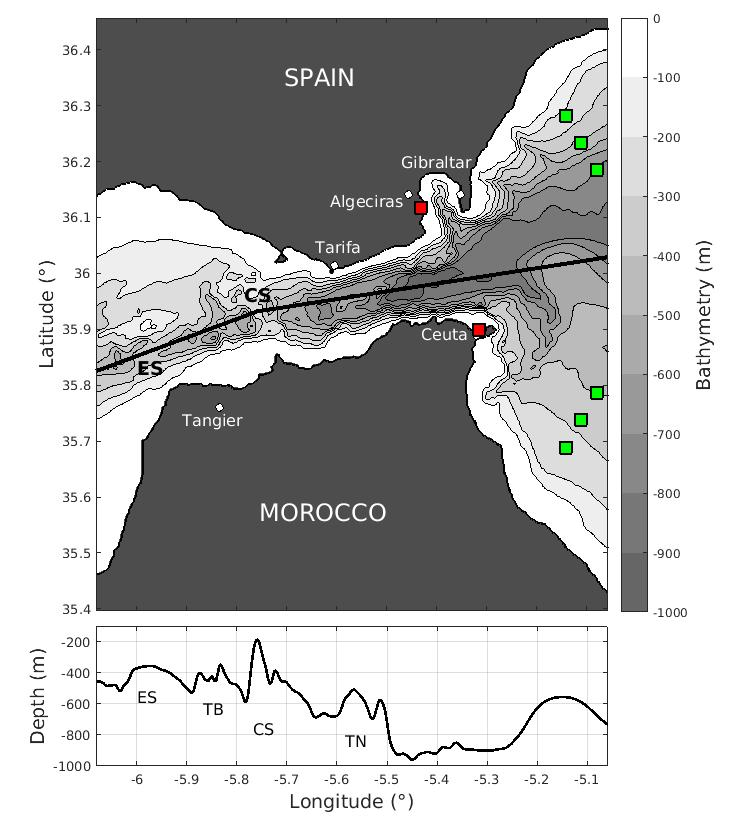
\includegraphics[width=3.77in,height=4.44in]{./media/image1.jpg}
	\end{Center}

%%%%%%%%%%%%%%%%%%%% Figure/Image No: 1 Ends here %%%%%%%%%%%%%%%%%%%%

\caption { Bathymetry and domain extension of R\textsubscript{NBQ} $\&$  R\textsubscript{H}. The black line locate the vertical transect/section on the lower plot. Red squares locate tidal gauges position and green squares locate Xtrack position.}
 \label{Fig1_Lucie}
\end{figure}

\vspace{\baselineskip}
\subsection{Barotropic tides}

\vspace{\baselineskip}
Barotropic tides in the region present an original pattern due to the complex geometry of the strait and its strong dynamics. The tides are typically semi-diurnal, as in the whole Northern Atlantic Ocean, and flowing back and forth zonally at a first glance. The large tidal flows at the Atlantic entrance are strongly reduced in the strait to enter the Mediterranean Sea with typical amplitudes of a few tens of centimeters. The adjustment of the flow imposes complex tidal patterns into the Strait itself making the modelling of barotropic tides in the strait region very challenging. \\
This complexity is circumvented in state-of-the-art barotropic tidal models thanks to the assimilation of altimeter data particularly. But, into the Strait, the lack of data to constrain the cotidal charts makes these global models very precise outside the Strait but less inside. So the forcing they can impose at the boundary of a reduced modelling domain centered on the Strait is generally an important source of error. A huge modelling effort is thus necessary to assess the sensitivity of CROCO to various parameters (bathymetry, open-boundary conditions, forcing atlas...). Additional work (eg. bathymetry, bottom friction, large-scale forcing compatibility, ... ) will be needed to overcome the remaining difficulties.\\
Both configurations (R\textsubscript{NBQ} $\&$  R\textsubscript{H}) run over two spring neap cycles, and the results are compared with available observed data (X-TRACK altimetry and tidal gauges). \par
In Tables \ref{Tab1_Lucie}, \ref{Tab2_Lucie} and \ref{Tab3_Lucie} the observed and simulated amplitudes ($A$) and phases ($G$) are compared for the
main barotropic tidal components (M2, S2, K1, O1). As expected, the simulated amplitudes ($A$) and phases ($G$) of the four tidal components are very similar in the hydrostatic and non-hydrostatic runs.\\

A good agreement between observed and predicted values is found; the maximum differences do not exceed 4.8 cm in amplitude and 11.3° in phase for the semi-diurnal components. The relative errors (dE/A) are significant for the diurnal components (O1, K1), however the amplitudes of these components are quite small in that region.


%%%%%%%%%%%%%%%%%%%% Table No: 2 starts here %%%%%%%%%%%%%%%%%%%%


\begin{table}[!h]
 			\centering
\begin{tabular}{p{0.25in}p{0.31in}p{0.54in}p{0.54in}p{0.54in}p{0.5in}p{0.54in}p{0.54in}p{0.54in}p{0.5in}}
\hline
%row no:1
\multicolumn{2}{|p{0.56in}}{\Centering {\fontsize{11pt}{13.2pt}\selectfont Simulation}} & 
\multicolumn{4}{|p{2.12in}}{\Centering {\fontsize{11pt}{13.2pt}\selectfont R\textsubscript{NBQ}}} & 
\multicolumn{4}{|p{2.12in}|}{\Centering {\fontsize{11pt}{13.2pt}\selectfont R\textsubscript{H}}} \\
\hhline{----------}
%row no:2
\multicolumn{2}{|p{0.56in}}{\cellcolor[HTML]{EFEFEF}} & 
\multicolumn{1}{|p{0.54in}}{\cellcolor[HTML]{EFEFEF}\Centering {\fontsize{11pt}{13.2pt}\selectfont dA (cm)}} & 
\multicolumn{1}{|p{0.54in}}{\cellcolor[HTML]{EFEFEF}\Centering {\fontsize{11pt}{13.2pt}\selectfont dG ($ ^{\circ} $)}} & 
\multicolumn{1}{|p{0.54in}}{\cellcolor[HTML]{EFEFEF}\Centering {\fontsize{11pt}{13.2pt}\selectfont $ \vert\vert dE \vert\vert$  (cm)}} & 
\multicolumn{1}{|p{0.5in}}{\cellcolor[HTML]{EFEFEF}\Centering {\fontsize{11pt}{13.2pt}\selectfont \Tiny{\textbf{$ \vert\vert dE \vert\vert/A$ ($\%$ )}}}} & 
\multicolumn{1}{|p{0.54in}}{\cellcolor[HTML]{EFEFEF}\Centering {\fontsize{11pt}{13.2pt}\selectfont dA (cm)}} & 
\multicolumn{1}{|p{0.54in}}{\cellcolor[HTML]{EFEFEF}\Centering {\fontsize{11pt}{13.2pt}\selectfont dG ($ ^{\circ} $)}} & 
\multicolumn{1}{|p{0.54in}}{\cellcolor[HTML]{EFEFEF}\Centering {\fontsize{11pt}{13.2pt}\selectfont $ \vert\vert dE \vert\vert$ (cm)}} & 
\multicolumn{1}{|p{0.5in}|}{\cellcolor[HTML]{EFEFEF}\Centering {\fontsize{11pt}{13.2pt}\selectfont \Tiny{\textbf{$ \vert\vert dE \vert\vert/A$ ($\%$ )}}}} \\
\hhline{----------}
%row no:3
\multicolumn{1}{|p{0.25in}}{\multirowcell{}{}{\begin{tabular}{p{0.16in}}\Centering {\fontsize{11pt}{13.2pt}\selectfont M2}\\\end{tabular}}} & 
\multicolumn{1}{|p{0.31in}}{\Centering {\fontsize{11pt}{13.2pt}\selectfont North}} & 
\multicolumn{1}{|p{0.54in}}{\Centering {\fontsize{9pt}{10.8pt}\selectfont 4.8+-0.7}} & 
\multicolumn{1}{|p{0.54in}}{\Centering {\fontsize{9pt}{10.8pt}\selectfont 0.7+-3.6}} & 
\multicolumn{1}{|p{0.54in}}{\Centering {\fontsize{9pt}{10.8pt}\selectfont 3.4+-1.2}} & 
\multicolumn{1}{|p{0.5in}}{\Centering {\fontsize{10pt}{12.0pt}\selectfont \textbf{15.3}}} & 
\multicolumn{1}{|p{0.54in}}{\Centering {\fontsize{9pt}{10.8pt}\selectfont 4.8+-0.7}} & 
\multicolumn{1}{|p{0.54in}}{\Centering {\fontsize{9pt}{10.8pt}\selectfont 0.3+-3.6}} & 
\multicolumn{1}{|p{0.54in}}{\Centering {\fontsize{9pt}{10.8pt}\selectfont 3.4+-1.2}} & 
\multicolumn{1}{|p{0.5in}|}{\Centering {\fontsize{10pt}{12.0pt}\selectfont \textbf{15.3}}} \\
\hhline{~---------}
%row no:4
\multicolumn{1}{|p{0.25in}}{} & 
\multicolumn{1}{|p{0.31in}}{\Centering {\fontsize{11pt}{13.2pt}\selectfont South}} & 
\multicolumn{1}{|p{0.54in}}{\Centering {\fontsize{9pt}{10.8pt}\selectfont 4.5+-0.7}} & 
\multicolumn{1}{|p{0.54in}}{\Centering {\fontsize{9pt}{10.8pt}\selectfont -10.6+-4.4}} & 
\multicolumn{1}{|p{0.54in}}{\Centering {\fontsize{9pt}{10.8pt}\selectfont 4.3+-1.4}} & 
\multicolumn{1}{|p{0.5in}}{\Centering {\fontsize{10pt}{12.0pt}\selectfont \textbf{19.5}}} & 
\multicolumn{1}{|p{0.54in}}{\Centering {\fontsize{9pt}{10.8pt}\selectfont 4.4+-0.7}} & 
\multicolumn{1}{|p{0.54in}}{\Centering {\fontsize{9pt}{10.8pt}\selectfont -11.1+-4.4}} & 
\multicolumn{1}{|p{0.54in}}{\Centering {\fontsize{9pt}{10.8pt}\selectfont 4.4+-1.5}} & 
\multicolumn{1}{|p{0.5in}|}{\Centering {\fontsize{10pt}{12.0pt}\selectfont \textbf{19.6}}} \\
\hhline{----------}
%row no:5
\multicolumn{1}{|p{0.25in}}{\multirow{1}{*}{\begin{tabular}{p{0.16in}}\cellcolor[HTML]{EFEFEF}\Centering {\fontsize{11pt}{13.2pt}\selectfont S2}\\\end{tabular}}} & 
\multicolumn{1}{|p{0.31in}}{\cellcolor[HTML]{EFEFEF}\Centering {\fontsize{11pt}{13.2pt}\selectfont North}} & 
\multicolumn{1}{|p{0.54in}}{\cellcolor[HTML]{EFEFEF}\Centering {\fontsize{9pt}{10.8pt}\selectfont 0.1+-2}} & 
\multicolumn{1}{|p{0.54in}}{\cellcolor[HTML]{EFEFEF}\Centering {\fontsize{9pt}{10.8pt}\selectfont 11.3+-16}} & 
\multicolumn{1}{|p{0.54in}}{\cellcolor[HTML]{EFEFEF}\Centering {\fontsize{9pt}{10.8pt}\selectfont 0.9+-2}} & 
\multicolumn{1}{|p{0.5in}}{\cellcolor[HTML]{EFEFEF}\Centering {\fontsize{10pt}{12.0pt}\selectfont \textbf{24}}} & 
\multicolumn{1}{|p{0.54in}}{\cellcolor[HTML]{EFEFEF}\Centering {\fontsize{9pt}{10.8pt}\selectfont 0.2+-1.8}} & 
\multicolumn{1}{|p{0.54in}}{\cellcolor[HTML]{EFEFEF}\Centering {\fontsize{9pt}{10.8pt}\selectfont 11.3+-16}} & 
\multicolumn{1}{|p{0.54in}}{\cellcolor[HTML]{EFEFEF}\Centering {\fontsize{9pt}{10.8pt}\selectfont 0.8+-1.9}} & 
\multicolumn{1}{|p{0.5in}|}{\cellcolor[HTML]{EFEFEF}\Centering {\fontsize{10pt}{12.0pt}\selectfont \textbf{23.5}}} \\
\hhline{~---------}
%row no:6
\multicolumn{1}{|p{0.25in}}{\cellcolor[HTML]{EFEFEF}} & 
\multicolumn{1}{|p{0.31in}}{\cellcolor[HTML]{EFEFEF}\Centering {\fontsize{11pt}{13.2pt}\selectfont South}} & 
\multicolumn{1}{|p{0.54in}}{\cellcolor[HTML]{EFEFEF}\Centering {\fontsize{9pt}{10.8pt}\selectfont 1.2+-0.9}} & 
\multicolumn{1}{|p{0.54in}}{\cellcolor[HTML]{EFEFEF}\Centering {\fontsize{9pt}{10.8pt}\selectfont -5.5+-3}} & 
\multicolumn{1}{|p{0.54in}}{\cellcolor[HTML]{EFEFEF}\Centering {\fontsize{9pt}{10.8pt}\selectfont 1+-0.7}} & 
\multicolumn{1}{|p{0.5in}}{\cellcolor[HTML]{EFEFEF}\Centering {\fontsize{10pt}{12.0pt}\selectfont \textbf{14.1}}} & 
\multicolumn{1}{|p{0.54in}}{\cellcolor[HTML]{EFEFEF}\Centering {\fontsize{9pt}{10.8pt}\selectfont 1.2+1.0}} & 
\multicolumn{1}{|p{0.54in}}{\cellcolor[HTML]{EFEFEF}\Centering {\fontsize{9pt}{10.8pt}\selectfont -6.0+-3}} & 
\multicolumn{1}{|p{0.54in}}{\cellcolor[HTML]{EFEFEF}\Centering {\fontsize{9pt}{10.8pt}\selectfont 1+-0.7}} & 
\multicolumn{1}{|p{0.5in}|}{\cellcolor[HTML]{EFEFEF}\Centering {\fontsize{10pt}{12.0pt}\selectfont \textbf{14.3}}} \\
\hhline{----------}
%row no:7
\multicolumn{1}{|p{0.25in}}{\multirow{1}{*}{\begin{tabular}{p{0.16in}}\Centering {\fontsize{11pt}{13.2pt}\selectfont K1}\\\end{tabular}}} & 
\multicolumn{1}{|p{0.31in}}{\Centering {\fontsize{11pt}{13.2pt}\selectfont North}} & 
\multicolumn{1}{|p{0.54in}}{\Centering {\fontsize{9pt}{10.8pt}\selectfont -0.01+-0.1}} & 
\multicolumn{1}{|p{0.54in}}{\Centering {\fontsize{9pt}{10.8pt}\selectfont 2.2+-1.8}} & 
\multicolumn{1}{|p{0.54in}}{\Centering {\fontsize{9pt}{10.8pt}\selectfont 0.1+-0.7}} & 
\multicolumn{1}{|p{0.5in}}{\Centering {\fontsize{10pt}{12.0pt}\selectfont \textbf{20.4}}} & 
\multicolumn{1}{|p{0.54in}}{\Centering {\fontsize{9pt}{10.8pt}\selectfont -0.02+-1.0}} & 
\multicolumn{1}{|p{0.54in}}{\Centering {\fontsize{9pt}{10.8pt}\selectfont 0.8+-1.1}} & 
\multicolumn{1}{|p{0.54in}}{\Centering {\fontsize{9pt}{10.8pt}\selectfont 0.1+-0.7}} & 
\multicolumn{1}{|p{0.5in}|}{\Centering {\fontsize{10pt}{12.0pt}\selectfont \textbf{21.1}}} \\
\hhline{~---------}
%row no:8
\multicolumn{1}{|p{0.25in}}{} & 
\multicolumn{1}{|p{0.31in}}{\Centering {\fontsize{11pt}{13.2pt}\selectfont South}} & 
\multicolumn{1}{|p{0.54in}}{\Centering {\fontsize{9pt}{10.8pt}\selectfont -1.7+-0.8}} & 
\multicolumn{1}{|p{0.54in}}{\Centering {\fontsize{9pt}{10.8pt}\selectfont 37.8+-2.5}} & 
\multicolumn{1}{|p{0.54in}}{\Centering {\fontsize{9pt}{10.8pt}\selectfont 1.6+-0.5}} & 
\multicolumn{1}{|p{0.5in}}{\Centering {\fontsize{10pt}{12.0pt}\selectfont \textbf{66.5}}} & 
\multicolumn{1}{|p{0.54in}}{\Centering {\fontsize{9pt}{10.8pt}\selectfont -1.5+-0.8}} & 
\multicolumn{1}{|p{0.54in}}{\Centering {\fontsize{9pt}{10.8pt}\selectfont 37.8+-2.3}} & 
\multicolumn{1}{|p{0.54in}}{\Centering {\fontsize{9pt}{10.8pt}\selectfont 1.6+-0.5}} & 
\multicolumn{1}{|p{0.5in}|}{\Centering {\fontsize{10pt}{12.0pt}\selectfont \textbf{65.4}}} \\
\hhline{----------}
%row no:9
\multicolumn{1}{|p{0.25in}}{\multirow{1}{*}{\begin{tabular}{p{0.16in}}\cellcolor[HTML]{EFEFEF}\Centering {\fontsize{11pt}{13.2pt}\selectfont O1}\\\end{tabular}}} & 
\multicolumn{1}{|p{0.31in}}{\cellcolor[HTML]{EFEFEF}\Centering {\fontsize{11pt}{13.2pt}\selectfont North}} & 
\multicolumn{1}{|p{0.54in}}{\cellcolor[HTML]{EFEFEF}\Centering {\fontsize{9pt}{10.8pt}\selectfont -0.8+-0.6}} & 
\multicolumn{1}{|p{0.54in}}{\cellcolor[HTML]{EFEFEF}\Centering {\fontsize{9pt}{10.8pt}\selectfont -10.7$ \pm $ 13.6}} & 
\multicolumn{1}{|p{0.54in}}{\cellcolor[HTML]{EFEFEF}\Centering {\fontsize{9pt}{10.8pt}\selectfont 0.7+-0.5}} & 
\multicolumn{1}{|p{0.5in}}{\cellcolor[HTML]{EFEFEF}\Centering {\fontsize{10pt}{12.0pt}\selectfont \textbf{46.6}}} & 
\multicolumn{1}{|p{0.54in}}{\cellcolor[HTML]{EFEFEF}\Centering {\fontsize{9pt}{10.8pt}\selectfont -1+-0.6}} & 
\multicolumn{1}{|p{0.54in}}{\cellcolor[HTML]{EFEFEF}\Centering {\fontsize{9pt}{10.8pt}\selectfont -8.1$ \pm $ 13.0}} & 
\multicolumn{1}{|p{0.54in}}{\cellcolor[HTML]{EFEFEF}\Centering {\fontsize{9pt}{10.8pt}\selectfont 0.8+-0.5}} & 
\multicolumn{1}{|p{0.5in}|}{\cellcolor[HTML]{EFEFEF}\Centering {\fontsize{10pt}{12.0pt}\selectfont \textbf{48.8}}} \\
\hhline{~---------}
%row no:10
\multicolumn{1}{|p{0.25in}}{\cellcolor[HTML]{EFEFEF}} & 
\multicolumn{1}{|p{0.31in}}{\cellcolor[HTML]{EFEFEF}\Centering {\fontsize{11pt}{13.2pt}\selectfont South}} & 
\multicolumn{1}{|p{0.54in}}{\cellcolor[HTML]{EFEFEF}\Centering {\fontsize{10pt}{12.0pt}\selectfont 0.2+-0.5}} & 
\multicolumn{1}{|p{0.54in}}{\cellcolor[HTML]{EFEFEF}\Centering {\fontsize{10pt}{12.0pt}\selectfont -8.5+-18.5}} & 
\multicolumn{1}{|p{0.54in}}{\cellcolor[HTML]{EFEFEF}\Centering {\fontsize{10pt}{12.0pt}\selectfont 0.2+-0.7}} & 
\multicolumn{1}{|p{0.5in}}{\cellcolor[HTML]{EFEFEF}\Centering {\fontsize{10pt}{12.0pt}\selectfont \textbf{25.6}}} & 
\multicolumn{1}{|p{0.54in}}{\cellcolor[HTML]{EFEFEF}\Centering {\fontsize{10pt}{12.0pt}\selectfont 0.09+-0.5}} & 
\multicolumn{1}{|p{0.54in}}{\cellcolor[HTML]{EFEFEF}\Centering {\fontsize{10pt}{12.0pt}\selectfont -5.7+-18.6}} & 
\multicolumn{1}{|p{0.54in}}{\cellcolor[HTML]{EFEFEF}\Centering {\fontsize{10pt}{12.0pt}\selectfont 0.1+-0.7}} & 
\multicolumn{1}{|p{0.5in}|}{\cellcolor[HTML]{EFEFEF}\Centering {\fontsize{10pt}{12.0pt}\selectfont \textbf{25.3}}} \\
\hhline{----------}

\end{tabular}


%%%%%%%%%%%%%%%%%%%% Table No: 2 ends here %%%%%%%%%%%%%%%%%%%%
\caption{Model performance statistics for the main barotropic tidal components (M2, S2, K1, O1) in \textbf{R\textsubscript{NBQ}}\textsubscript{ }$\&$ \textbf{ R\textsubscript{H}} in comparison to X-TRACK altimetry. dA = mean amplitude biais; dG = mean phase bias; $ \vert $ $ \vert $ dE$ \vert $ $ \vert $ \ = mean combined bias;  $ \vert $ $ \vert $ dE$ \vert $ $ \vert $ /A = mean relative bias.}
\label{Tab2_Lucie}

 \end{table}

%%%%%%%%%%%%%%%%%%%% Table No: 3 starts here %%%%%%%%%%%%%%%%%%%%


\begin{table}[!h]
 			\centering
\begin{tabular}{p{0.25in}p{0.4in}p{0.47in}p{0.6in}p{0.5in}p{0.49in}p{0.5in}p{0.5in}p{0.5in}p{0.5in}}
%\begin{tabular}{p{0.23in}p{0.4in}p{0.47in}p{0.61in}p{0.61in}p{0.49in}p{0.69in}p{0.59in}p{0.59in}p{0.69in}}
\hline
%row no:1
\multicolumn{2}{|p{0.65in}}{\Centering {\fontsize{11pt}{13.2pt}\selectfont Simulation}} & 
\multicolumn{4}{|p{2.06in}}{\Centering {\fontsize{11pt}{13.2pt}\selectfont Forcing (MITgcm)}} & 
\multicolumn{4}{|p{2.0in}|}{\Centering {\fontsize{11pt}{13.2pt}\selectfont TPX08}} \\
\hhline{----------}
%row no:2
\multicolumn{2}{|p{0.65in}}{\cellcolor[HTML]{EFEFEF}} & 
\multicolumn{1}{|p{0.47in}}{\cellcolor[HTML]{EFEFEF}\Centering {\fontsize{11pt}{13.2pt}\selectfont dA (cm)}} & 
\multicolumn{1}{|p{0.61in}}{\cellcolor[HTML]{EFEFEF}\Centering {\fontsize{11pt}{13.2pt}\selectfont dG ($ ^{\circ} $)}} & 
\multicolumn{1}{|p{0.61in}}{\cellcolor[HTML]{EFEFEF}\Centering {\fontsize{11pt}{13.2pt}\selectfont $ \vert\vert dE \vert\vert $  (cm)}} & 
\multicolumn{1}{|p{0.4in}}{\cellcolor[HTML]{EFEFEF}\Centering {\fontsize{11pt}{13.2pt}\selectfont \Tiny{\textbf{$ \vert\vert dE\vert\vert/A$ ($\%$)}}}} & 
\multicolumn{1}{|p{0.55in}}{\cellcolor[HTML]{EFEFEF}\Centering {\fontsize{11pt}{13.2pt}\selectfont dA (cm)}} & 
\multicolumn{1}{|p{0.5in}}{\cellcolor[HTML]{EFEFEF}\Centering {\fontsize{11pt}{13.2pt}\selectfont dG ($ ^{\circ} $)}} & 
\multicolumn{1}{|p{0.5in}}{\cellcolor[HTML]{EFEFEF}\Centering {\fontsize{11pt}{13.2pt}\selectfont $\vert\vert dE\vert\vert$ (cm)}} & 
\multicolumn{1}{|p{0.5in}|}{\cellcolor[HTML]{EFEFEF}\Centering {\fontsize{11pt}{13.2pt}\selectfont \Tiny{\textbf{$ \vert\vert dE \vert\vert/A$ ($\%$)}}}} \\
\hhline{----------}
%row no:3
\multicolumn{1}{|p{0.25in}}{\multirowcell{}{}{\begin{tabular}{p{0.01in}}\Centering {\fontsize{11pt}{13.2pt}\selectfont M2}\\\end{tabular}}} & 
\multicolumn{1}{|p{0.4in}}{\Centering {\fontsize{11pt}{13.2pt}\selectfont North}} & 
\multicolumn{1}{|p{0.47in}}{\Centering {\fontsize{10pt}{12.0pt}\selectfont 4.8 $ \pm $ 0.6}} & 
\multicolumn{1}{|p{0.61in}}{\Centering {\fontsize{10pt}{12.0pt}\selectfont 9.1 $ \pm $ 3.3}} & 
\multicolumn{1}{|p{0.61in}}{\Centering {\fontsize{10pt}{12.0pt}\selectfont 4.2$ \pm $ 1.1}} & 
\multicolumn{1}{|p{0.49in}}{\Centering {\fontsize{10pt}{12.0pt}\selectfont \textbf{18.5}}} & 
\multicolumn{1}{|p{0.5in}}{\Centering {\fontsize{10pt}{12.0pt}\selectfont 0.9 $ \pm $ 0.4}} & 
\multicolumn{1}{|p{0.5in}}{\Centering {\fontsize{10pt}{12.0pt}\selectfont 0.7$ \pm $ 3.6}} & 
\multicolumn{1}{|p{0.5in}}{\Centering {\fontsize{10pt}{12.0pt}\selectfont 0.6$ \pm $ 1.2}} & 
\multicolumn{1}{|p{0.5in}|}{\Centering {\fontsize{10pt}{12.0pt}\selectfont \textbf{4.8}}} \\
\hhline{~---------}
%row no:4
\multicolumn{1}{|p{0.25in}}{} & 
\multicolumn{1}{|p{0.4in}}{\Centering {\fontsize{11pt}{13.2pt}\selectfont South}} & 
\multicolumn{1}{|p{0.47in}}{\Centering {\fontsize{10pt}{12.0pt}\selectfont 5.6$ \pm $ 0.7}} & 
\multicolumn{1}{|p{0.61in}}{\Centering {\fontsize{10pt}{12.0pt}\selectfont 0.5$ \pm $ 4.7}} & 
\multicolumn{1}{|p{0.61in}}{\Centering {\fontsize{10pt}{12.0pt}\selectfont 3.9$ \pm $ 1.5}} & 
\multicolumn{1}{|p{0.49in}}{\Centering {\fontsize{10pt}{12.0pt}\selectfont \textbf{19.0}}} & 
\multicolumn{1}{|p{0.5in}}{\Centering {\fontsize{10pt}{12.0pt}\selectfont 0.3$ \pm $ 0.9}} & 
\multicolumn{1}{|p{0.5in}}{\Centering {\fontsize{10pt}{12.0pt}\selectfont -3.6$ \pm $ 4.5}} & 
\multicolumn{1}{|p{0.5in}}{\Centering {\fontsize{10pt}{12.0pt}\selectfont 1.2$ \pm $ 1.5}} & 
\multicolumn{1}{|p{0.5in}|}{\Centering {\fontsize{10pt}{12.0pt}\selectfont \textbf{6.1}}} \\
\hhline{----------}
%row no:5
\multicolumn{1}{|p{0.25in}}{\multirow{1}{*}{\begin{tabular}{p{0.01in}}\cellcolor[HTML]{EFEFEF}\Centering {\fontsize{11pt}{13.2pt}\selectfont S2}\\\end{tabular}}} & 
\multicolumn{1}{|p{0.4in}}{\cellcolor[HTML]{EFEFEF}\Centering {\fontsize{11pt}{13.2pt}\selectfont North}} & 
\multicolumn{1}{|p{0.47in}}{\Centering {\fontsize{10pt}{12.0pt}\selectfont 0.3$ \pm $ 1.8}} & 
\multicolumn{1}{|p{0.61in}}{\Centering {\fontsize{10pt}{12.0pt}\selectfont 17.5$ \pm $ 15.4}} & 
\multicolumn{1}{|p{0.61in}}{\Centering {\fontsize{10pt}{12.0pt}\selectfont 1.4$ \pm $ 1.9}} & 
\multicolumn{1}{|p{0.49in}}{\cellcolor[HTML]{EFEFEF}\Centering {\fontsize{10pt}{12.0pt}\selectfont \textbf{27.5}}} & 
\multicolumn{1}{|p{0.5in}}{\Centering {\fontsize{10pt}{12.0pt}\selectfont -1.0$ \pm $ 1.8}} & 
\multicolumn{1}{|p{0.5in}}{\Centering {\fontsize{10pt}{12.0pt}\selectfont 12.3$ \pm $ 15.4}} & 
\multicolumn{1}{|p{0.5in}}{\Centering {\fontsize{10pt}{12.0pt}\selectfont 1.3$ \pm $ 1.9}} & 
\multicolumn{1}{|p{0.5in}|}{\cellcolor[HTML]{EFEFEF}\Centering {\fontsize{10pt}{12.0pt}\selectfont \textbf{19.4}}} \\
\hhline{~---------}
%row no:6
\multicolumn{1}{|p{0.25in}}{\cellcolor[HTML]{EFEFEF}} & 
\multicolumn{1}{|p{0.4in}}{\cellcolor[HTML]{EFEFEF}\Centering {\fontsize{11pt}{13.2pt}\selectfont South}} & 
\multicolumn{1}{|p{0.47in}}{\Centering {\fontsize{10pt}{12.0pt}\selectfont -1.2$ \pm $ 0.1}} & 
\multicolumn{1}{|p{0.61in}}{\Centering {\fontsize{10pt}{12.0pt}\selectfont 21.1$ \pm $ 10.5}} & 
\multicolumn{1}{|p{0.61in}}{\Centering {\fontsize{10pt}{12.0pt}\selectfont 1.0$ \pm $ 0.6}} & 
\multicolumn{1}{|p{0.49in}}{\cellcolor[HTML]{EFEFEF}\Centering {\fontsize{10pt}{12.0pt}\selectfont \textbf{13.6}}} & 
\multicolumn{1}{|p{0.5in}}{\Centering {\fontsize{10pt}{12.0pt}\selectfont -0.2$ \pm $ 1.0}} & 
\multicolumn{1}{|p{0.5in}}{\Centering {\fontsize{10pt}{12.0pt}\selectfont -3.9$ \pm $ 2.4}} & 
\multicolumn{1}{|p{0.5in}}{\Centering {\fontsize{10pt}{12.0pt}\selectfont 0.4$ \pm $ 0.8}} & 
\multicolumn{1}{|p{0.5in}|}{\cellcolor[HTML]{EFEFEF}\Centering {\fontsize{10pt}{12.0pt}\selectfont \textbf{9.2}}} \\
\hhline{----------}
%row no:7
\multicolumn{1}{|p{0.25in}}{\multirow{1}{*}{\begin{tabular}{p{0.01in}}\Centering {\fontsize{11pt}{13.2pt}\selectfont K1}\\\end{tabular}}} & 
\multicolumn{1}{|p{0.4in}}{\Centering {\fontsize{11pt}{13.2pt}\selectfont North}} & 
\multicolumn{1}{|p{0.47in}}{\Centering {\fontsize{10pt}{12.0pt}\selectfont 0.4 $ \pm $ 1.0}} & 
\multicolumn{1}{|p{0.61in}}{\Centering {\fontsize{10pt}{12.0pt}\selectfont 8.7 $ \pm $ 1.3}} & 
\multicolumn{1}{|p{0.61in}}{\Centering {\fontsize{10pt}{12.0pt}\selectfont 0.5$ \pm $ 0.7}} & 
\multicolumn{1}{|p{0.49in}}{\Centering {\fontsize{10pt}{12.0pt}\selectfont \textbf{25.9}}} & 
\multicolumn{1}{|p{0.5in}}{\Centering {\fontsize{10pt}{12.0pt}\selectfont 0.5 $ \pm $ 0.9}} & 
\multicolumn{1}{|p{0.5in}}{\Centering {\fontsize{10pt}{12.0pt}\selectfont 14.0 $ \pm $ 2.6}} & 
\multicolumn{1}{|p{0.5in}}{\Centering {\fontsize{10pt}{12.0pt}\selectfont 0.7$ \pm $ 0.7}} & 
\multicolumn{1}{|p{0.5in}|}{\Centering {\fontsize{10pt}{12.0pt}\selectfont \textbf{28.7}}} \\
\hhline{~---------}
%row no:8
\multicolumn{1}{|p{0.25in}}{} & 
\multicolumn{1}{|p{0.4in}}{\Centering {\fontsize{11pt}{13.2pt}\selectfont South}} & 
\multicolumn{1}{|p{0.47in}}{\Centering {\fontsize{10pt}{12.0pt}\selectfont -1.1$ \pm $ 0.8}} & 
\multicolumn{1}{|p{0.61in}}{\Centering {\fontsize{10pt}{12.0pt}\selectfont 44.0$ \pm $ 2.4}} & 
\multicolumn{1}{|p{0.61in}}{\Centering {\fontsize{10pt}{12.0pt}\selectfont 1.4$ \pm $ 0.6}} & 
\multicolumn{1}{|p{0.49in}}{\Centering {\fontsize{10pt}{12.0pt}\selectfont \textbf{66.4}}} & 
\multicolumn{1}{|p{0.5in}}{\Centering {\fontsize{10pt}{12.0pt}\selectfont -1.7$ \pm $ 0.8}} & 
\multicolumn{1}{|p{0.5in}}{\Centering {\fontsize{10pt}{12.0pt}\selectfont 59.8$ \pm $ 3.2}} & 
\multicolumn{1}{|p{0.5in}}{\Centering {\fontsize{10pt}{12.0pt}\selectfont 2.2$ \pm $ 0.5}} & 
\multicolumn{1}{|p{0.5in}|}{\Centering {\fontsize{10pt}{12.0pt}\selectfont \textbf{84.4}}} \\
\hhline{----------}
%row no:9
\multicolumn{1}{|p{0.25in}}{\multirow{1}{*}{\begin{tabular}{p{0.01in}}\cellcolor[HTML]{EFEFEF}\Centering {\fontsize{11pt}{13.2pt}\selectfont O1}\\\end{tabular}}} & 
\multicolumn{1}{|p{0.4in}}{\cellcolor[HTML]{EFEFEF}\Centering {\fontsize{11pt}{13.2pt}\selectfont North}} & 
\multicolumn{1}{|p{0.47in}}{\Centering {\fontsize{10pt}{12.0pt}\selectfont -0.2$ \pm $ 0.5}} & 
\multicolumn{1}{|p{0.61in}}{\Centering {\fontsize{10pt}{12.0pt}\selectfont -15.8$ \pm $ 13}} & 
\multicolumn{1}{|p{0.61in}}{\Centering {\fontsize{10pt}{12.0pt}\selectfont 0.4$ \pm $ 0.5}} & 
\multicolumn{1}{|p{0.49in}}{\cellcolor[HTML]{EFEFEF}\Centering {\fontsize{10pt}{12.0pt}\selectfont \textbf{35.2}}} & 
\multicolumn{1}{|p{0.5in}}{\Centering {\fontsize{10pt}{12.0pt}\selectfont 0.01$ \pm $ 0.5}} & 
\multicolumn{1}{|p{0.5in}}{\Centering {\fontsize{10pt}{12.0pt}\selectfont -3.1$ \pm $ 14.1}} & 
\multicolumn{1}{|p{0.5in}}{\Centering {\fontsize{10pt}{12.0pt}\selectfont 0.1$ \pm $ 0.4}} & 
\multicolumn{1}{|p{0.5in}|}{\cellcolor[HTML]{EFEFEF}\Centering {\fontsize{10pt}{12.0pt}\selectfont \textbf{29.1}}} \\
\hhline{~---------}
%row no:10
\multicolumn{1}{|p{0.25in}}{\cellcolor[HTML]{EFEFEF}} & 
\multicolumn{1}{|p{0.4in}}{\cellcolor[HTML]{EFEFEF}\Centering {\fontsize{11pt}{13.2pt}\selectfont South}} & 
\multicolumn{1}{|p{0.47in}}{\Centering {\fontsize{10pt}{12.0pt}\selectfont 0.7$ \pm $ 0.4}} & 
\multicolumn{1}{|p{0.61in}}{\Centering {\fontsize{10pt}{12.0pt}\selectfont -28.3$ \pm $ 23}} & 
\multicolumn{1}{|p{0.61in}}{\Centering {\fontsize{10pt}{12.0pt}\selectfont 0.8$ \pm $ 0.7}} & 
\multicolumn{1}{|p{0.49in}}{\cellcolor[HTML]{EFEFEF}\Centering {\fontsize{10pt}{12.0pt}\selectfont \textbf{44.3}}} & 
\multicolumn{1}{|p{0.5in}}{\Centering {\fontsize{10pt}{12.0pt}\selectfont 1.1$ \pm $ 0.4}} & 
\multicolumn{1}{|p{0.5in}}{\Centering {\fontsize{10pt}{12.0pt}\selectfont 30.7$ \pm $ 16.5}} & 
\multicolumn{1}{|p{0.5in}}{\Centering {\fontsize{10pt}{12.0pt}\selectfont 1.0$ \pm $ 0.6}} & 
\multicolumn{1}{|p{0.5in}|}{\cellcolor[HTML]{EFEFEF}\Centering {\fontsize{10pt}{12.0pt}\selectfont \textbf{53.5}}} \\
\hhline{----------}

\end{tabular}

\caption{Model performance statistics for the main barotropic tidal components (M2, S2, K1, O1) in the forcing simulation and the state-of-the-art data-assimilated global tidal model TPX08 from OSU  in comparison to X-TRACK altimetry. dA = mean amplitude biais; dG = mean phase bias; $ \vert $ $ \vert $ dE$ \vert $ $ \vert $ \ = mean combined bias;  $ \vert $ $ \vert $ dE$ \vert $ $ \vert $ /A = mean relative bias.}
\label{Tab3_Lucie}
 \end{table}
 
%%%%%%%%%%%%%%%%%%%% Table No: 3 ends here %%%%%%%%%%%%%%%%%%%%



%%%%%%%%%%%%%%%%%%%% Table No: 4 starts here %%%%%%%%%%%%%%%%%%%%


\begin{table}[!h]
 			\centering
\begin{tabular}{p{0.69in}p{0.58in}p{0.58in}p{0.58in}p{0.42in}p{0.54in}p{0.54in}p{0.54in}p{0.5in}}
\hline
%row no:1
\multicolumn{1}{|p{0.69in}}{\Centering {\fontsize{11pt}{13.2pt}\selectfont Simulation}} & 
\multicolumn{4}{|p{2.12in}}{\Centering {\fontsize{11pt}{13.2pt}\selectfont R\textsubscript{NBQ}}} & 
\multicolumn{4}{|p{2.12in}|}{\Centering {\fontsize{11pt}{13.2pt}\selectfont Forcing (MITgcm)}} \\
\hhline{---------}
%row no:2
\multicolumn{1}{|p{0.69in}}{} & 
\multicolumn{1}{|p{0.58in}}{\Centering {\fontsize{11pt}{13.2pt}\selectfont dA (cm)}} & 
\multicolumn{1}{|p{0.58in}}{\Centering {\fontsize{11pt}{13.2pt}\selectfont dG ($ ^{\circ} $)}} & 
\multicolumn{1}{|p{0.58in}}{\Centering {\fontsize{11pt}{13.2pt}\selectfont $ \vert\vert dE \vert\vert$  (cm)}} & 
\multicolumn{1}{|p{0.42in}}{\Centering {\fontsize{11pt}{13.2pt}\selectfont \Tiny{\textbf{$ \vert\vert dE \vert\vert/A$ ($\%$)}}}} & 
\multicolumn{1}{|p{0.54in}}{\Centering {\fontsize{11pt}{13.2pt}\selectfont dA (cm)}} & 
\multicolumn{1}{|p{0.54in}}{\Centering {\fontsize{11pt}{13.2pt}\selectfont dG ($ ^{\circ} $)}} & 
\multicolumn{1}{|p{0.54in}}{\Centering {\fontsize{11pt}{13.2pt}\selectfont $ \vert\vert dE\vert\vert $ (cm)}} & 
\multicolumn{1}{|p{0.5in}|}{\Centering {\fontsize{11pt}{13.2pt}\selectfont \Tiny{\textbf{$ \vert\vert dE \vert\vert/A$ ($\%$ )}}}} \\
\hhline{---------}
%row no:3
\multicolumn{1}{|p{0.69in}}{\Centering {\fontsize{11pt}{13.2pt}\selectfont M2}} & 
\multicolumn{1}{|p{0.58in}}{\Centering {\fontsize{10pt}{12.0pt}\selectfont 3.9 $ \pm $ 0.4}} & 
\multicolumn{1}{|p{0.58in}}{\Centering {\fontsize{10pt}{12.0pt}\selectfont -1.6 $ \pm $ 1.5}} & 
\multicolumn{1}{|p{0.58in}}{\Centering {\fontsize{10pt}{12.0pt}\selectfont 2.8$ \pm $ 0.5}} & 
\multicolumn{1}{|p{0.42in}}{\Centering {\fontsize{10pt}{12.0pt}\selectfont \textbf{9.8}}} & 
\multicolumn{1}{|p{0.54in}}{\Centering {\fontsize{10pt}{12.0pt}\selectfont -4.5$ \pm $ 0.5}} & 
\multicolumn{1}{|p{0.54in}}{\Centering {\fontsize{10pt}{12.0pt}\selectfont 4.6$ \pm $ 1.0}} & 
\multicolumn{1}{|p{0.54in}}{\Centering {\fontsize{10pt}{12.0pt}\selectfont 3.6$ \pm $ 0.5}} & 
\multicolumn{1}{|p{0.5in}|}{\Centering {\fontsize{10pt}{12.0pt}\selectfont \textbf{12.7}}} \\
\hhline{---------}
%row no:4
\multicolumn{1}{|p{0.69in}}{\Centering {\fontsize{11pt}{13.2pt}\selectfont S2}} & 
\multicolumn{1}{|p{0.58in}}{\Centering {\fontsize{10pt}{12.0pt}\selectfont 0.6$ \pm $ 0.3}} & 
\multicolumn{1}{|p{0.58in}}{\Centering {\fontsize{10pt}{12.0pt}\selectfont -1.5$ \pm $ 0.9}} & 
\multicolumn{1}{|p{0.58in}}{\Centering {\fontsize{10pt}{12.0pt}\selectfont 0.5$ \pm $ 0.2}} & 
\multicolumn{1}{|p{0.42in}}{\Centering {\fontsize{10pt}{12.0pt}\selectfont \textbf{4.7}}} & 
\multicolumn{1}{|p{0.54in}}{\Centering {\fontsize{10pt}{12.0pt}\selectfont 1.1$ \pm $ 0.3}} & 
\multicolumn{1}{|p{0.54in}}{\Centering {\fontsize{10pt}{12.0pt}\selectfont 2.8$ \pm $ 0.6}} & 
\multicolumn{1}{|p{0.54in}}{\Centering {\fontsize{10pt}{12.0pt}\selectfont 0.9$ \pm $ 0.2}} & 
\multicolumn{1}{|p{0.5in}|}{\Centering {\fontsize{10pt}{12.0pt}\selectfont \textbf{8.4}}} \\
\hhline{---------}
%row no:5
\multicolumn{1}{|p{0.69in}}{\Centering {\fontsize{11pt}{13.2pt}\selectfont K1}} & 
\multicolumn{1}{|p{0.58in}}{\Centering {\fontsize{10pt}{12.0pt}\selectfont -1.3$ \pm $ 0.6}} & 
\multicolumn{1}{|p{0.58in}}{\Centering {\fontsize{10pt}{12.0pt}\selectfont -5.1$ \pm $ 0.1}} & 
\multicolumn{1}{|p{0.58in}}{\Centering {\fontsize{10pt}{12.0pt}\selectfont 0.9$ \pm $ 0.4}} & 
\multicolumn{1}{|p{0.42in}}{\Centering {\fontsize{10pt}{12.0pt}\selectfont \textbf{24.2}}} & 
\multicolumn{1}{|p{0.54in}}{\Centering {\fontsize{10pt}{12.0pt}\selectfont -1.0$ \pm $ 0.3}} & 
\multicolumn{1}{|p{0.54in}}{\Centering {\fontsize{10pt}{12.0pt}\selectfont 0.2$ \pm $ 0.0}} & 
\multicolumn{1}{|p{0.54in}}{\Centering {\fontsize{10pt}{12.0pt}\selectfont 0.7$ \pm $ 0.2}} & 
\multicolumn{1}{|p{0.5in}|}{\Centering {\fontsize{10pt}{12.0pt}\selectfont \textbf{20.6}}} \\
\hhline{---------}
%row no:6
\multicolumn{1}{|p{0.69in}}{\Centering {\fontsize{11pt}{13.2pt}\selectfont O1}} & 
\multicolumn{1}{|p{0.58in}}{\Centering {\fontsize{10pt}{12.0pt}\selectfont -1.2$ \pm $ 0.1}} & 
\multicolumn{1}{|p{0.58in}}{\Centering {\fontsize{10pt}{12.0pt}\selectfont 21.1$ \pm $ 10.5}} & 
\multicolumn{1}{|p{0.58in}}{\Centering {\fontsize{10pt}{12.0pt}\selectfont 1.0$ \pm $ 0.6}} & 
\multicolumn{1}{|p{0.42in}}{\Centering {\fontsize{10pt}{12.0pt}\selectfont \textbf{47.5}}} & 
\multicolumn{1}{|p{0.54in}}{\Centering {\fontsize{10pt}{12.0pt}\selectfont -0.7$ \pm $ 0.6}} & 
\multicolumn{1}{|p{0.54in}}{\Centering {\fontsize{10pt}{12.0pt}\selectfont 16.6$ \pm $ 8.1}} & 
\multicolumn{1}{|p{0.54in}}{\Centering {\fontsize{10pt}{12.0pt}\selectfont 0.6$ \pm $ 0.4}} & 
\multicolumn{1}{|p{0.5in}|}{\Centering {\fontsize{10pt}{12.0pt}\selectfont \textbf{33.5}}} \\
\hhline{---------}

\end{tabular}

%%%%%%%%%%%%%%%%%%%% Table No: 4 ends here %%%%%%%%%%%%%%%%%%%%

\caption{Model performance statistics for the main barotropic tidal components (M2, S2, K1, O1) in \textbf{R\textsubscript{NBQ}} and the forcing simulation in comparison to tidal gauges. dA = mean amplitude biais; dG = mean phase bias; $ \vert $ $ \vert $ dE$ \vert $ $ \vert $ \ = mean combined bias;  $ \vert $ $ \vert $ dE$ \vert $ $ \vert $ /A = mean relative bias.}
\label{Tab4_Lucie}

 \end{table}

\vspace{\baselineskip}
\subsection{Internal fine-scale processes }

\vspace{\baselineskip}
We now focus on internal fine-scale processes generated by tidal flows. In Gibraltar-strait area, such processes are subject to a strong neap-spring tidal variability. Hence, to study their dynamic, three regimes of tidal forcing during the modelled time period (Figure \ref{Fig3_Lucie}) can be distinguished:\par

\begin{itemize}
	\item a week tidal forcing when the minimal barotropic\ velocity above CS crest  during the tidal outflow is superior to -0.5 m/s (green curve)\par

	\item a moderate tidal forcing when the minimal barotropic\ velocity above CS crest  during the tidal outflow is inferior to -0.5 m/s and superior to -1.5 m/s (blue curve)\par

	\item a strong tidal forcing when the minimal barotropic\ velocity above CS crest  during the tidal outflow is inferior to -1.5 m/s (red curve)
\end{itemize}
During the simulated time-period (1 month), the moderate tidal forcing is the dominant regime.\\
\vspace{\baselineskip}


%%%%%%%%%%%%%%%%%%%% Figure/Image No: 2 starts here %%%%%%%%%%%%%%%%%%%%

\begin{figure}[!h]
	\begin{Center}
		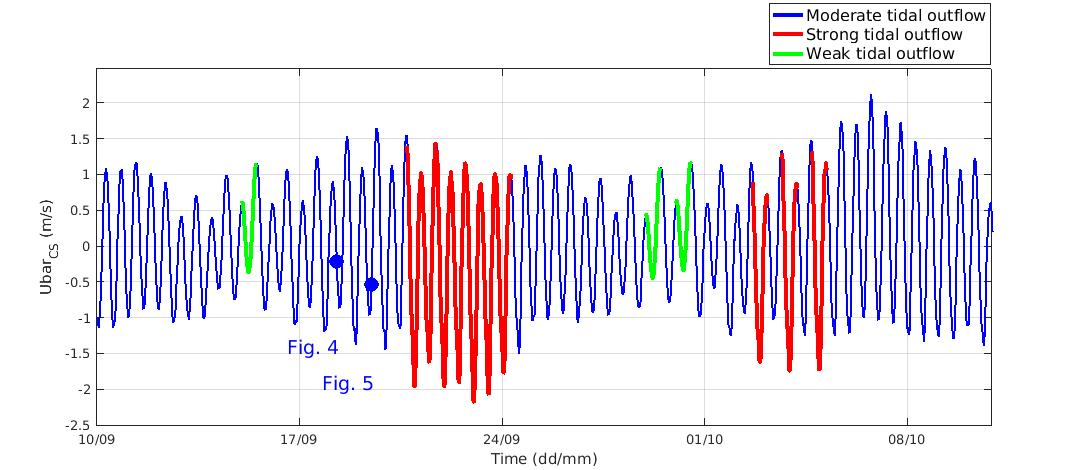
\includegraphics[width=6.3in,height=2.75in]{./media/image2.jpg}
	\end{Center}

%%%%%%%%%%%%%%%%%%%% Figure/Image No: 2 Ends here %%%%%%%%%%%%%%%%%%%%

\caption{Barotropic velocity above CS crest. The colored curves differentiate the three different tidal regimes : green curves - weak tidal forcing, blue curves - moderate tidal forcing and red curves - strong tidal forcing. The circle markers indicate the acquisition date of the high-resolution satellite images on\  figures \ref{Fig4_Lucie} and \ref{Fig5_Lucie}.}
\label{Fig2_Lucie}
\end{figure}

\subsubsection{Comparison to high-resolution satellite images}

\vspace{\baselineskip}
An effective procedure to trace the evolution of the internal or baroclinic field consists of monitoring the spatial gradient of surface velocity. The superposition of baroclinic and barotropic currents gives rise to areas of strong horizontal convergence/divergence of the flow characterized by short-scale surface roughness which can be captured by SARs [Alpers, 1985] and MSI- Multispectral Imager. This allows the identification of baroclinic structures such as internal hydraulic jumps or internal propagating internal waves through the observation of the ocean surface. \par


\vspace{\baselineskip}
Multiple SAR and RGB images have been acquired from Sentinel-1 and Sentinel-2 satellites during the modelled time period (10/09/2017 - 10/10/2017). We focus on two particular satellite images acquired both in moderate regime but at different phases of the tidal cycle: \par

- a SAR image acquired on the 18/09/2017 – 06:27:42\textit{\  }at the end of the tidal cycle\par

- a RGB image acquired \textit{ }the 19/09/2017 – 11:18:00 just after the tidal maximal outflow. \par


\vspace{\baselineskip}
The SAR image was taken at the end of a moderate tidal cycle when the well-known train of ISWs propagating eastward reaches the bay of Gibraltar (Figure \ref{Fig4_Lucie} - Left panel). The train of ISWs on the SAR image is composed at least of 4 distinct solitary waves. On this particular SAR image, a second feature is identifiable as a westward propagating internal wave in Tangier Bassin. The origin of these westward propagating internal waves will be discuss in section 2.4.3.\par

\vspace{\baselineskip}
In R\textsubscript{NBQ}, the train is composed solely of one or two solitary waves (figure \ref{Fig4_Lucie} - Right) however it reaches the bay of Gilbratar at approximately the same moment. Hence, even if the number of solitary waves in the train is underestimated in R\textsubscript{NBQ}, the propagation speed of the train seems to be well represented. Moreover, the westward propagating internal wave observed in Tangier Bassin are also quite well represented in R\textsubscript{NBQ} (location, orientation, shape). The resolution of the SAR image is 10 m, compared with a resolution of 220 m for R\textsubscript{NBQ}. The resolution of R\textsubscript{NBQ} seems therefore insufficient to represent explicitly the smallest solitary waves of the train. 
\par

%%%%%%%%%%%%%%%%%%%% Figure/Image No: 3 starts here %%%%%%%%%%%%%%%%%%%%

\begin{figure}[!h]
	\begin{Center}
		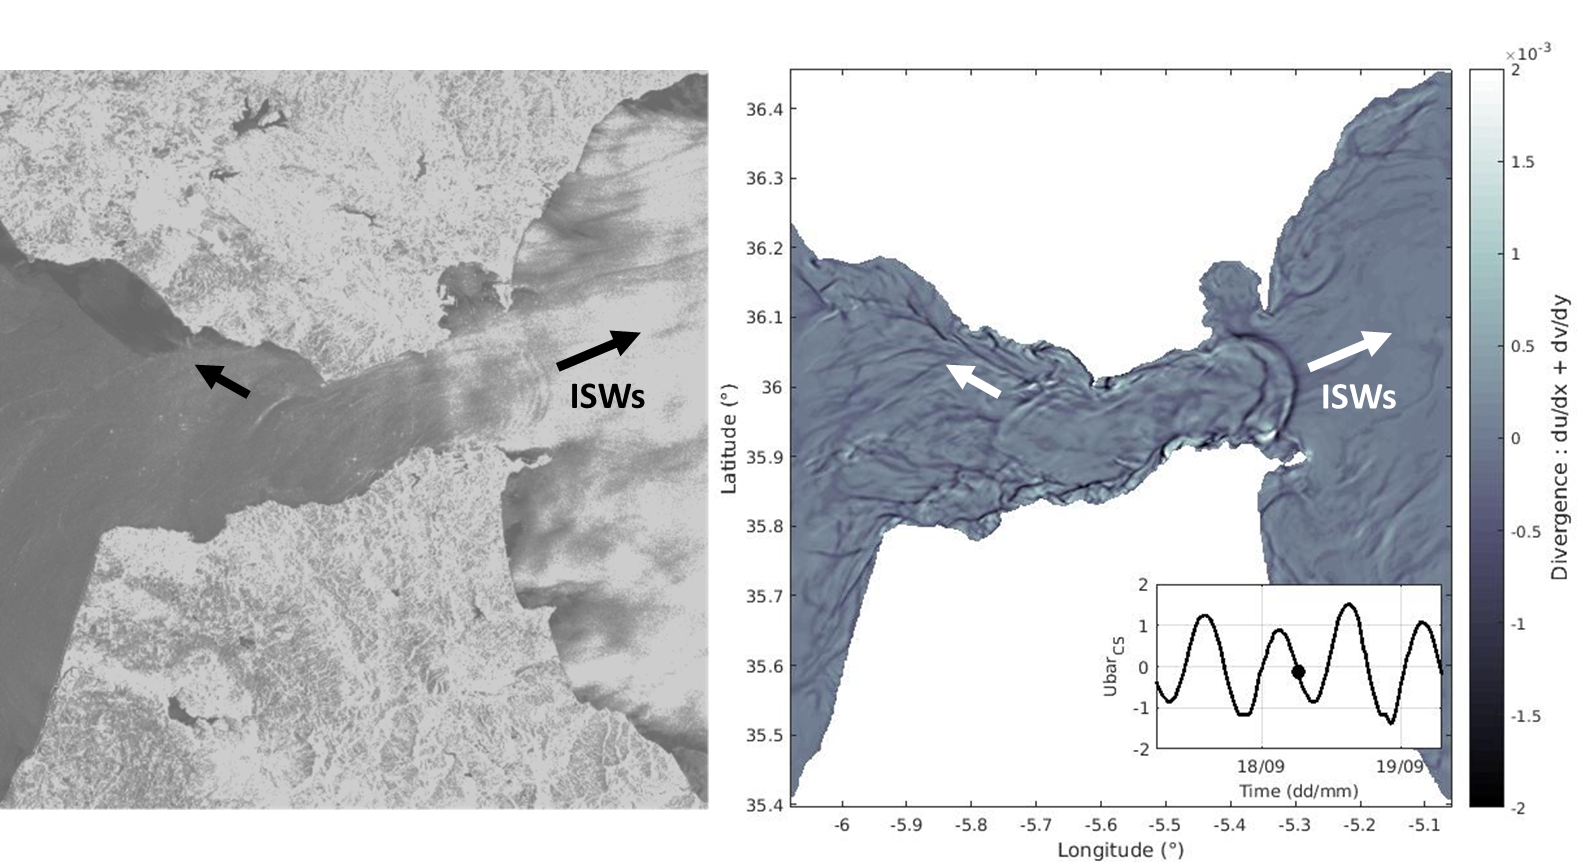
\includegraphics[width=6.3in,height=3.43in]{./media/image3.png}
	\end{Center}

%%%%%%%%%%%%%%%%%%%% Figure/Image No: 3 Ends here %%%%%%%%%%%%%%%%%%%%

\caption{Left – Sentinel-1 Synthetic Aperture Radar (SAR) image acquired on the 18/09/2017 – 06:27:42 and processed by ESA. Right - Divergence of the surface velocity in R\textsubscript{NBQ} the 18/09/2017 – 06:25:00 after a moderate tidal outflow. }
\label{Fig3_Lucie}
\end{figure}

\vspace{\baselineskip}
The RGB image (Figure \ref{Fig5_Lucie} - Left panel) was taken just after the maximum of a moderate tidal outflow when hydraulic jumps are presumably formed in the lee-side of the main sill. On this particular RGB image, instead of the expected single wavefront, two distinct fronts can be observed in CS area : one downstream of CS extending all across the strait and another one located upstream of CS and of smaller extension. At this stage of the tidal cycle, the train of ISWs generated during the previous tidal outflow is still propagating eastward inside the Alboran sea and is made of a larger number of solitary waves than in the above SAR image.\par

\vspace{\baselineskip}
In R\textsubscript{NBQ} (Figure \ref{Fig5_Lucie} - Right), the train of ISWs propagating in the Alboran sea is composed of three solitary waves (still less than on the RGB image). Its propagation speed seems to be well represented, whereas the front deformation is slightly different. 
In R\textsubscript{NBQ}, the two distinct wave fronts observed above CS on the RGB image are located a little further west. At this time in R\textsubscript{NBQ}, the tidal current above CS turned sub-critical and the hydraulic jumps formed above CS have already been released leading to an eastward propagation of the two wave fronts. In so far as some barotropic components (such as N2) are not taken into account in R\textsubscript{NBQ}, it seems that the tidal current above CS is slightly underestimated in R\textsubscript{NBQ}.

\vspace{\baselineskip}


%%%%%%%%%%%%%%%%%%%% Figure/Image No: 4 starts here %%%%%%%%%%%%%%%%%%%%

\begin{figure}[!h]
	\begin{Center}
		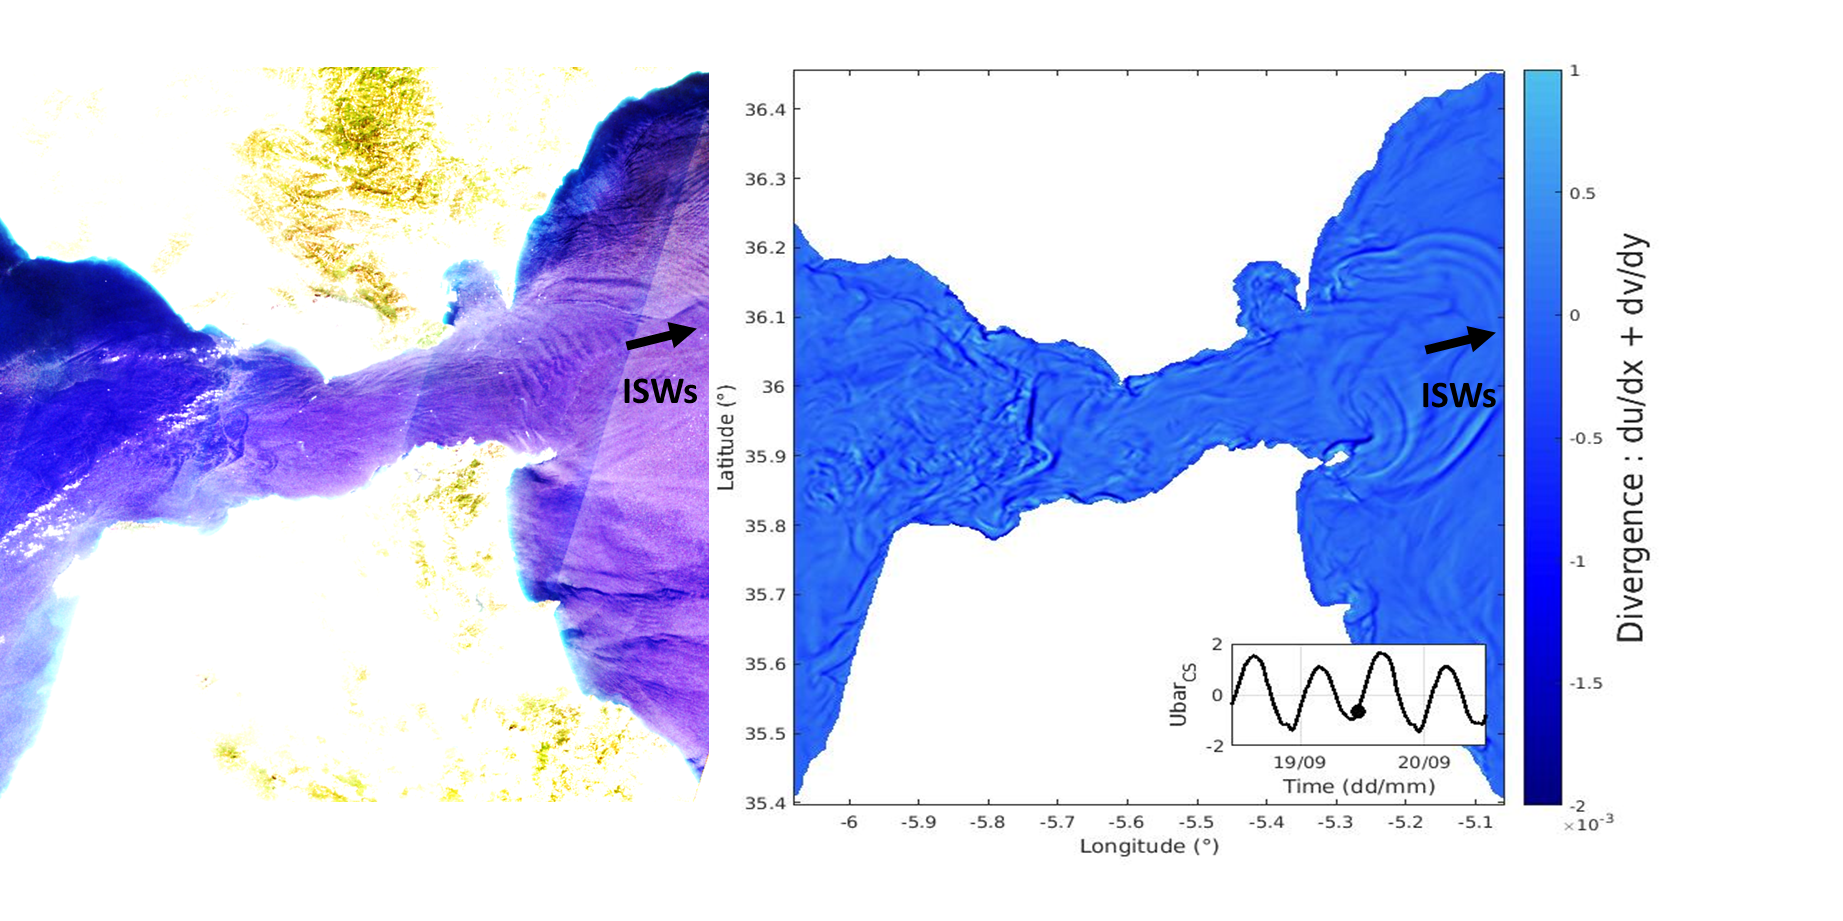
\includegraphics[width=6.3in,height=3.22in]{./media/image4.png}
	\end{Center}

%%%%%%%%%%%%%%%%%%%% Figure/Image No: 4 Ends here %%%%%%%%%%%%%%%%%%%%

\caption{Left - BOA reflectance image (RGB composites) on 19/09/2017 11:18:08, re-processed from Level-2A product for Sentinel-2A/MSI instrument distributed by ESA – Right -  Divergence of the surface velocity in R\textsubscript{NBQ}, the 19/09/2017 – 11:18:00 at a moderate tidal outflow. }
\label{Fig4_Lucie}
\end{figure}

\vspace{\baselineskip}
\subsubsection{Dynamics of the hydraulic jumps}

%%%%%%%%%%%%%%%%%%%% Figure/Image No: 5 starts here %%%%%%%%%%%%%%%%%%%%

\begin{figure}[!h]
	\begin{Center}
		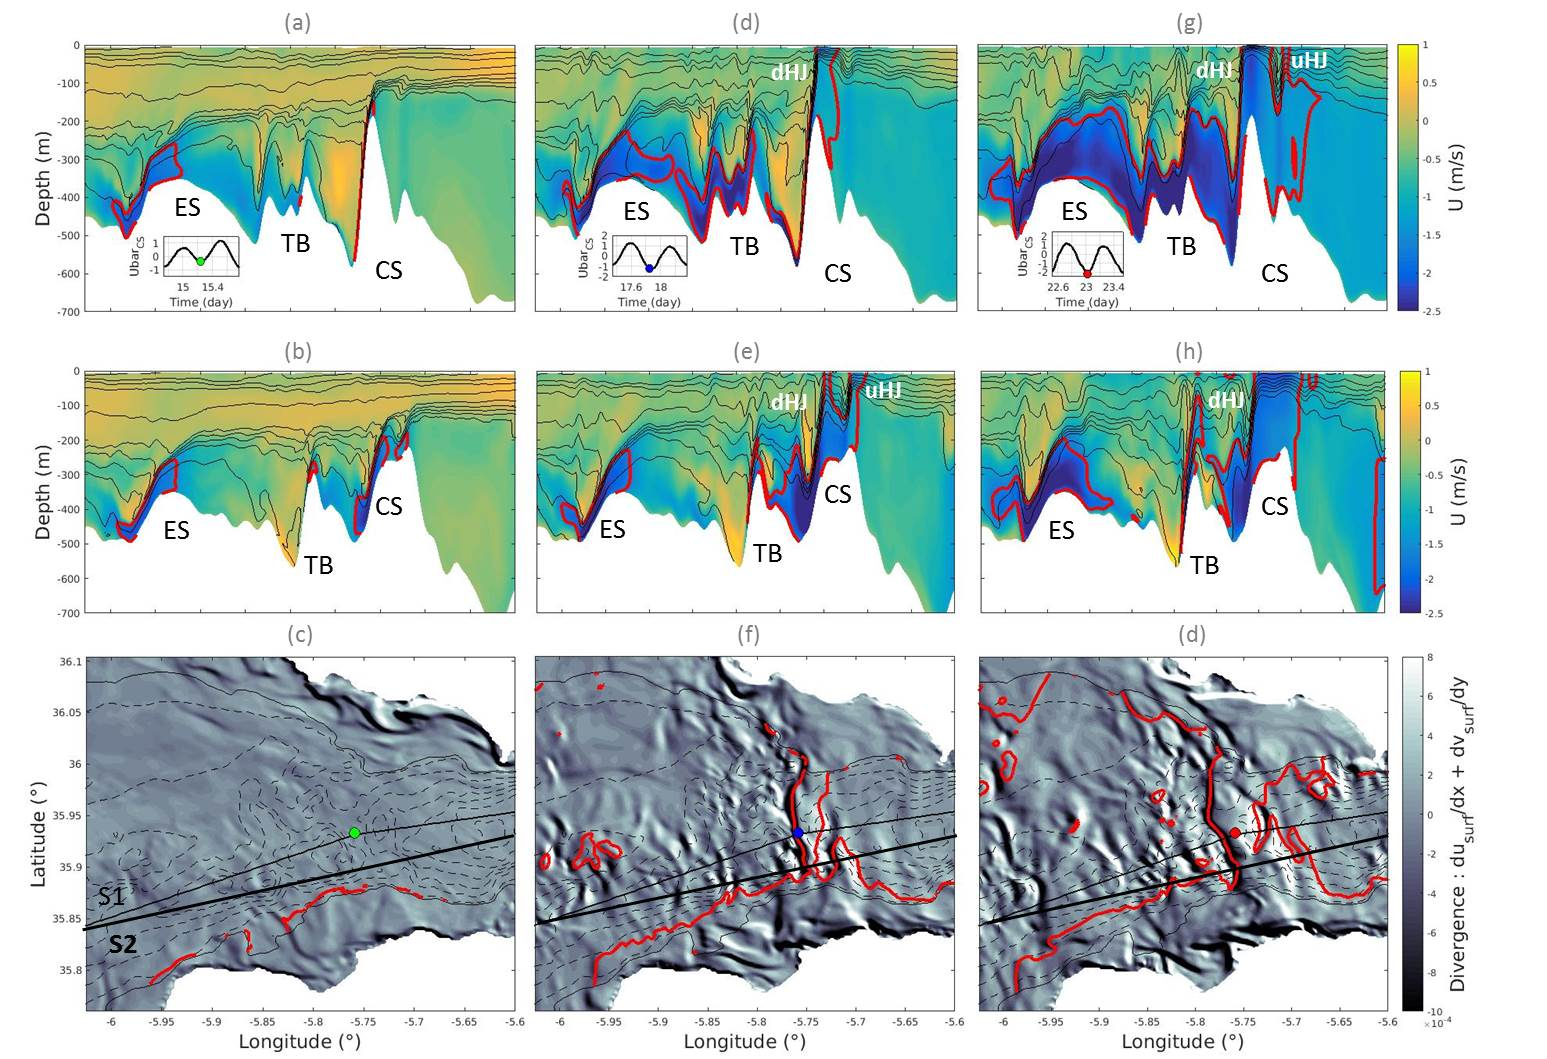
\includegraphics[width=6.61in,height=4.99in]{./media/image5.jpg}
	\end{Center}

%%%%%%%%%%%%%%%%%%%% Figure/Image No: 5 Ends here %%%%%%%%%%%%%%%%%%%%


\caption{ Lower pannels\ -  Divergence of the flow in \textbf{R\textsubscript{NBQ}} at the maximum of a weak tidal outflow (c), a moderate tidal outflow (f) and a strong tidal outflow (d). The black line locates the vertical section 1 (S1) and section 2 (S2). Middle pannels - Section 2 (S2) of the horizontal velocity field in \textbf{R\textsubscript{NBQ}} at the maximum of a weak tidal outflow (b), a moderate tidal outflow (e) and a strong tidal outflow (h). Upper pannels - Section 1 (S1) of the horizontal velocity field in \textbf{R\textsubscript{NBQ}} at the maximum of a weak tidal outflow (a), a moderate tidal outflow (d) and a strong tidal outflow (g). Red contour represent super-critical flow area (F1=c1).}
\label{Fig5_Lucie}
\end{figure}

\vspace{\baselineskip}
Under weak tidal forcing, only a small part of the bottom layer is super-critical above CS crest (partial hydraulic control figure \ref{Fig5_Lucie}.a-b). The surface layer remains sub-critical and there is no signature of any hydraulic jumps at the ocean surface (figure \ref{Fig5_Lucie}.c). \par

\vspace{\baselineskip}
Under moderate tidal forcing (figure \ref{Fig5_Lucie}.d-e), the whole water column is super-critical above CS (total hydraulic control) leading to the formation of large hydraulic jumps. The signature of these hydraulic jumps is visible on the divergence of the surface flow (figure \ref{Fig5_Lucie}.f). We can indeed observe a strong asymmetry between the northern and southern parts of the strait (due to geographical constriction) :\par

\begin{itemize}
	\item in the northern part (figure \ref{Fig5_Lucie}.d), we observe a single super-critical area above CS,\par

	\item in the southern part (figure \ref{Fig5_Lucie}.c), we observe two distinct super-critical regions above CS.
\end{itemize}\par

Hence a moderate tidal outflow is characterized by the formation of two hydraulic jumps: one located downstream of CS extending all across the strait and one located upstream of CS and confined to the southern half section of the strait\par

\vspace{\baselineskip}
Under strong tidal forcing (spring tides), when the outflow is maximal, the southern upstream hydraulic jump (located initially around\  -5.73$ ^{\circ} $ \ of longitude) is swept down to the lee side of the sill (around  -5.76$ ^{\circ} $  of longitude), and in the southern part of the strait, the flow acquires the hydraulic configuration of a pure approach-controlled state, with only one supercritical region extending from the upstream control section to a few hundred meters downstream (of CS).\par

\vspace{\baselineskip}
\subsubsection{ ISWs formation: a strong neap-spring tide variability}

\vspace{\baselineskip}
 During moderate tides (figure \ref{Fig7_Lucie}.b-e), in the middle part of the strait (section 1), an internal hydraulic jump is formed on the downstream side of CS at maximum tidal ouflow. When the tidal flow reverses, the hydraulic jump is released and leads to the eastward propagation of an internal bore (IB). It is then subject to multiple reflections (rW) in Tarrifa Narrows and degenerates into solitary waves (ISWs).\par

\vspace{\baselineskip}
However, during weak neap-tides (figure \ref{Fig7_Lucie}.a-d); the favorable hydraulic conditions for the generation of lee waves (LWs) in the lee-side of CS inhibit the internal bore generation.  \par


\vspace{\baselineskip}
During spring tides (figure \ref{Fig7_Lucie}.c-f), in the middle part of the strait, two internal hydraulic jumps are formed above CS: one upstream (uHJ) and another downstream (dHJ) of the sill. When the tidal flow reverses, the hydraulic jumps are released and lead to the eastward propagation of two internal bores (IB). The largest internal bore (emitted on the downstream side) propagates faster and catches up the smallest one (emitted on the upstream side). It is then subject to multiple reflections (rW) in Tarrifa Narrows and degenerates into solitary waves (ISWs).\par

\vspace{\baselineskip}

\vspace{\baselineskip}

\vspace{\baselineskip}


%%%%%%%%%%%%%%%%%%%% Figure/Image No: 6 starts here %%%%%%%%%%%%%%%%%%%%

\begin{figure}[!h]
	\begin{Center}
		\includegraphics[width=6.3in,height=4.32in]{./media/image6.jpg}
	\end{Center}

%%%%%%%%%%%%%%%%%%%% Figure/Image No: 6 Ends here %%%%%%%%%%%%%%%%%%%%

\caption{ Upper panels \textbf{- }Section 1 of the density field in \textbf{R\textsubscript{NBQ}} after a weak tidal outflow (a), a moderate tidal outflow (b) and a strong tidal outflow (c). Lower panels - Space-time diagram of the vertical isopycnal displacement for $ \rho $ =1031.1 kg/m3 (bold black line on the upper panels) along the section 1 during two weak tidal cycle (a), a moderate and a weak tidal cycle (b) and two strong tidal cycle (c). The white arrows represent the mean tidal inflow above Camarinal sill whereas colored arrows represent the mean tidal outflow above Camarinal sill (green for weak, blue for moderate and red for strong). Horizontal black lines locate temporally the vertical section of the density field (upper panels) whereas colored dotted\ lines locate temporally the maximum of the previous tidal outflow (section 1 on Fig.  \ref{Fig5_Lucie}). }
\label{Fig7_Lucie}
\end{figure}

%\vspace{\baselineskip}

%\printbibliography
%\end{document}

 
\selectlanguage{french}


%%%%%%%%%%%%%%%%%%%%%%%%%%%%%%%%%%%%%%%%%%%%%%%%%%%%%%%%%%%%%%%%%%%
%%%%%%%%%%%%%%%%%%%%%%%%%%%%%%%%%%%%%%%%%%%%%%%%%%%%%%%%%%%%%%%%%%%
%%% Maquette 3D NH-HR
%%%%%%%%%%%%%%%%%%%%%%%%%%%%%%%%%%%%%%%%%%%%%%%%%%%%%%%%%%%%%%%%%%%
%%%%%%%%%%%%%%%%%%%%%%%%%%%%%%%%%%%%%%%%%%%%%%%%%%%%%%%%%%%%%%%%%%%
\newpage
\null
\newpage
\section{Maquette 3D NH-HR \textit{(Tâche 1.2)}}
\label{section3DNHNR}

\noindent\fbox{\noindent\begin{minipage}{1\textwidth}
\noindent La maquette tri-dimensionnelle NH-HR est la maquette la mieux résolue sur l'horizontale (45 m) et la verticale (40 niveaux $\sigma$) implémentée dans le cadre du présent contrat.  De façon originale, cette maquette permet la simulation des "grandes structures turbulentes" \textit{(LES)}. Elle est pour cela basée sur le coeur non-hydrostatique et non-Boussinesq CROCO et met en oeuvre les schémas d'advection d'ordre supérieur et les schémas de diffusion turbulente isotropes disponibles dans CROCO, trois éléments essentiels et indispensables pour simuler numériquement à minima les instabilités primaires amorçant la cascade turbulente directe. Une comparaison détaillée de la dynamique à haute résolution avec celle simulée avec la maquette à plus basse résolution (NH-REF, section \ref{section3DNHREF}) montre que les processus de grande échelle sont représentés de façon comparable dans les deux maquettes. La simulation NH-HR permet en outre un raffinement du train d'ondes solitaires et surtout une représentation cohérente et explicite des instabilités de Kelvin-Helmholtz générées au voisinage du jet méditerranéen. 
\end{minipage}
}

\subsection{Caractéristiques de la maquette NH-HR}

Les caractéristiques numériques de la maquette à plus haute résolution NH-HR sont présentées dans le tableau \ref{tab_XEC}. Cette maquette est environ 4 fois mieux résolue que la maquette à basse résolution NH-REF dans chacune des deux directions horizontales (45 m contre 220 m) et la résolution verticale reste la même  (40 niveaux verticaux de type $\sigma$). Les épaisseurs minimales et maximales des couches $\sigma$ sont fournies dans cette table: la résolution verticale est la maquette est de l'ordre de la dizaine de mètre dans la région du détroit, et elle 2 fois plus grande que la résolution horizontale dans les zones les plus profondes.\\

\begin{table}[!h]
        %\begin{minipage}{.6\textwidth}
        \centering
        \begin{tabular}{|p{\linewidth/3}|c|c|}
                \hline
                Coeur numérique & \multicolumn{2}{c|} {CROCO-NBQ} \\
                Domaine & \multicolumn{2}{c|} {6°4.8'W  5°3.4'W ;}\\
                & \multicolumn{2}{c|} {35°23.8'N  36°27.4'N}\\
                Nombre de points de grille horizontaux & \multicolumn{2}{c|} {2049x2621}  \\
                Nombre de niveaux verticaux ($\sigma$) & \multicolumn{2}{c|} {40} \\
                %\hline
                $\Delta x = \Delta y$ & \multicolumn{2}{c|} {45 m}\\
                %\hline
                Depth & Min & Max\\
                %\cline{2-3}
                & 26 m & 960 m\\
                %   \hline
                $\Delta$z & 0.7 m & 24 m\\
                Nombre de coeurs & \multicolumn{2}{c|} {447 (+1 serveur xios)}\\
                Pas de temps interne ($\Delta t_s$) & \multicolumn{2}{c|} {1 s}\\
                Pas de temps externe ($\Delta t_f$) & \multicolumn{2}{c|} {1/11 s}\\
                Schémas d'advection & \multicolumn{2}{c|} {WENO-5 (T-S) , TVD (U-V-W)} \\
                Coefficient de viscosité verticale $\nu$ & \multicolumn{2}{c|} {10$^{-6}$ m^{2}/s} \\
                Coefficient de mélange vertical $K_\rho$ & \multicolumn{2}{c|} {10$^{-6}$ m^2/s}\\
                $C_s$ & \multicolumn{2}{c|} {400 m/s}\\
                Ondes de marée & \multicolumn{2}{c|} { $\text{M}_{\text{2}}$, $\text{S}_{\text{2}}$,                            $\text{K}_{\text{1}}$, $\text{O}_{\text{1}}$ }\\
                \hline
        \end{tabular}
        \captionof{table}{Principales caractéristiques de la maquette NH-HR.}
        \label{tab_NH-HR}
        %\end{minipage}
\end{table}

L'hydrologie, les courants de marée et la circulation générale sont forcés comme pour la maquette NH-REF à partir d'une simulation hydrostatique "Mère" MitGcm du modèle opérationnel de la Méditerranée et de la Mer Noir de l'ENEA, gracieusement fournie par l'équipe de G. Sannino (ENEA, Rome)\footnote{http://www.enea.it/it/seguici/pubblicazioni/pdf-volumi/cresco-report-2016.pdf}. Ce forçage est utilisé comme condition initiale et comme conditions aux frontières ouvertes. Cette simulation "Mère" a une résolution horizontale variable d'environ 700 m dans la région du détroit, soit environ une quinzaine de fois supérieure à celle de la maquette à haute résolution NH-HR. Ce saut en résolution relativement élevé est associé à un changement de coordonnées verticales (le MitGcm est basé sur une grille à niveaux z, CROCO sur une grille $\sigma$).  Les cœurs dynamiques utilisés dans les simulations "Mère" et NH-HR sont de plus différents: la maquette NH-HR est en effet non-hydrostatique et non-Boussinesq alors que la version du modèle MitGcm utilisée pour réaliser la simulation "Mère" est hydrostatique et Boussinesq.\\
L'ensemble de ces différences est à l'origine d'un choc violent lorsque la simulation NH-HR est initialisée et forcée directement à partir de la simulation Mère MitGcm. Un tel choc entraîne une période de \textit{spin-up} de plusieurs heures durant lesquelles la qualité des caractéristiques des masses d'eaux méditerranéenne et atlantique est peut-être fortement dégradée. En conséquence, un protocole de simulation spécifique a été mis en place:
\begin{itemize}
	\item La simulation à haute résolution (HR) est initialisée et forcée par la simulation "Mère" MitGcm.
	\item Durant les 6 premières heures de simulation, le coeur hydrostatique, Boussinesq de CROCO est implémenté, limitant ainsi le choc initial et permettant une première "mise en équilibre" des champs initiaux sur la bathymétrie à haute résolution.
	\item La simulation HR est alors redémarrée (\textit{Hot Restart}) en version non-Hydrostatique et non-Boussinesq.
\end{itemize}
Quatre ondes de marées sont forcées aux frontières latérales: ($\text{M}_{\text{2}}$, $\text{S}_{\text{2}}$, $\text{K}_{\text{1}}$, $\text{O}_{\text{1}}$). Ce forçage est intégré dans les sorties issues de la simulation MitGcm à 700 m.\\

\subsection{Évaluation des coûts de calcul}

 La résolution et l'extension horizontale de la maquette NH-HR sont choisies de telle sorte que les structures dynamiques les plus fines possibles puissent être explicitement simulées dans la région du détroit de Gibraltar pour un coût de calcul "raisonnable" avec le coeur non-hydrostatique et non-Boussinesq de CROCO. Le coût relatif de calcul de la maquette NH-HR est d'environ 0.8 (0.8 heures de calcul pour 1 heure simulée sur 447 cœurs sur la machine Datarmor). Le sur-coût associé au coeur non-hydrostatique et non-Boussinesq est d'environ 3 par rapport au coeur hydrostatique CROCO.\\
Ce ratio de 0.8 autorise la simulation de plusieurs périodes de marée semi-diurne et permet par conséquent l'étude détaillée du contrôle hydraulique, de la génération d'instabilités primaires et d'ondes de gravité internes de grande amplitude dans la région du détroit. Une analyse harmonique plus fine des principales composantes de marée nécessiterait toutefois une simulation de plus longue durée.

\subsection{Évaluation de la qualité des principales ondes de marée simulées}
La qualité des ondes de marée simulées dans la simulation NH-HR est évaluée en deux temps:
\begin{itemize}
	\item Une inter-comparaison des anomalies de surface simulées dans les maquettes NH-REF et NH-HR a été réalisée sur l'ensemble du domaine numérique. L'erreur quadratique moyenne est d'environ 5 cm entre les deux maquettes, avec des valeurs plus élevées à l'est et au nord. 
	\item Deux marégraphes disponibles dans la région simulée sont utilisés pour évaluer les erreurs l'élévation du niveau de la mer. Les résultats de cette évaluation sont détaillés au chapitre \ref{chapitredelivrables}, section \ref{mareedelivrable} du présent rapport.
\end{itemize}

\subsection{Ressaut hydraulique}

La maquette NH-HR simule correctement le contrôle hydraulique localisé dans la région du seuil de Camarinal. Un tel contrôle est attendu dans cette région lorsque les courants de marée sont suffisamment puissants pour que le flot au-dessus du seuil devienne supercritique. Ce processus intervient à chaque période de marée durant 3 à 4 heures lorsque les courants de marée sont orientés vers l'Atlantique Nord (à l'exception notable de certaines périodes en régime de mortes-eaux durant lesquelles ces courants sont trop faibles). Le contrôle entraîne la formation d'un ressaut hydraulique dont la géométrie va dépendre de l'intensité des courants de marée. \\
La figure \ref{fig_ressaut_NH-HR}.a présente une coupe verticale dans la région du Seuil de Camarinal lors d'une période d'\textit{outflow} maximum simulée avec la maquette NH-HR, et la figure \ref{fig_ressaut_NH-HR}.b la trace visible du ressaut en terme d'élévation de la surface libre dans la simulation. Le ressaut est visible sur la coupe vers -5.755° longitude dans la région où les surfaces isopycnales présentent une discontinuité d'une amplitude d'environ 70 m au-dessus du seuil.\\

\subsection{Instabilités primaires (\textit{LES})}

Dans la zone du jet méditerranéen sur le flanc ouest du seuil de Camarinal, la maquette NH-HR montre l'apparition d'instabilités primaires de type Kelvin-Helmholtz, telles qu'elles ont pu être observées par Wesson and Gregg (1994). Ces instabilités n'étaient pas présentes dans la simulation plus basse résolution (220 m) réalisée à partir de la maquette NH-REF. La présence potentielle de telles instabilités est confirmée par le calcul du nombre de Richardson, inférieur à 1/4 dans la région du ressaut. La faiblesse du nombre de Richardson s'explique par le fort cisaillement entre le jet Méditerranéen (vitesse supérieure à 2 m/s) et l'écoulement des eaux Atlantiques (de l'ordre de quelques dizaines de centimètres par seconde).\\
La figure \ref{Coupe_Melange} prolonge la coupe de la figure \ref{fig_ressaut_NH-HR} dans le Bassin de Tanger et au-dessus du Seuil d'Espartel, et montre une comparaison du champs de masse volumique dans la maquette à haute résolution NH-HR et dans la maquette NH-REF.\\
Une différence importante est l'augmentation notable de l'épaisseur du jet méditerranéen dans la simulation à haute résolution en aval (pour le jet méditerranéen) de chacun des accidents bathymétriques présents dans cette section verticale. La remontée des surfaces isopycnales observée sur cette figure pour la simulation à haute résolution peut sembler paradoxale puisque, pour des contraintes bathymétriques quasi-équivalentes, une augmentation de la seule résolution horizontale devrait plutôt conduire à une représentation plus fine du jet méditerranéen. Une explication pourrait être apportée par la présence de nombreuses instabilités de type Kelvin-Helmholtz se développant dans cette région. Ces instabilités primaires amorcent la cascade turbulente directe et entraînent un brassage \textit{(stirring)} explicitement simulé avec une résolution de 45 m. Ce brassage est finalement lui-même à l'origine d'une augmentation du mélange. Dans la simulation à plus basse résolution, ces instabilités constituent des processus "sous-maille", mal résolus pour lesquels un schéma de turbulence plus adapté devrait être mis en place. Ces résultats très préliminaires doivent maintenant être confirmés et de nouveaux diagnostiques sont en cours d'implémentation afin, en particulier, de mieux comprendre l'impact de la simulation des grandes structures turbulentes sur le mélange.\\


\begin{figure}[!h]
        \includegraphics[width=\textwidth]{./ressaut_2D_it790_vhr_IE2.png}
        \caption{a) Coupe verticale du seuil de Camarinal. Couleur : vorticité d'axe y, traits plein : isopycnes, et vecteurs vitesse u-w. b) Élévation de la surface libre simulée avec la maquette NH-HR}
        \label{fig_ressaut_NH-HR}
        \end{figure}

\begin{figure}[!h]
        \includegraphics[width=\textwidth]{./media/comp_GExO_hr-vhr_IE.png}
        \caption{Coupe verticale selon la section S2 de la figure \ref{fig_mod1_HR-REF}.b de la masse volumique dans les 2 maquettes 3D en $kg.m^{-3}$. En couleur: simulation NH-HR (résolution dec45 m, 40 niveaux $\sigma$), contours pointillés: simulation NH-REF (résolution de 220 m, même nombre de niveaux $\sigma$).}
        \label{Coupe_Melange}
        \end{figure}
  	
\subsection{Ondes internes de grande amplitude}

Comme son homologue à plus basse résolution NH-REF, la maquette à haute résolution NH-HR est permet de simuler la génération et la propagation des modes 1 et 2 d'ondes internes de gravité dans le détroit de Gibraltar, ce qui est en accord avec les observations des satellites Sentinel 1 et 2. De façon similaires, des ondes de grande amplitude (de l'ordre de la centaine de mètres), sont générées lors de la relaxation du ressaut hydraulique au Seuil de Camarinal. Ces ondes ont une signature de mode 1. Elles sont précédées par la propagation d'un mascaret interne puis se décomposent en train d'ondes solitaires sous l'action de la dispersion non-hydrostatique qui vient équilibrer les non-linéarités liées à l'advection. Au cours de sa propagation dans le détroit de Tarifa, ce train d'onde va en partie se réfléchir sur les côtes en train ondes se propageant vers l'ouest. Afin de détailler l'apport de l'augmentation de la résolution sur ces ondes, la figure \ref{fig_mod1_HR-REF}.a présente une coupe verticale en densité du train d'ondes solitaires alors qu'il entre en Mer d'Alboran dans la maquette NH-HR (en couleur) et dans la maquette NH-REF (en pointillés). \\
Les ondes de mode 1 se sont propagées plus vite dans la maquette NH-HR, et le nombre d'ondes dans le train est plus grand (5 contre 2). Ce comportement est le même à chaque période de marée et la variation du nombre de solitons d'une période de marée à une autre peut être simulée avec la maquette NH-HR. Cette forte variabilité diurne est illustrée dans le tableau \ref{tab_XEC}, réalisé en notant l'arrivée de l'onde de mode 1 au point le plus à l'est dans la figure \ref{fig_mod1_HR-REF}.a (ou à tous les points de la figure \ref{fig_mod1_HR-REF}.b pour le calcul de la vitesse de propagation). Les vitesses les plus fortes dans ce tableau correspondent à une advection par des courants de marée plus importants, on observe que ces périodes sont associées à un plus petit nombre d'ondes dans le train avec une périodicité elle aussi plus petite. Il est à noter que ces valeurs ne sont pas identiques pour toutes les latitudes à la sortie du détroit: du fait de la dispersion induite par la force de Coriolis, l'amplitude de la première onde est par exemple plus grande dans la partie sud.

\begin{figure}[!h]
 	\includegraphics[width=\textwidth]{media/comp_train_it36_IE2_hr-vhr.png}
 	\caption{a) Coupe verticale selon la section S1 de densité (kg/m$^3$) dans les maquettes NH-REF (pointillés) et NH-HR (couleurs). b) Surface libre simulée avec la maquette NH-HR avec trace des sections S1 et S2 et points ayant servis pour la table \ref{tab_XEC}.}
 	\label{fig_mod1_HR-REF}
\end{figure}

\begin{table}[!h]
	%\begin{minipage}{.6\textwidth}
	\centering
	\begin{tabular}{|l|c|c|c|c|}
		\hline
		Numéro du train &  1 & 2 & 3 & 4  \\
		\hline
		Temps écoulé depuis le passage du train précédent (jour) & & 0.42 &0.6 & 0.41\\
		Vitesse dans le détroit de Tarifa (m/s) & 1.6 & 1.9 & 1.6 & 2.1\\
		Nombre d'ondes constituant le train & 11 & 5 & 8 & 2 \\
		Amplitude du premier soliton (m) & 50 &70 &45 &40\\
		Période moyenne (mn) & 20 & 12 & 18 & 12.5\\
		\hline
	\end{tabular}
	\captionof{table}{Caractéristiques train d'ISW sortie est du détroit pour conditions MM}
	\label{tab_XEC}
	%\end{minipage}
\end{table}

\subsection{Génération de tourbillons dans le sillage des solitons}

Les simulations NH-REF et NH-HR montrent la génération d'un tourbillon au passage des trains de solitons à la sortie du détroit. Cette génération pourrait être une conséquence des violents cisaillements de courants horizontaux générés par l'onde interne.\\
La structure tourbillonnaire demeure dans cette région puis déforme le train d'ondes solitaires suivant. A notre connaissance, il n'existe pas d'observations ni de preuves directes de son existence.\\
Son impact sur les solitons n'est toutefois pas négligeable puisque les simulations numériques montrent pour certaines périodes de marées une désorganisation du train d'ondes solitaires à la sortie du détroit. Cette déstructuration du train d'ondes solitaires pourrait être une conséquence de son interaction avec le tourbillon suivant ou être associée à la génération de la structure tourbillonnaire. Ces conséquences ont été observées par (Vlasenko et al., 2009) et pourraient quoiqu'il en soit confirmer indirectement la présence de la structure tourbillonnaire. Il convient toutefois d'être prudent et de nouvelles investigations sont actuellement en cours afin de préciser le mécanisme de génération du tourbillon et de rassembler des observations in situ pouvant confirmer sa présence.

\subsection{Sensibilité au protocole de simulation et évolution de la maquette}
La maquette NH-HR n'est bien sûr pas figée et plusieurs évolutions sont actuellement en cours:
\begin{itemize}
 \item La bathymétrie utilisée dans la maquette NH-HR du présent rapport est celle de la grille HOMONIM résolue à 500 m. Une bathymétrie résolue à 100 m du détroit a plus récemment été fournie et est en cours d'implémentation et de test dans la simulation NH-HR.
 \item La maquette NH-HR a été utilisée pour simuler la dynamique du détroit dans différents régimes de marées (mortes-eaux, vives-eaux et marée moyenne), présentés au chapitre \ref{chapitredelivrables}. Leur exploitation est actuellement en cours.
 \item L'impact de la stratification et de son évolution saisonnière sera explorée prochainement en choisissant une initialisation à une date différente dans les champs fournis par l'ENEA. Cette étude sera toutefois associée au retour du forçage atmosphérique afin de simuler de la façon la plus réaliste possible les mécanismes locaux de re-stratification. Comme indiqué en introduction du présent rapport, le groupe CROCO-Aérologie a en effet souhaité aborder par étapes l'étude de la dynamique dans la région du détroit. Lorsque cela a un sens, les forçages et par conséquent les processus et autres mécanismes physiques sont introduits progressivement. L'objectif d'une telle approche est double: mieux comprendre la dynamique locale et mieux contrôler le protocole de modélisation numérique.
\end{itemize}

\subsection{Discussion, conclusions}

La maquette NH-HR permet, de façon attendue, de raffiner la simulation des ondes solitaires se propageant en direction de la Méditerranée depuis le détroit de Gibraltar. Une étude plus détaillée de ces ondes de grande amplitude à partir d'observations dédiées et, ou, d'une modélisation simultanée avec un modèle simplifié de type KdV devrait fournir de précieuses informations sur l'impact de la résolution sur la dissipation physique et la dissipation numérique, sur la dispersion non-hydrostatique ou encore sur la bonne représentation des processus non-linéaires.\\
La maquette  NH-HR autorise en outre de façon originale la simulation explicite des "grandes structures turbulentes" (simulation dite \textit{LES}) dans la région du détroit de Gibraltar. L'augmentation de la résolution entre les maquettes NH-REF et NH-HR autorise en effet la simulation des structures tourbillonnaires associées aux instabilités primaires de type Kelvin-Helmholtz entre les masses d'eaux méditerranéenne et atlantique. Ces instabilités marquent classiquement l'amorce de la cascade turbulente directe induisant localement un important mélange des masses d'eaux. Ces instabilités ne sont pas représentées dans la simulation NH-REF par manque de résolution effective. Elles ne pourraient être simulées explicitement dans une simulation hydrostatique de même résolution (45 m) dans cette région. Ces instabilités sont en effet associées à une vorticité relative d'axe horizontal qui ne peut être simulée sous une hypothèse hydrostatique. Un résultat important pour cette première simulation pouvant être qualifiée de \textit{LES} concerne les différences importantes entre le mélange simulé au moyen des maquettes NH-REF et NH-HR. L'intercomparaison montre à minima une très forte dépendance au protocole de simulation. La maquette NH-REF (de type \textit{RANS}\footnote{RANS: Reynolds Average Navier Stokes simulation, simulation basée sur une représentation implicite des "grandes structures turbulentes" à partir d'un schéma de fermeture turbulent.}) permet une simulation implicite du mélange et dépend pour cela entièrement du schéma de fermeture turbulente.\\
La maquette NH-HR montre donc l'importance d'une représentation explicite des "grandes structures turbulentes" dans des régions dynamiquement instables telles que la région du ressaut hydraulique. Elle donne de plus l'ordre de grandeur de la résolution horizontale (environ 45 m) et verticale (40 niveaux $\sigma$) permettant la simulation explicite des instabilités primaires.\\
Une première évaluation de la pertinence et de la qualité des structures instables simulées a pu être réalisée à partir d'observations publiées (Wesson and Gregg 1994). Un protocole d'observations dédié devra toutefois être plus spécifiquement mis en oeuvre pour espérer évaluer les caractéristiques principales de ces instabilités (localisation spatio-temporelle, amplitude...) et surtout pour quantifier les caractéristiques statiques du mélange qu'elles induisent. La campagne d'observations planifiée par le SHOM dans la région du détroit à la fin de l'été 2020 (soit un peu plus d'un an après la publication du présent rapport) devrait sans aucun doute répondre à un certain nombre de questions. Les maquettes numériques développées et évaluées dans le cadre du projet Gibraltar 16CR01 pourront être utilisées pour préparer cette campagne via par exemple la génération d'observations synthétiques.\\
Une discussion des principales perspectives associées à l'exploitation de la dynamique simulée d'une part et à l'évolution du protocole de simulation d'autre part est fournie au chapitre \ref{chapitreconclusion}.

%%%%%%%%%%%%%%%%%%%%%%%%%%%%%%%%%%%%%%%%%%%%%%%%%%%%%%%%%%%%%%%%%%%
%%%%%%%%%%%%%%%%%%%%%%%%%%%%%%%%%%%%%%%%%%%%%%%%%%%%%%%%%%%%%%%%%%%
%%% Généralisation du système de coordonnées
%%%%%%%%%%%%%%%%%%%%%%%%%%%%%%%%%%%%%%%%%%%%%%%%%%%%%%%%%%%%%%%%%%%
%%%%%%%%%%%%%%%%%%%%%%%%%%%%%%%%%%%%%%%%%%%%%%%%%%%%%%%%%%%%%%%%%%%
\newpage
\section{Généralisation du système de coordonnées verticales.\\ \textit{(Tâche 2)}}

Une pré-étude sur la pertinence d'une évolution du système de coordonnées verticales a été conduite par le professeur Eric Chassignet accueilli en 2017-2018 par le laboratoire d'Aérologie. Ce travail correspond à la Tâche 2 du contrat Gibraltar 16CR01 et a été décomposé en deux sous-tâches:
\begin{itemize}
\item{Analyse des solutions techniques \textit{(Tâche 2.1)}},
\item{Mise en œuvre et validation \textit{(Tâche 2.2)}}.
\end{itemize}
Le rapport final écrit par Eric Chassignet est fourni en Annexe.\\
Eric Chassignet a de surcroît co-organisé la première réunion des utilisateurs CROCO \textit{(CROCO USER-MEETING)} à Toulouse en Mai 2017.\\
 

%%%%%%%%%%%%%%%%%%%%%%%%%%%%%%%%%%%%%%%%%%%%%%%%%%%%%%%%%%%%%%%%%%%
%%%%%%%%%%%%%%%%%%%%%%%%%%%%%%%%%%%%%%%%%%%%%%%%%%%%%%%%%%%%%%%%%%%
%%% Chapitre Délivrables
%%%%%%%%%%%%%%%%%%%%%%%%%%%%%%%%%%%%%%%%%%%%%%%%%%%%%%%%%%%%%%%%%%%
%%%%%%%%%%%%%%%%%%%%%%%%%%%%%%%%%%%%%%%%%%%%%%%%%%%%%%%%%%%%%%%%%%%
\chapter{Délivrables, fourniture d'un \textit{produit numérique}.\\ \textit{(Tâche 3)}}

\label{chapitredelivrables}

\noindent\fbox{\noindent\begin{minipage}{1\textwidth}
Trois simulations ont été réalisées à partir de la maquette à haute résolution (45 m) NH-HR pour des marées de mortes-eaux, de vives-eaux et pour une marée d'amplitude moyenne. La dynamique des principales ondes de marée et la dynamique sub-tidale sont respectivement évaluées. 
\end{minipage}
}

\section{Protocole de simulation}
Début 2018, le contrat Gibraltar 16CR01 a fait l'objet d'un avenant portant sur la \textit{fourniture d'un produit numérique élaboré sur la base des maquettes numériques du détroit de Gibraltar telles que mises en place à la tâche 1}. Ce "produit numérique" est constitué de trois simulations numériques et leurs diagnostiques. Ces simulations numériques s'appuient sur la maquette numérique la plus réaliste et la mieux résolue présentée en section \ref{chapitremodele}.\ref{section3DNHNR}: la maquette NH-HR.
\\

\noindent Trois simulations \textit{(LES)} ont été réalisées avec la maquette NH-HR respectivement en condition de mortes-eaux (ME), vives-eaux (VE) et pour une marée intermédiaire (MM) entre ces deux marées extrêmes. 
Les dates de début et de fin de ces simulations sont données dans la table \ref{tab_dates_MIV}. 
Notons que ces périodes n'incluent pas les 6h de simulation hydrostatique nécessaires à l'initialisation (\textit{spin-up}). 
Notons également qu'il n'y a pas d'autres processus de forçage (eg. circulation grande échelle, surcotes...) que la marée imposée aux frontières du domaine.

\noindent La fréquence d'archivage des variables est de 1h sur l'ensemble du domaine, elle est moindre sur des zones d'intérêts pré-identifiées :
\begin{itemize}
\item Sur la région du Seuil de Camarinal (5°42'W - 5°48'W 35°52'N - 36°N) : sorties toutes les 2 minutes.
\item Sur l'entrée en Mer d'Alboran (5°3'W - 5°20'W 35°50'N - 36°10'N) : sorties toutes les 15 minutes.
\end{itemize}
Le forçage barotrope de marée est issu de simulations du modèle opérationnel de l'ENEA (voir section \ref{chapitremodele}.\ref{section3DNHNR}) et contient uniquement les 4 composantes de marée $M_2$, $S_2$, $K_1$ et $O_1$. 
La stratification est également issue de ce modèle aux dates d'initialisation de 
chacune des 3 situations.\\

\begin{table}[h]
        %\begin{minipage}{.6\textwidth}
        \centering
        \begin{tabular}{|c|c|}
                \hline
                Situation & Dates (UTC)\\
                \hline
                Mortes Eaux (VE) & 13/09/2017 16h00 - 15/09/17 17h00 \\
                %\hline
                Marées Moyenne (MM) & 16/09/2017 19h00 - 18/09/17 20h00  \\
                Vives Eaux (ME) & 19/09/2017 22h00 - 21/09/17 23h00  \\
                \hline
        \end{tabular}
        \captionof{table}{Périodes de simulation pour les 3 sitituations VE, MM et ME}
        \label{tab_dates_MIV}
        %\end{minipage}
\end{table}

\section{Analyse des composantes de la marée}
\label{mareedelivrable}
Les figures \ref{fig_maree_tar} et \ref{fig_maree_ceu} représentent les variations du niveau de la mer dans chaque
simulation par rapport aux données mesurées aux marégraphe de Tarifa et Ceuta. Ces données ont été mises à à disposition
gracieusement par l'institut public espagnol \textit{Puertos del Estado} et le programme \textit{GLOSS} (SHOM) \footnote{Nous remercions Puertos des Estados et le programme Gloss pour la fourniture de ces données marégraphiques. L'utilisation de ces résultats devra être également portée à leur connaissance.}.\\
Dans les 3 situations, les simulations sont en bon accord avec les observations marégraphiques. On observe toutefois de légers déphasages du cycle de marée (<1h), en avance ou au contraire en retard, selon les situations et les marégraphes. On observe aussi une différence d'amplitude entre les deux simulations et les données marégraphes résumées dans le tableau \ref{tab_rmse_MIV}. L'écart d'amplitude est de l'ordre de la dizaine de centimètres.

\begin{figure}[!h]
 	\includegraphics[width=\textwidth]{./sla_tarifa_all.png}
 	\caption{Anomalie du niveau de la mer (m) à Tarifa (36°N 5°36'W) enregistrée par le marégraphe 	(courbe noire), 
 	interpolée dans le champ de forçage (courbe rouge), dans CROCO (courbe bleu) dans la situation ME (a), MM (b) et VE (c). 
 	En tirets bleus le signal filtré à 25h dans CROCO.}
 	\label{fig_maree_tar}
\end{figure}

\begin{figure}[!h]
	\includegraphics[width=\textwidth]{./sla_ceuta_all.png}
 	\caption{Idem que figure \ref{fig_maree_tar} à Ceuta (35°54'N 5°19'W). 
 	Certaines mesures sont absentes pour la période VE.}
 	\label{fig_maree_ceu}
\end{figure}

Ces décalages ne sont pas identiques dans le cas du forçage par le MITgcm, 
soulignant la grande sensibilité de la modélisation numérique du détroit. On peut avancer comme raison à cela le fait que les bathymétries des 
2 modèles diffèrent. Les désaccords entre modèle(s) et marégraphes peuvent être dus également à un spectre de marée
incomplet voire à des processus manquants (effets de pression...). Des études complémentaires pourraient être envisagées
dans ces 2 cas. \\

\begin{table}[h]
        %\begin{minipage}{.6\textwidth}
        \centering
        \begin{tabular}{|c|c|c|c|c|}
                \hline
                Situation & \multicolumn{2}{c|}{Tarifa} &\multicolumn{2}{c|} {Ceuta}\\
                &CROCO &MitGCM&CROCO &MitGCM\\
                \hline
                Mortes Eaux (VE) &10 cm &7 cm &9 cm& 6 cm\\
                %\hline
                Marée Moyenne (MM) & 13 cm&10 cm &12 cm&9 cm \\
                Vives Eaux (ME) & 14 cm& 11 cm& 12 cm&9 cm \\
                \hline
        \end{tabular}
        \captionof{table}{Erreur quadratique moyenne de l'anomalie de niveau de la mer entre les simulations et les marégraphes.}
        \label{tab_rmse_MIV}
        %\end{minipage}
\end{table}

\section{Analyse de la dynamique aux échelles subtidales}
Le signal aux échelles subtidales est également ajouté à cette fourniture. Pour d'aussi courtes périodes de simulation (50 h), le signal de marée n'est pas filtrable par analyse harmonique 
(15 jours seraient nécessaires) ni par filtrage de Demerliac (filtre digital à 72h). Un filtrage par  moyenne glissante avec une fenêtre à 25 h a donc été implémenté et appliqué aux différentes variables (\textit{i.e.} niveau de la mer, courants, courants barotropes) issues de chaque simulation.\\
La qualité et la performance du filtrage ont été étudiées de manière statistique (écart-type temporel) en moyenne sur le domaine et aux marégraphes de Tarifa et Ceuta
où nous disposons de données sur la période étudiée. \\
En moyenne sur l'ensemble du domaine, en situation de mortes-eaux, 91\% de la variabilité du signal d'élévation du niveau de la mer est retiré par ce filtrage. 
En situation de marée moyenne (resp. de vives-eaux), ce filtrage permet de retirer 95\% (resp. 97\%) de la variabilité du signal d'élévation du niveau de la mer. \\
Aux marégraphes de Tarifa et Ceuta, les ordres de grandeur sont similaires et renseignés dans la table \ref{tab_stats_MIV}.
La variation temporelle du signal d'élévation résiduel du niveau de la mer est représentée dans les 3 situations sur les figures \ref{fig_maree_tar} et \ref{fig_maree_ceu}.

\begin{table}
        \centering
        \begin{tabular}{|c|c|c|c|}
                \hline
                Situation & \multicolumn{3}{c|}{Part de signal filtré}\\
                & Tout le domaine & Tarifa & Ceuta\\
                \hline
                Mortes Eaux (VE) &  91\% & 93\% & 86\%\\
                %\hline
                Marée Moyenne (MM) & 95\% & 90\% & 93\%  \\
                Vives Eaux (ME) & 96\% & 93\% & 95\% \\
                \hline
        \end{tabular}
        \captionof{table}{Performances du filtrage pour les 3 situations VE, MM et ME}
        \label{tab_stats_MIV}
        %\end{minipage}
\end{table}

\section{Consultation et récupération des délivrables (Dépôt)}

Comme stipulé dans le contrat Gibraltar 16CR01, l'ensemble des délivrables (\textit{produits numériques}) est mis à disposition sur la machine Datarmor accessible par les deux parties (\textit{SHOM} et \textit{Laboratoire d'Aérologie}). La table \ref{delivrables} résume l'ensemble des informations nécessaires à leur consultation et à leur récupération. \\
Le répertoire Livraison SHOM contient les fichiers des champs filtrés à 25 h (\textit{gibraltar\_nh-hr\_*.filt.nc}) pour les 3 situations (mortes eaux, vives eaux et marée moyenne) ainsi qu'un répertoire \textit{ Configuration\_NH-HR} où se trouvent les fichiers  \textit{cppdefs.h},  \textit{param.h} et \textit{croco.in.GIBRALTAR} servant à l'initialisation du modèle CROCO pour la maquette du détroit de Gibraltar 3D NH-HR. Les 3 simulations réalisées à partir de cette maquette sont également mises à disposition. Leur localisation est également décrite dans la table \ref{delivrables}. Les fichiers disponibles pour ces simulations sont :
\begin{itemize}
\item \textit{GBR\_NBQ\_his1h.nc} : Sorties toutes les heures sur tout le domaine des champs de courants horizontaux, courants barotropes et d'élévation de la surface libre 
\item \textit{GBR\_NBQ\_his3h.nc} : Sorties toutes les 3 heures sur tout le domaine des champs de masse volumique, salinité, température et vitesse verticale 
\item \textit{GBR\_NBQ\_his\_CS.nc} : Sorties toutes les 2 minutes dans la région du Seuil de Camarinal des champs de courants 3D, courants barotropes, élévation de la surface libre, masse volumique, salinité et température
\item \textit{GBR\_NBQ\_his\_XE.nc} : Sorties toutes les 15 minutes dans la région de la sortie est du détroit des champs de courants 3D, courants barotropes, élévation de la surface libre, masse volumique, salinité et température
\end{itemize}

\begin{table}
	\centering
	\begin{tabular}{|c|c|c|}
		\hline
		Contenu & Machine & Répertoire\\
		\hline
		Livraison SHOM & Datarmor & /home6/scratch/cnguyen/NHOMS/Livraison\_SHOM/ \\
		%\hline
 		Simulation mortes-eaux (ME)  & Datarmor & \$DIR/Run\_Gbr3d\_50mV2\_nbq\_ME2\_N40/ \\
		%\hline
 		Simulation vives-eaux (VE)  & Datarmor & \$DIR/Run\_Gbr3d\_50mV2\_nbq\_VE2\_N40/ \\
		%\hline
 		Simulation marée moyenne (MM)  & Datarmor & \$DIR/Run\_Gbr3d\_50mV2\_nbq\_IE2\_N40/ \\
 		\hline
	\end{tabular}
	\captionof{table}{Localisation des délivrables (\textit{produits numériques}).\\ Le répertoire d'origine est \$DIR = /home6/datawork/cnguyen/NHOMS/croco\_loc/ }
	\label{delivrables}
	%\end{minipage}
\end{table}

%%%%%%%%%%%%%%%%%%%%%%%%%%%%%%%%%%%%%%%%%%%
\chapter{Contrat Gibraltar 16CR01: principaux résultats et perspectives}
%%%%%%%%%%%%%%%%%%%%%%%%%%%%%%%%%%%%%%%%%%%
\label{chapitreconclusion}

Une hiérarchie de maquettes numériques de la région du détroit de Gibraltar a été implémentée dans le cadre du contrat Gibraltar 16CR01 avec pour principal objectif scientifique le développement d'une "simulation des grandes structures turbulentes``  \textit{(LES)} dans cette région. Une étude détaillée de la dynamique de \textit{fine échelle} a été proposée à partir de ces maquettes numériques. Plusieurs \textit{produits numériques} ont contractuellement été fournis et sont désormais disponibles sur le serveur CROCO du laboratoire d'Aérologie. Un rapport d'évaluation de la pertinence de coordonnées verticales généralisées a été fourni en Annexe.\\

\section{Principaux résultats}
 
La simulation des grandes structures turbulentes \textit{(LES)} de la région du détroit de Gibraltar ouvre des perspectives prometteuses pour l'étude de la cascade turbulente conduisant au mélange des masses d'eau. L'océan global est en effet connu pour n'abriter qu'un nombre vraisemblablement limité de régions présentant un mélange notable des masses d'eaux: régions peu-profondes localisées sur les plateaux continentaux ou dans les détroits, couches limites de fond et de surface abritant de violents cisaillements de courant, régions abritant sporadiquement des déferlements d'ondes de gravité ou des instabilités convectives... En dehors de ces "patchs" de mélange localisés dans l'espace et le temps, le mélange diapycnal dans la majeure partie de l'océan demeure faible (Munk et Wunsch, 1998). Cette double localisation des zones de mélange intense a plusieurs conséquences:
 \begin{itemize}
 	\item Le mélange diapycnal demeure difficile à quantifier et ses conséquences difficiles à évaluer: il est en effet intimement lié à des mécanismes de "fine échelle" mais il a des conséquences importantes sur les caractéristiques des masses d'eau et sur le maintien de la circulation à l'échelle globale.
 	\item Les observations directes du mélange et de la cascade turbulente directe dont il est une conséquence sont difficiles à réaliser, relativement récentes et restent très parcellaires.
 	\item La simulation directe du mélange diapycnal dans les modèles numériques est impossible et sa paramétrisation complexe.
 \end{itemize}
 La présente étude apporte ainsi plusieurs types de contributions pour progresser vers une meilleure connaissance du mélange diapycnal et de ses effets induits.\\
 
\noindent \textit{\textbf{Une région abritant un "patch" de mélange diapycnal intense}}\\
 Les résultats obtenus à partir de la maquette NH-HR montrent très clairement la présence d'une région de mélange intense légèrement à l'ouest du seuil de Camarinal, dans la région du ressaut hydraulique, et au dessus des principaux accidents bathymétriques. Même si l'amplitude des processus qui l'induisent est modulée par le cycle de marée, il n'en demeure pas moins que la région du détroit de Gibraltar est une zone privilégiée pour l'étude du mélange puisqu'elle abrite en permanence des "patches" de mélange intense entre deux masses constitutives de la circulation océanique générale. \\
 
\noindent\textit{\textbf{Une simulation originale des grandes échelles turbulentes (LES)}}\\
La simulation de la région du détroit avec des maquettes de mieux en mieux résolues a permis de montrer qu'une résolution de l'ordre de quelques dizaines de mètres (45 m pour 40 niveaux verticaux "$\sigma$") était à minima nécessaire pour modéliser explicitement les instabilités de type Kelvin-Helmholtz dans la région du détroit. Ces instabilités dites primaires initient localement la cascade turbulente directe conduisant au mélange des masses d'eau atlantique et méditerranéenne.\\
Le code CROCO et son coeur non-hydrostatique et non-Boussinesq ont ainsi été implémentés dans la région du détroit de Gibraltar (maquette NH-HR) afin de réaliser une simulation explicite des grandes structures turbulentes \textit{(LES)} dans la région du détroit. A notre connaissance, une telle simulation avec un code à surface libre explicite est une première.\\

\noindent\textit{\textbf{Une dynamique de "fine échelle"}}\\
La maquette NH-HR a de surcroît permis de confirmer les résultats obtenus par Bordois (2015) et Bordois et al. (2016, 2017) à partir de sections verticales 2D: caractéristiques spatiales et temporelles de l'onde solitaire, génération de solitons mode 1 et mode 2, génération d'ondes topographiques... Plusieurs réflexions des ondes solitaires sur les côtes bordant le détroit ont de plus été mises en évidence et comparées aux observations disponibles dans la région. La dynamique du ressaut hydraulique a pu être précisée et le développement d'instabilités primaires de type Kelvin-Helmholtz a été confirmée à l'interface entre les eaux méditerranéenne et atlantique. La génération de tourbillons d'extension réduite au passage des solitons internes a été confirmée et le rôle déstructurant de ces tourbillons sur les trains de solitons est actuellement en cours d'étude.
La qualité de la simulation des ondes et courants de marée dans cette région d'extension réduite et très active dynamiquement a été évaluée et des stratégies de simulation ont été proposées et implémentées pour améliorer la précision numérique des prévisions.\\

\section{Perspectives}

 \noindent\textit{\textbf{Perspectives numériques}}\\
 Comme discuté à plusieurs reprises dans le présent rapport, les différentes maquettes implémentées et exploitées dans le cadre du projet Gibraltar 16CR01 ne sont pas figées mais en constante évolution. Les évolutions en cours sont multiples:
 \begin{itemize}
     \item Le code communautaire CROCO et son coeur numérique non-hydrostatique et non-Boussinesq CROCO-NBQ sont aménés à évoluer. De nouveaux schémas d'advection, de fermeture turbulente LES ou plus fondamentalement de couplage des modes numériques (associés au \textit{mode splitting}) sont en cours de développement et de test.
     \item La quête pour une plus grande efficacité du code a déjà permis des gains importants depuis la première implantation de l'algorithme non-hydrostatique, non-Boussinesq dans le code de recherche SNBQ. Elle se poursuit actuellement avec le portable du code sur des machines à structure dite hétérogène (CPU-GPU).
     \item En lien avec les futurs gains en efficacité de calcul, la maquette à haute résolution NH-HR est aussi amenée à évoluer vers plus de réalisme: les conséquences du forçage par la circulation générale et la marée étant correctement appréhendées, le forçage atmosphérique peut désormais être introduit. Le domaine simulé est de plus en cours d'extension, en particulier vers l'ouest.
 \end{itemize}
 
\noindent\textit{\textbf{Portabilité de l'approche "LES"}}\\
Le coeur numérique non-hydrostatique, non-Boussinesq est implanté dans le code communautaire CROCO héritant ainsi de toutes les fonctionnalités (en termes de pré et de post-traitements) et de l'importante communauté d'utilisateurs de ROMS-AGRIF. L'étude réalisée dans le cadre du projet Gibraltar 16CR01 montre l'adéquation originale de ce code avec le basculement de la modélisation numérique de l'océan vers la simulation des grandes structures turbulentes (\textit{LES}). Cette approche numérique peut aujourd'hui être aisément utilisée dans d'autres régions du globe pour lesquelles une "simulation des grandes structures turbulences" pourrait permettre d'ouvrir d'intéressantes perspectives en termes de dynamique de l'océan global:
\begin{itemize}
	\item La région littorale dans laquelle vagues, niveau de la mer et courants sont intimement liés via des mécanismes de fine (voire de très fine) échelle.
	\item Les régions de détroit, de seuils et autres fjords sont potentiellement associées, comme le montre la présente étude, à des processus de contrôle hydraulique, de générations d'ondes de gravité et finalement de mélange intense.
	\item La couche d'Ekman présente de forts cisaillements de courants et donc potentiellement des instabilités de fine échelle.
	\item Les régions de "formations d'eaux denses" (zones de convection profonde, rebords des talus continentaux...) présentent des processus induisant potentiellement de fortes accélérations verticales ainsi qu'un important mélange induit.
	\item Les marées internes sont associées dans leurs zones de génération et de déferlement à d'intenses \textit{patchs} de mélange...
\end{itemize}

\noindent\textit{\textbf{Raffinement possible des modèles de circulation générale (OGCM)}}\\
Le code communautaire CROCO a en outre hérité des fonctionnalités d'imbrication et de zoom interactifs\footnote{En anglais two-way nesting.} de ROMS-AGRIF. La maquette NH-HR ouvre par conséquent de nombreuses perspectives de raffinement des OGCM dans des régions connues pour abriter sporadiquement ou continuellement des processus de fine échelle ayant un impact directe sur la circulation et les masses d'eau. Les modèles numériques concernés ne résolvant pas la physique de ces fines échelles (non-hydrostatique en particulier...) et ne disposant pas non plus de la résolution nécessaire (quelques dizaines de mètres seulement), l'imbrication de zooms est la seule alternative à la paramétrisation brutale de l'ensemble des processus non résolus.\\
Un exemple d'application directe de la présente étude concerne l'imbrication de la maquette NH-HR dans un modèle global de la circulation méditerranéenne.\\
 
\noindent\textit{\textbf{Le mélange diapycnal et ses conséquences}}\\
Le raffinement local de la circulation générale ouvre donc aussi des perspectives pour une meilleure représentation du "mélange" dans les modèles numériques de bassin. On peut en effet supposer que le mélange induit dans des régions telles que la région du ressaut hydraulique à Gibraltar sera plus facilement localisé et ainsi beaucoup mieux quantifié si l'on est capable de simuler explicitement les plus grandes structures turbulentes dans cette région. Leur modélisation implicite dans les simulations RANS réalisées jusqu'à présent repose en effet entièrement sur des schémas de fermeture turbulente représentant les conséquences des instabilités primaires. La simulation explicite d'une partie au moins de ces instabilités (les "structures turbulentes de grande échelle") permet une comparaison avec des observations directes ainsi qu'une analyse plus fine de leurs conséquences. \\
Dans la région du détroit de Gibraltar toujours, nous disposons enfin avec la maquette NH-HR d'un outil d'étude de la formation du jet méditerranéen. Les mécanismes de génération du contenu en vorticité potentielle peuvent ainsi être étudiés à partir d'une maquette d'extension horizontale légèrement plus étendue. Une telle étude devrait permettre de mieux comprendre comment les différents mécanismes induisant un mélange notable peuvent modifier le contenu en vorticité potentielle de ce courant, bien en amont de la génération des instabilités baroclines auxquelles il est finalement soumis.\\


\noindent\textit{\textbf{La complémentarité avec les futures campagnes d'observations}}\\
Les simulations numériques et l'étude de la dynamique de \testit{fine échelle} ont montré la nécessité d'une simulation des \textit{grandes structures turbulentes (LES)} dans la région du détroit de Gibraltar et dans la foulée l'adéquation du protocole original de modélisation basé sur le code CROCO. Les processus de \textit{fine échelle} (ressauts hydrauliques, trains d'ondes solitaires, mécanisme de génération du jet méditerranéen, ondes de sillage, structures tourbillonnaires, instabilités primaires de Kelvin-Helmholtz...) ont pu être simulés explicitement. A notre connaissance, cette dynamique de \textit{fine échelle} n'a pas à ce jour fait l'objet d'observations in-situ dédiées dans la région du détroit. Une campagne d'observations permettrait d'évaluer précisément la pertinence de ce protocole de modélisation et des choix numériques. Elle ouvrirait aussi la porte à de nouveaux développements en mettant en évidence les limites du système actuel et permettrait finalement de préciser la localisation, la périodicité et l'amplitude des processus et autres mécanismes de \textit{fine échelle} mis en évidence.

\newpage
 
%%%%%%%%
%%% Bibliographie
%%%%%%%
%\newpage
\addcontentsline{toc}{chapter}{Bibliographie}
\nocite{Baines1995}
\nocite{Bordois15}
\nocite{Bordois16}
\nocite{Bordois17}
\nocite{BS84}
\nocite{FA1988}
\nocite{FA1986}
\nocite{Garett90}
\nocite{Vazquez2006}
\nocite{SG2011}
%\nocite{Sannino2014}
\nocite{Naranjo2014}
\nocite{Brandt1996}
\nocite{Sannino2002}
\nocite{Sannino2004}
\nocite{Sannino2007}
\nocite{Sannino2009}
\nocite{Sannino2009b}
\nocite{Sannino2015}
\nocite{Izquierdo2001}
\nocite{Auclair2018}
\nocite{Auclair2011}
\nocite{SN2015}
\nocite{CW90}
\nocite{Beth79}
\nocite{Bray95}
\nocite{FA1988}
\nocite{Bormans1989}
\nocite{Vlasenko2009}
\nocite{Bryden94}
\nocite{SG2008}
\nocite{Wesson94}
\nocite{Dossmann2012}
\nocite{Grinstein2007}
\nocite{Bruno2002}
\nocite{tpxo8}
\nocite{alpers85}
\nocite{Debreu2012}
\nocite{Penven2006}
\nocite{Shchepetkin2003}
\nocite{Shchepetkin1998}
\nocite{S2005}
\nocite{Marchesiello2001}
\nocite{Marchesiello2003}
\nocite{Munk1998}

%\begin{multicols}{2}
%\bibliographystyle{plain}
\bibliographystyle{acm}
\bibliography{bibliography}
%\end{multicols}

\newpage
	 \null
\newpage

 \chapter*{Annexe: rapport rédigé par E. Chassignet \textit{(Tâche 2)}}
\addcontentsline{toc}{chapter}{Annexe: rapport rédigé par E. Chassignet \textit{(Tâche 2)}}
\newpage
	 \null
\newpage
\includepdf[pages=-]{RapportSHOMEChassignet2017.pdf}

\end{document}







